\documentclass{book}
\usepackage[latin1]{inputenc}	 % Allow danish letters
\usepackage[american]{babel}	 % US-english hyphenation patterns.
\usepackage{a4}
\usepackage{latexsym}
\usepackage{amssymb}
\usepackage{amsmath}
\usepackage{graphicx}		 % Allow graphics in the document
\usepackage{calc}
\usepackage[draft]{fixme}	 % Generates "FiXME" tags
\usepackage{varioref}            % References with page info
\usepackage[pdftex]{hyperref}    % Special PDF features
\usepackage{courier}	         % Replaca std monospace text with the PostScript font Adobe Courier.
\usepackage{url}	         % Nicely format and linebreak URLs 
\usepackage[avantgarde]{quotchap}% Huge Chapter numbers
\usepackage[number=none]{glossary}
\usepackage{array,booktabs}      % Nice tables
\usepackage{rotating}            % Rotating table
\usepackage{tabularx}            % Auto adjusting tables
\usepackage{fancyvrb}            % verb in footnotes
\makeglossary
            
%% Make sure that the bibliography is listed in the table of contents,
%% but that the table of contents itself is not.
\usepackage[nottoc]{tocbibind}	
\usepackage[font=small,         % Nicer formatting of figure captions.
  format=plain,labelfont=bf,up,textfont=it,up]{caption}
\usepackage[square]{natbib} 	% Use the "Natbib" style for the references in the Bibliography 

\bibliographystyle{authordate1} % Use the given BibTeX style for formatting the Bibliography 
\usepackage{vector} 
\usepackage{color} 		% Color for listings

%% Colors
\definecolor{nicered}{rgb}{.647,.129,.149}
\definecolor{niceyellow}{rgb}{1,1,.85}
\definecolor{nicegrey}{rgb}{0.156,0.1,0.1}%

\usepackage{listings}
\lstloadlanguages{Python,SQL}
\definecolor{niceblue}{rgb}{0.34,0.39,0.39} % schmutzig-gelb
\lstset{language=Python,           % Listings setup
	captionpos=b,
	basicstyle=\ttfamily\small,
	breaklines=true,
        showspaces=false,
        commentstyle=\itshape\ttfamily,
        keywordstyle={\bfseries\ttfamily\color{nicered}},
        stringstyle={\ttfamily\color{nicegrey}},
	commentstyle={\ttfamily\itshape\color{nicegrey}},
        showstringspaces=false,
        %frameround=fttt,
	aboveskip=\bigskipamount,
        belowskip=\bigskipamount,
        frame=bt,
	backgroundcolor=\color{niceyellow}}

\VerbatimFootnotes
%%%%%%%%%%%%%%%%%%%%%%%%%%%%%%%%%%%%%%%%%%%%%%%%%%%%%%%%%%%%%%%%%%%%%%%%%%%%%
%% Redefinitions
%%%%%%%%%%%%%%%%%%%%%%%%%%%%%%%%%%%%%%%%%%%%%%%%%%%%%%%%%%%%%%%%%%%%%%%%%%%%%
\renewcommand{\ttdefault}{cmtt}
%%\let\cleardoublepage\clearpage

%% Define a new 'leo' style for the package that will use a smaller font.
\makeatletter 
\def\url@leostyle{%
  \@ifundefined{selectfont}{\def\UrlFont{\sf}}{\def\UrlFont{\small\ttfamily}}}
\makeatother

\urlstyle{leostyle}		% Now actually use the newly defined style.

\makeatletter

%% Redefitions of section styles
\renewcommand\section{\@startsection{section}{1}{\z@}%
                                   {-3.5ex plus -1ex minus -.2ex}%
                                   {2.3ex plus .2ex}%
                                   {\normalfont\Large\bfseries\color{nicered}}}
\renewcommand\subsection{\@startsection{subsection}{2}{\z@}%
                                     {-3.25ex plus -1ex minus -.2ex}%
                                     {1.5ex plus .2ex}%
                                     {\normalfont\large\bfseries\color{nicered}}}
\renewcommand\subsubsection{\@startsection{subsubsection}{3}{\z@}%
                                     {-3.25ex plus -1ex minus -.2ex}%
                                     {1.5ex plus .2ex}%
                                     {\normalfont\normalsize\bfseries\color{nicered}}}
\makeatother

\graphicspath{{Figures/}}	% Location of the graphics files

%%%%%%%%%%%%%%%%%%%%%%%%%%%%%%%%%%%%%%%%%%%%%%%%%%%%%%%%%%%%%%%%%%%%%%%%%%%%%
%% My DRAFT heading ... uncomment until final version
%%%%%%%%%%%%%%%%%%%%%%%%%%%%%%%%%%%%%%%%%%%%%%%%%%%%%%%%%%%%%%%%%%%%%%%%%%%%%

%% \makeatletter
%% \renewcommand{\ps@plain}{%
%%   \renewcommand{\@oddhead}{\hfil\fbox{DRAFT --- \today}\hfil}%
%%   \renewcommand{\@evenhead}{\@oddhead}%
%%   \renewcommand{\@oddfoot}{\hfil\thepage\hfil}%
%%   \renewcommand{\@evenfoot}{\@oddfoot}}
%% \makeatother
\pagestyle{plain}


%%%%%%%%%%%%%%%%%%%%%%%%%%%%%%%%%%%%%%%%%%%%%%%%%%%%%%%%%%%%%%%%%%%%%%%%%%%%%
%% New environments and theorems
%%%%%%%%%%%%%%%%%%%%%%%%%%%%%%%%%%%%%%%%%%%%%%%%%%%%%%%%%%%%%%%%%%%%%%%%%%%%%

\newenvironment{publist}[1]%
{\begin{list}{}{\renewcommand{\makelabel}[1]{\hfil##1\hspace{.1em}}%
    \settowidth{\labelwidth}{#1\hspace{.1em}}%
    \setlength{\leftmargin}{\labelwidth+\labelsep}}}%
{\end{list}}

\newenvironment{myabstract}
{\small\begin{center}\bf\abstractname\vspace{-0.5em}\end{center}\quotation}
{\endquotation}
\newenvironment{proof}[1][] {\noindent\emph{Proof#1.}\hspace{0.5em}}
{\hspace{\fill}$\Box$\vspace{0.3cm}}
\newtheorem{problem}{Problem}[chapter]
\newtheorem{definition}{Definition}[chapter]
\newtheorem{proposition}{Proposition}[chapter]
\newtheorem{theorem}{Theorem}[chapter]
\newtheorem{lemma}{Lemma}[chapter]
\newtheorem{corollary}{Corollary}[chapter]
\newtheorem{scenario}{Scenario}

%%%%%%%%%%%%%%%%%%%%%%%%%%%%%%%%%%%%%%%%%%%%%%%%%%%%%%%%%%%%%%%%%%%%%%%%%%%%%
%% New commands
%%%%%%%%%%%%%%%%%%%%%%%%%%%%%%%%%%%%%%%%%%%%%%%%%%%%%%%%%%%%%%%%%%%%%%%%%%%%%

\newcommand{\todo}[1]
{\marginpar{\baselineskip0ex\rule{2,5cm}{0.5pt}\\[0ex]{\tiny\textsf{#1}}}}
\newcommand{\remark}[1]{\textsf{[#1]}}
\newcommand{\mytitle}[3]{
  {\renewcommand{\thefootnote}{\fnsymbol{footnote}}
    \vspace*{2\baselineskip}
    \begin{center}
      {\LARGE #1}\par\vskip2em
      {\large\lineskip.5em\begin{tabular}[t]{c}#2\end{tabular}}
    \end{center}
    \vskip1.5em #3}}

\newcommand{\mycitation}[2]{
  {\begin{flushright}
      \emph{#1} \\ 
      \textrm{--- #2}
    \end{flushright}}}

\newcommand{\clearemptydoublepage}{\newpage{\pagestyle{empty}\cleardoublepage}}

\newcommand{\shortpage}{\enlargethispage{-\baselineskip}}
\newcommand{\longpage}{\enlargethispage{\baselineskip}}
\newcommand{\compresspage}{\enlargethispage*{0\baselineskip}}
\renewcommand{\topfraction}{1}
\renewcommand{\floatpagefraction}{1}


%%%%%%%%%%%%%%%%%%%%%%%%%%%%%%%%%%%%%%%%%%%%%%%%%%%%%%%%%%%%%%%%%%%%%%%%%%%%%
%% Front pages
%%%%%%%%%%%%%%%%%%%%%%%%%%%%%%%%%%%%%%%%%%%%%%%%%%%%%%%%%%%%%%%%%%%%%%%%%%%%%
\begin{document}
\pagestyle{empty} 
\pagenumbering{roman} 
%\setcounter{secnumdepth}{-1}
\vspace*{\fill}

\begin{flushright}
  {\Huge\sf A Web-Based Weather Service}\\[2ex]
  {\Huge\sf for Wind Sports}\\[3ex]
  {\huge\sf Jakob Aar�e Dam}\\[3ex]
  {\sf Supervised by Olivier Danvy}
\end{flushright}
\noindent\rule{\linewidth}{1mm}\\[-.5ex]
\vfill
\begin{center}
  {\huge\sf Master's Thesis}\\[\fill]
  
\includegraphics[scale=1.3]{logo_grey.pdf}\\[\fill]
  {\sf 3 July 2009\\Department of Computer Science\\Aarhus University\\Denmark}
\end{center}
\vspace*{\fill}
\cleardoublepage

%%%%%%%%%%%%%%%%%%%%%%%%%%%%%%%%%%%%%%%%%%%%%%%%%%%%%%%%%%%%%%%%%%%%%%%%%%%%%
%% Abstract
%%%%%%%%%%%%%%%%%%%%%%%%%%%%%%%%%%%%%%%%%%%%%%%%%%%%%%%%%%%%%%%%%%%%%%%%%%%%%

%\newpage{\pagestyle{empty}\cleardoublepage}
\pagestyle{plain}

\chapter*{{\Huge Abstract}}
\addcontentsline{toc}{chapter}{Abstract} We describe the foundations, design, and
implementation of a mashup that assists practitioners of wind sports. The problem
consists of three parts: (1) obtaining weather forecasts and weather observations
from weather resources; (2) creating Web Services that serve representations of
relevant data; and (3) creating a Web Service client that presents the data in a
comprehensible matter for users.

We present the theoretical foundations for creating scalable Web
Services. The theoretical foundations consist of Roy Fielding's
architectural style, Representational State Transfer (REST), and of
Leonard Richardson and Sam Ruby's concrete Web Service architecture, the
Resource Oriented Architecture that is subject to the architectural
constraints of REST.  

We use the Google App Engine (GAE) as the platform for the Web Service. Using GAE
for geographical spatial data demands that space-filling curves are applied to
map from multi-dimensional data, e.g., latitude and longitude, to a
one-dimensional value that can be indexed by GAE. Geohash is presented and used
in a scalable solution that serves location-based information on a
proximity basis. In addition, we present a solution that circumvents the
geohashing limitations regarding proximity searches across boundaries.

We illustrate how the Web Service is used by describing the design and
implementation of a location-based Ajax front-end that presents weather
information relevant in the context of wind sports.

\vspace*{\fill}

%%%%%%%%%%%%%%%%%%%%%%%%%%%%%%%%%%%%%%%%%%%%%%%%%%%%%%%%%%%%%%%%%%%%%%%%%%%%%
%% Conventions and Acknowledgements
%%%%%%%%%%%%%%%%%%%%%%%%%%%%%%%%%%%%%%%%%%%%%%%%%%%%%%%%%%%%%%%%%%%%%%%%%%%%%
\chapter*{{\Huge Acknowledgements}} 
\addcontentsline{toc}{chapter}{Acknowledgements} This last half
year creating my `Speciale' has been a fantastic ride uniting two of my passions:
computer science and kite surfing. I am grateful to Olivier Danvy for making it
possible by seeing potential and believing in my thesis, even before I did
myself, and for giving keen advice and comments on the dissertation.

I owe a great deal of thanks to Brian Jensen and Jens Rimestad for proof reading
this dissertation. I also thank them and Jacob Sloth Mahler-Andersen for fruitful
visions, comments, and feedback on the design and functionality of this weather
service for wind sports and, for many great hours kite surfing on the
water, however rarer these hours have become lately.

I owe great thanks to Michael Glad, for setting up the infrastructure to run
a Web Service here at DAIMI and for bringing this infrastructure back online outside working
hours and with an outstanding celerity when a software update caused it to fail; to
John Kruuse for conjuring up the otherwise hidden article ``Virtues of
Haversine'' from the archives of Statsbiblioteket; to Gerth St�lting Brodal and
Lasse Deleuran for listening to me talking about geohash and for pointing me
towards space-filling curves as the natural generalization of geohash; and to
Mogens Dam for always being helpful and for expertly introducing me to spherical
geometry.

I am also thankful to the providers of weather data: the Danish Coastal
Authority, the Danish Meteorological Institute, the National Oceanic and
Atmospheric Administration, and WeatherBug; without them my thesis would have
been unrealistic and unprovable.

Finally, thanks to my family for their never-ending love and support, and to my
girlfriend for her support, for bearing with my long hours of work, and
for bringing into my life happiness, love, and perspective.

\vspace{2ex}
\begin{flushright}
  \emph{Jakob Aar�e Dam,}\\
  \emph{�rhus, July 3, 2009.}
\end{flushright}

%\newpage{\pagestyle{empty}\cleardoublepage}
\chapter*{{\Huge Typographical conventions}}
The following conventions are used in this dissertation: 
\begin{itemize}
  \item In each chapter, \textit{italic} fonts emphasize words or mark terms that
  are described in the glossary. The first occurrence of each such term is in
  \textit{italics}. The subsequent occurrences are not emphasized.
  \item \verb|teletype| fonts indicate computer code either inlined in the text
  or in listings; code is everything from concrete program code to urls and file
  names. In listings \verb|(...)| indicates that code is omitted for brevity. In
  addition, most Python imports are left out for brevity.

  Sometimes in listings we reproduce a transcript of a session with the Python
  interpreter, as in Listing~\ref{lst:python_inter}. 
\end{itemize}

\begin{lstlisting}[caption=Transcript of a Python session, label=lst:python_inter]
>>> import geohashneighbors as ghn
>>> import geohash
>>>
>>> london = geohash.Geohash((0, 51))
>>> str(london)
'u1040h2081040'
>>> ghn.neighbors('u10')
['u12', 'u13', 'u11', 'u0c', 'u0b', 'gbz', 'gcp', 'gcr']
\end{lstlisting}


%%%%%%%%%%%%%%%%%%%%%%%%%%%%%%%%%%%%%%%%%%%%%%%%%%%%%%%%%%%%%%%%%%%%%%%%%%%%%
%% Table of contents
%%%%%%%%%%%%%%%%%%%%%%%%%%%%%%%%%%%%%%%%%%%%%%%%%%%%%%%%%%%%%%%%%%%%%%%%%%%%%

\clearemptydoublepage
\tableofcontents
\clearemptydoublepage
%\pagenumbering{arabic}

\renewcommand{\chaptermark}[1]{\markboth{\textit{\chaptername\
      \thechapter. #1}}{}} 
\renewcommand{\sectionmark}[1]{\markright{\textit{\thesection. #1}}}

%% ----------------------------------------------------------------
\mainmatter	  	     % Begin normal, numeric (1,2,3...) page numbering

\storeglosentry{gls:activerecord}{
  name={active record}, description={Design pattern describing a solution to the
  problem of programmatic interaction with data in a database. In active record
  interaction is handled seamlessly by methods, such as save and delete, on
  objects that corresponds to entries in the database.}}


\storeglosentry{gls:anti_patterns}{
  name={anti-patterns}, 
  description={An ineffective practice commonly used.}
}

\storeglosentry{gls:appstate}{
  name={application state}, description={REST sees a Web application as a state
  machine that transitions to different states by following links and submitting
  forms in hypermedia. Application state is the current state of the application
  given by the client's sequence of followed links and submitted forms.}  }

\storeglosentry{gls:business_logic}{
  name={business logic}, description={The part of the application that defines
  the data model, the data storage, the data retrieval, and functions that
  retrieve certain data from the models.}}

\storeglosentry{gls:cgi}{
  name={CGI}, 
  description={A standard that connects a Web server with any programming language.
  } 
}

\storeglosentry{gls:cloud}{
  name={cloud}, 
  description={A term for the Internet often used when
  describing services on the Internet where most of the infrastructure is
  hidden. An example is Google App Engine that hides all server details from its
  users. } 
}

\storeglosentry{gls:qa}{
  name={quality attributes}, 
  description=A measurable physical or abstract property of quality.
}


\storeglosentry{gls:requestresponsepattern}{
  name={request-response pattern},
  description={Architectural pattern for message exchange where every request is matched with a response.}
}


\storeglosentry{gls:base_32}{
  name={Base32}, 
  description={An alphabet based on 32 symbols.}
}

\storeglosentry{gls:dom}{
  name={DOM}, description={Tree representation format of XML documents, often used from
  JavaScript to access and modify a HTML document.}  
}

\storeglosentry{gls:content_negotiation}{
  name={content negotiation}, description=HTTP mechanism that serves a certain
  representation of a resource based on the capabilities of the client
  \citep[Sec. 12]{w3:HTTP} 
}

\storeglosentry{gls:fifo}{
  name={First In, First Out}, 
  description=A way of storing or processing of data where the first input goes out first.
}

\storeglosentry{gls:geocoding}{
  name={geocoding}, 
  description=Process of converting a location name into a latitude and longitude pair.
}

\storeglosentry{gls:googleaccounts}{
  name={Google accounts},
  description={Service that provides users access to several Google services.}
}

\storeglosentry{gls:location_based_service}{
  name={location-based service},
  description=A service that takes the location of the user into consideration.
}

\storeglosentry{gls:meridian}{
  name={meridian}, 
  description={A half great circle linking the North Pole and the South Pole.}
}

\storeglosentry{gls:pagination}{
  name={pagination}, 
  description=Process of splitting up entities to several Web pages.
}

\storeglosentry{gls:ttl}{name={time to live}, description=The period of time some data is valid.}

\storeglosentry{gls:wsgi}{name={WSGI}, description=A specification for the
interface between Web servers and Python Web application frameworks. The
rationale of the specification is to decouple the Web application framework from
the Web server.}

\storeglosentry{gls:wsdl}{name={WSDL}, description={An XML language to describe
the interface of a Big Web Service.}}%
%
\storeglosentry{gls:soap}{
  name={SOAP}, 
  description={A wrapper around XML documents used when transferring XML documents.}}%
%
\storeglosentry{gls:ws}{name={WS-* stack}, description={A set of
Big Web Service descriptions.}}%
%
\storeglosentry{gls:bigws}{name={Big Web Services}, description={Term coined in
                           \citep[ch.10]{rest:webservice}, for Web Services
                           architecture based on SOAP, WSDL, and the WS-*
                           stack.}}%
%
\storeglosentry{gls:disthyp}{name={distributed hypermedia}, description={A
           non-linear media that integrates other media besides text, that can be
           located at different places.}}%
%
\storeglosentry{gls:uri}{
  name={URI}, description={Acronym for Uniform Resource Identifier: scheme to
  identify resource on the Web}}
%

\storeglosentry{gls:xss}{name={cross-site scripting},description={Injection of HTML and /
or JavaScript into a Web page.}}%
%
\storeglosentry{gls:defacto}{
  name={de facto},
  description={A general known but undeclared fact.}
}%





%\input{./Chapters/Chapter1} % Introduction

%\input{./Chapters/Chapter2} % Get me some data

%\input{./Chapters/Chapter3} % Development of the user interface

%\input{./Chapters/Chapter4} 

\begin{savequote}[10pc]
 \sffamily
``Everybody talks about the weather, but nobody does anything about it.''
\qauthor{Mark Twain (1835 -- 1910)}
\end{savequote}
\chapter{Introduction}
It is our thesis that online weather data can be harvested and combined with new
data in a mashup to assist the practitioners of wind sports. Such a mashup is a
global weather service that provides users with relevant wind information
tailored for the individual users. In particular, this means that 1) wind data is
synthesized and transformed to weather information in a way that is relevant for
wind sports; 2) only wind information relevant for the user's location is served;
and 3) wind information is accessible through the means of its user such as a
standard computer or a cell phone.

A mashup is commonly defined as follows:
\begin{definition}
``A web mashup is a web page or application that combines data from two or more
external online sources.'' \citep{programmableweb:faq}
\end{definition}
This dissertation describes the foundations, design, and implementation of such a
mashup, We Love Wind, for wind sports. We split the problem of constructing the
We Love Wind mashup up into three parts:
\begin{enumerate}
  \item We give the foundations for developing mashups. This consist of
  foundations for the server-side of mashups manifested as RESTful Web Services
  (Chapter~\ref{chap:web}), the client-side of mashups manifested as RESTful Web
  Service clients (Chapter~\ref{chap:ws_clients}), and an infrastructure for
  running the Web Service, the Google App Engine (Chapter~\ref{chap:gae}).
  \item We design the resources of the Web Service (Chapter~\ref{chap:resources})
and build two RESTful Web Services. Because of restrictions in the Google App
Engine (GAE) the Web Service consists of two Web Services: one located
at the GAE (Chapter~\ref{chap:gae_ws}), and one located at the Department of Computer
Science, Aarhus University (Chapter~\ref{chap:ws_daimi}).
  \item Finally, we create clients of the Web Services that maintains
  weather data in the Web Services
  (Chapter~\ref{chap:forecasts}), presents data from
  the Web Service apt for standard computers (Chapter~\ref{chap:client}) and
  mobile devices (Chapter~\ref{chap:mobile}).
\end{enumerate}
%
When all the three parts are done we have integrated all the Web Services shown
in Figure~\ref{fig:tech_diagram} and arrive at the goal: a mashup that assists
practitioners of wind sports. \\\\A prototype of the mashup is running at:
\begin{itemize}
  \item \url{http://welovewind.com/} for standard computers; and
  \item \url{http://m.welovewind.com/} for mobile devices.
\end{itemize}
\noindent
\textbf{Prerequisites:} The reader is expected to be somewhat familiar with
Python, JavaScript, HTTP and UML.
 
%The mashup needs to consume data originating from a diverse range of Web
%Services: 

%1) Web Services apt for the purpose,

%2) XML feeds which were meant for feed readers,

%3) Web pages meant for human consumption, and

%4) binary weather forecasts. 

%% Except the first, those services are not geared toward integration with other Web
%% applications. We unite those inappropriate Web Services in a single Web Service
%% apt for a modern Web application running on Google App Engine (GAE). Because of
%% restrictions in the GAE, however, the Web Service is not able to acquire, process
%% and continuously update weather data from the external Web Services. Therefore,
%% additional clients are doing that job. At last, the front-end of the application
%% consist in an Ajax client.

%A technology diagram. The diagram depict the hardware components of the
%welovewind system. 

\begin{figure}[htbp]
  \centering
  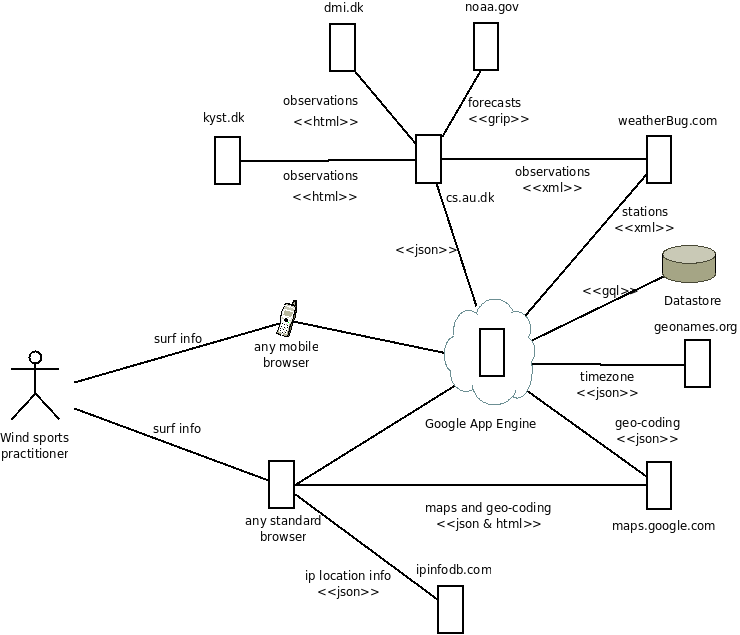
\includegraphics[width=\textwidth]{./Figures/arch_overview}
  \caption{Architectural Overview}
  \label{fig:tech_diagram}
\end{figure}

\section{The Problem}
This section gives an overview of the problem and the problem domain by
presenting the potential users of the system and the task they currently
perform. Finally, we present three scenarios which are visions of how the mashup
will assist practitioners of wind sports

\subsubsection{Users}\label{sec:user_and_task}
Wind- and kitesurfers are users of the application. Little statistic data exist
about this segment of the population. However, a 1994 survey \citep[p.27]{survey:windsurfers}
shows that there are in the proximity of one million windsurfers in the US, where
59.6 per cent are male, and 56.6 per cent of the windsurfers are in the age
interval 25 - 44. An article from
2004 speculates that windsurfing is a growing sport with over 20 million windsurfers
worldwide mostly between 15 and 40 years of age.\footnote{\url{http://www.westcountrynow.com/main/articles/display.cfm?r=0.15720977&ref=417}}

\subsubsection{Tasks}
When wind- and kitesurfers are on call for surfing they continuously check
available weather data for favorable weather conditions. Favorable conditions
mean suitable wind speed in a suitable direction. The suitable direction is
defined by the location of the surf spot (a suitable place for wind- and
kitesurfing). It is dangerous to surf in offshore wind conditions, unless the
surfer is accompanied by a boat to fetch the surfer drifting to the sea. Suitable
wind speed is about 6m/s and above. The users rely on two types of weather data:
forecasts and observations. The two types of data are located at different
sources. \\\\ \textit{Forecasts:} The currently most detailed source for wind
forecasts in Denmark is the wind service of the Danish Maritime Safety
Administration\footnote{\url{http://ifm.frv.dk/index.asp?USER=SURFERE}}
(DMSA). The page, shown in Figure~\ref{fig:frv}, contains a map with a wind
forecast for the current hour in the form of arrows and colors that indicate wind
velocity. The page provides options to access forecasts for the following hours
up to 48 hours in the future from the time of forecast calculation. The
calculations are started every six hours.

\begin{figure}[htbp]
  \centering
  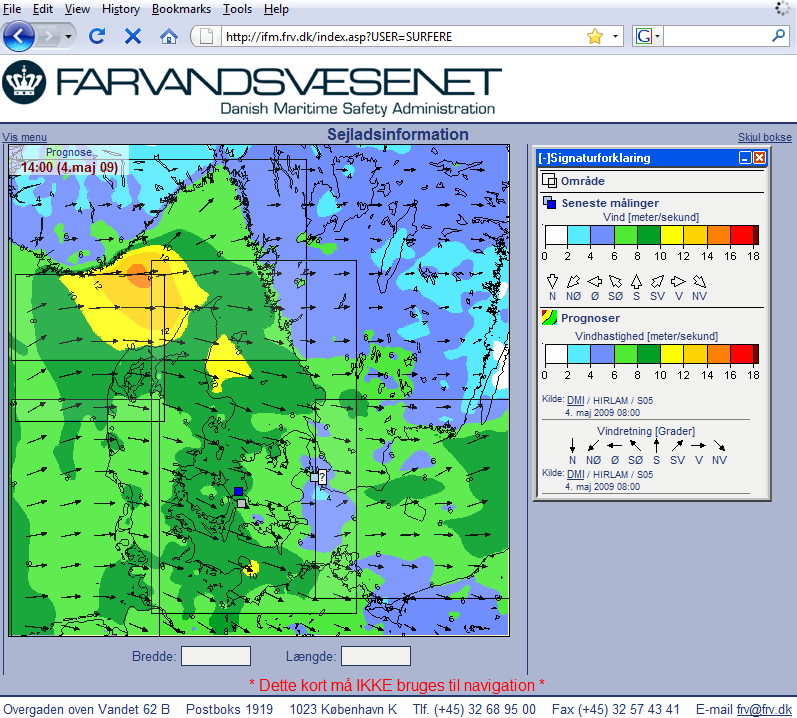
\includegraphics[width=\textwidth]{./Figures/frv}
  \caption{DMSA wind forecast page}
  \label{fig:frv}
\end{figure}

The task users execute with DMSA's service is mapping between the colors and
arrows on the page, and relevant surf spots known to the surfer. Surfers execute
that task at least one time every day when they want to surf.  \\\\
\textit{Observations:} Sources for current wind conditions are the Danish Coastal
Authority\footnote{\url{http://www.kyst.dk}} (DCA), the Danish Meteorological
Institute\footnote{\url{http://www.dmi.dk}} (DMI), and
WeatherBug\footnote{\url{http://www.weatherbug.com/}} (WB).

The service at
DMI\footnote{\url{http://www.dmi.dk/dmi/index/danmark/borgervejr.htm?param=wind&map=undefined}}
shows a map with some of the weather stations and their current
measurements. Detailed information about a weather station is accessed from a
standard browser by clicking on it. The detailed information includes a graph of
the wind measurements for the last 24 hours. Users map between the conditions at
weather stations and spots to check if the current conditions allow for
surfing. This can include an investigation of the graph to see whether the wind
is picking up or slacking down.

\subsubsection{Scenarios}\label{sec:scenarios}
We now present real world scenarios illustrating the benefit of using the
We Love Wind mashup (scenarios are small stories that tell what people do with the
Web site and not how they do it).

\begin{scenario}\label{scenario:one}
  Jacob has just got off work. He wants to know if he can surf in the proximity.

  Jacob accesses the We Love Wind site from his mobile. The site shows that
  currently and the next 4 hours it is possible to surf at a surf spot near Aarhus, he
  decides to go.

  Before rigging his kite Jacob accesses the page again and checks the current
  observations to get a feeling of what size of kite he should use.
\end{scenario}

\begin{scenario}\label{scenario:two}
  One morning, Jens wants to know whether the day is going to be a surf day. He
  accesses the We Love Wind site from any device (mobile device or standard
  computer). The page tracks his location and the page shows tailored spot
  forecasts for the area. He looks at the forecasts and decides to plan for
  surfing in the afternoon.
\end{scenario}

\begin{scenario}
  Brian is on holiday in Skagen. He accesses the We Love Wind site to check
  out the forecasts and the current observations for surf spots near Skagen. The
  site does not have a surf spot for his location.

  In order to get observations and forecasts for the surf spot he decides to
  input a new spot into the site. Afterwards, the site shows observations around the
  spot and wind forecasts for the surf spot.
\end{scenario}

\section{Related Work}
Working with mashups is a cross-disciplinary area. Mashup construction includes
concepts and technologies from a wide and diverse area. This includes Web
technologies and geographic information systems. The following sections present
the important related work in those categories. In addition, we present another
mashup similar in concept to the We Love Wind mashup.
 
\subsection{Geographic Information Systems}
Geographical information systems are systems that associate geographical points
with information.

An important aspect of these systems is serving geographic data
effectively. Geographic data are multi-dimensional -- it typically has a latitude
and a longitude and maybe an altitude -- and therefore usual one-dimensional
database indices are inappropriate \citep[p.173]{multidimensionalaccess:Gaede97}.

A space-filling curve is a curve that parses through each point in a square (it
can be generalized to any dimension). Space-filling curves map values from a
multi-dimensional space to a one-dimensional value. Space-filling curves
therefore support one-dimensional indexing methods. Examples of space-filling
curves for multi-dimensional indexing are the Hilbert space-filling curve, and
the z-order \citep[p.199]{multidimensionalaccess:Gaede97}.

Figure~\ref{fig:z_order} shows a z-order space-filling curve. Cells in the grid
are recursively assigned a one-dimensional value, called the z-value, that
indicate its location in space. The z-value is calculated by cyclically taking
one bit from each coordinate (in the figure, x and y respectively) of the cell and
appending that bit to the z-value \citep[sec.9]{sfc:lawder}. Thus, the
coordinates are interleaved in the z-value. Decoding a z-value to a point in two
dimensions goes as follows: given a z-value such as $11111_2$ (in the figure the
cell most South-East), the space is recursively divided in two starting from the left in
the bit string; even bits pertain to the y-axis, odd bits pertain to the x-axis.

The values of a space-filling curve have the property that the proximity of points
in space is preserved to some extent
\citep[p.199]{multidimensionalaccess:Gaede97}, and that usual database indices,
such as B-trees \citep{btree:bayer72}, can index the values of the space-filling
curve since they are total ordered.

\begin{figure}[htbp]
  \centering
  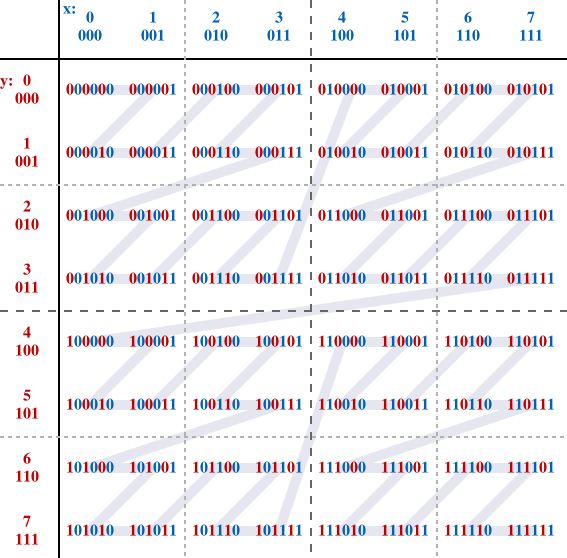
\includegraphics[width=10cm]{./Figures/z-order}
  \caption{Z-values for two dimensional z-order curve \citep{wiki:z_order}}
  \label{fig:z_order}
\end{figure}

Geohash is an algorithm to convert between latitude and longitude coordinates and
a hash value. The term geohash is un-described in the literature the only source
being a Wikipedia article \citep{wiki:geohash}. Geohash values have the essential
property that points in the proximity of each other often have similar geohash
prefixes; therefore, a database can benefit from a string index on the geohash
value of points when performing searches for points in the proximity of each
other.

Geohash is reminiscent to z-order space-filling curves. Geohash divides space in
32 squares recursively; z-order divides space in 4 squares recursively. The
interleaving of two-dimensional points in z-values is the same scheme applied
in geohash.

Geohash is used in \citep{geohash:neighbors}; this implementation includes an
algorithm that returns adjacent locations in the grid. The approach is
un-documented, the implementation being the only
reference.\footnote{Unfortunately, the available example uses JavaScript
functions that are not widely supported. The code uses
\verb+Array.prototype.indexOf+ which is not defined in the ECMAScript Language
Specification. As a result many browsers are unable to execute the
page. The author has, however, successfully opened the page in Google Chrome and
Opera 9.}

\citep{linearquadtree:gargantini} presents a technique to find adjacent location
in grids that takes time for the worst case proportional to the length of the
encoded string. \citep{constantlqtree:aizawa} have improved the algorithm to find
adjacent neighbors in $O(1)$, constant time, in the worst case. The techniques
were immediately applicable for geohash if the number of squares -- i.e., chars
in the base string -- in geohash were a power of four.

\subsection{Web Technologies}
Mashups rely on Web technologies which is an ever evolving area. In this
dissertation we use a subset of Web technologies: Hypertext Transfer Protocol
(HTTP), Hypertext Mark-up Language (HTML), ECMAscript (JavaScript), JavaScript
Object Notation (JSON), and Google App Engine (GAE) to name a few. We introduce
the technologies on the go in the dissertation.

%%  \citep{w3:HTTP} as the application-level
%% protocol. HTTP is a request/response protocol used to interact with resources and
%% parse representations of resources around in a distributed system. We use HTTP to
%% send representations in HTML, ECMAScript (JavaScript from now except when
%% explicitly referring to ECMAscript), and JSON format
%% \citep{w3:HTML,ECMA,json:fat-free}.

%% This includes Web technologies, such as XML, JSON, HTML, HTTP, URI, AJAX,
%% JavaScript, Web scraping, Web Services and hosting.

%% \url{http://aws.amazon.com/ec2/} Amazone EC2 the programmer has direct control
%% with the machine. Responsible for the infrastructure, whereas in the Google App
%% Engine the whole infrastructure is locked. This means the programmer has responsible for
%% everything including scaling which is handled automatically on the Google App
%% Engine.

%% \url{http://www.sun.com/solutions/cloudcomputing/index.jsp}
%% \url{http://www.aptana.com/cloud}
%% infrastructure as a service
%% platform as a service
%% \url{http://www.davidchappell.com/CloudPlatforms--Chappell.pdf}

%%\subsection{Mashups}            
%% Yahoo Pipes
%% Weather Forecasts
%http://developer.yahoo.com/geo/geoplanet/
%%%%% http://www.geonames.org/export/JSON-webservices.html

\subsection{A Similar Web Application}
\url{windguru.com} is a weather service specialized for wind sports. The site
uses global weather forecast data, and finer detailed data for North America, and
Europe. \url{windguru.com} is interesting since it is very detailed and enable
users to setup customized pages with forecasts of their own choice in terms of
location and forecast model.


\part{The Foundations}

\chapter{Web Services}\label{chap:web}
In this chapter we lay out foundations for the architecture of Web Services. We
introduce the Resource Oriented Architecture (ROA): a concrete architecture for
Web Service that is constrained by REST. REST builds on the concepts of software
architecture and architectural style; in order to define and understand ROA and
REST it is necessary to define these two concepts first. We introduce the
necessary terminology for Web Services, Software Architecture, REST, and
ROA. Finally, we give a short intro to HTTP caching.

\section{Web Services}
\begin{definition}\label{def:ws}
A Web Service is a software system that support machine-to-machine interaction
over a network via HTTP.
\end{definition}
The definition is a relaxed version, removing the requirements to use
\textit{\gls{gls:wsdl}} and \textit{\gls{gls:soap}}, of the W3C definition
\citep{w3:ws-glos}. In addition, \textit{support} is interchanged with
\textit{designed for} making any Web site accessible by computers also
fall into the category of Web Services.

The Web Services specifically designed for machine-to-machine interaction
typically fall into one of the two categories: RESTful Web Services and Web
Services based on \gls{gls:wsdl}, \gls{gls:soap}, and the \textit{\gls{gls:ws}}
-- known as \textit{\gls{gls:bigws}}. Creating just the smallest Web Service with
Big Web Services demands an excessive amount of plumbing. In a Big Web Service
implementation several things must be defined: the message formats (in SOAP),
data type definition (in XML Schema), and an interface definition (in WSDL). The
plumbing is due to creating a tight contract forcing everything into a standard.

There, however, already exist a standard that has the plumbing in place, Web
Services based on REST with HTTP and Uniform Resource Identifiers (URI). Web
Services based on REST have the great advantage that the means to work with them
are simple. On the client side, the Web Services are accessed with existing
browsers; on the server side, the Web Services are implemented with usual
technologies to create dynamic Web sites. There are scenarios where a RESTful
approach probably wont do the job, such as a distributed transaction protocol
\citep{infoq:rest_ts}. A Web Service under the constraints of REST, however, is
the approach with the lowest entry barrier, and the approach that work with and
not against the nature of the Web, therefore, we decide to travel light, with
REST.

\section{Software architecture and style}
\begin{definition}\label{def:sa}
  A software architecture is the structure(s) ``of a computing system, which
  comprise software elements, the externally visible properties of those
  elements, and the relationships among them'' \citep[p.21]{sa:bass-ch2}.
\end{definition}

The \textit{\gls{gls:defacto}} definition of software architecture,
Definition~\ref{def:sa}, tells that software architecture is first and foremost
an abstraction of the system. The focus is not on internal properties, but on
visible aspects of the system and how the components in the system cooperate.

An important thing about the software architecture is that it is a basis for
archiving quality in the system it pertains to. A software architecture always
facilitates and prohibits different \textit{\gls{gls:qa}}. Ensuring certain
\gls{gls:qa} in the system is done by constraining the architecture in ways known
to affect these; usually facilitated by the use of architectural styles. We
define an architectural style, based on the definition in
\citep[p.24]{sa:bass-ch2}, as follows:
%
\begin{definition}
  An architectural style is a general solution to a problem that describes
  element and relation types and constraints on their use in the software
  architecture.
\end{definition}
%
\textit{The} most important aspect of architectural styles (styles from now) are
that an architecture that satisfy a style exhibit well known \gls{gls:qa} imposed
by the style \citep[p.~25]{sa:bass-ch2}.

\section{REST}
REST is a style designed for systems that handle \textit{\gls{gls:disthyp}}
\citep{rest:Fielding02}. REST defines a set of architectural elements and
constraints on the use of them that facilitate \gls{gls:qa} relevant in a
context of \gls{gls:disthyp}.

REST is the sum of applying several styles for network-based architectures;
Table~\vref{tab:REST} summarizes the styles; the summary includes a short
description of the styles and their effect on a system in terms
of \useGlosentry{gls:qa}{quality attributes}.

The most characteristic style for REST is uniform interface. It defines several
architectural elements and constraints on the use of them. A pivotal
architectural element of the uniform interface is the resource. 

\begin{definition}
A resource is any information that can be named \citep[p.125]{rest:Fielding02}.
\end{definition}
Resources are uniquely identified by a resource identifier. In terms of the Web,
a resource is any information identified by a \textit{\gls{gls:uri}}. Clients that request a
resource get a representation of the resource -- not the resource itself -- in a
format depending on the capabilities of the client. Interaction with resources
are performed through their representations by passing the representations around
in messages and applying the uniform interface on them. Messages are
self-descriptive, which decouples them from the underlying transport layer;
enabling intermediate servers to cache messages, forward messages, etc.

REST stands for Representational State Transfer. The following quote explains the
meaning of it:

\begin{quote}
\footnotesize\itshape
The name ``Representational State Transfer'' is intended to evoke an image of how
a well-designed Web application behaves: a network of Web pages forms a virtual
state machine, allowing a user to progress through the application by selecting a
link or submitting a short data-entry form, with each action resulting in a
transition to the next state of the application by transferring a representation
of that state to the user. \citep[p.116]{rest:Fielding02}
\end{quote}

An architecture that follows the architectural style of REST is called RESTful. A
RESTful architecture exhibits well known \useGlosentry{gls:qa}{quality
attributes} chosen by the designers of REST. Since REST is a model of how the Web
\textit{should} work \citep[p.116]{rest:Fielding02}, a RESTful architecture will
facilitate \useGlosentry{gls:qa}{quality attributes} deemed relevant for the Web.

\section{ROA: A RESTful architecture}
A concrete RESTful architecture is the Resource-Oriented Architecture
\citep[ch.4]{rest:webservice}. ROA is designed specifically for Web
applications; ROA therefore shows how REST is applied using the intrinsic
technologies of the Web, such as HTTP and \gls{gls:uri}. ROA hereby turns
the constraints of REST concrete. By using HTTP many of the styles from
REST are already satisfied:
%%
\begin{itemize}
  \item Client-server: in HTTP only the client is able to make
  requests, while the server is ready to receive them.
  \item Cache: HTTP provides several caching mechanisms, presented in
  Section \ref{sec:caching}.
  \item Code on demand: via HTTP it is possible to transfer
  programs, e.g., JavaScripts or Java applets, to the client and execute them
  locally.
  \item Layered system: HTTP is the medium for client-server
  interaction; what technology, platform,  etc., the server is based on is hidden
  for the client.
\end{itemize}
%%
That many of the styles of REST are already satisfied comes as no surprise: REST
is the style for HTTP and \gls{gls:uri}. ROA ignores the styles a Web application
cannot affect and instead focus on only four styles; each is described in the
following sections.

Throughout this section we examine an existing Web application to give examples
of violations of the styles and their consequences.  The examples
illustrate some of the advantages of a RESTful Web Service by examining the
inverses. The inverses are so common that we denote them as
\textit{\gls{gls:anti_patterns}}. The Web service examined is
\url{rejseplanen.dk}; a journey planning Web Application for bus and train trips in
Denmark.\footnote{\url{rejseplanen.dk} uses HAFAS planning software which is in
use in 16 countries \url{http://www.hacon.de/hafas/}}.

\subsection{Addressability}
Since ROA is based on REST it is centered around the resource architectural
element. In ROA all interesting information provided by the server is a
resource. Resources are identified by a \gls{gls:uri} with a reasonable name
reflecting the concept of the resource \citep[Ch.4]{rest:webservice}. Data on the
server not exposed by a \gls{gls:uri}, are not resources. This
constraint, known in ROA as addressability, gives several advantages:
%%
\begin{itemize}
  \item The provider of data is separated from the consumer of data which
  decouples the application. The decoupling introduces support for arbitrary
  composition of the resources at the client side -- known as mashups.
  \item Caching mechanisms in HTTP have a larger basis to work
  on, because they have a larger contact area with the Web application.
  \item Clients can link to and bookmark specific pages in the Web application.
\end{itemize}
%%
\subsection*{Addressability anti-pattern}
Some Web applications do not expose their interesting information through
\useGlosentry{gls:uri}{URIs}. An example of a web application that violates
addressability is \url{rejseplanen.dk}.

Journey plans from \url{rejseplanen.dk} is shown in
Figure~\ref{fig:rejseplanen_addr}. We arrived at the page after filling out a
search form on the front page, entering the information that we want to go from
Aarhus to Copenhagen, and submitting the form.

%% Behind the scenes, the form submits its values with the
%% \verb|POST| method to \url{http://www.rejseplanen.dk/bin/query.exe/en}.

In the figure we notice that the \gls{gls:uri} of the journey plan page is
unchanged when compared to the main page. This makes it impossible to link to the
journey plan, since the \gls{gls:uri} in the address bar does not reflect the
page currently visited; therefore it is not addressable. The only address ever
exposed in the address bar is the \gls{gls:uri} of the main page. The reason is
that the page uses frames. From a usability perspective, the use of frames was
discouraged already in 1996, because it destroyed addressability
\citep{nielsen:frames}. The addressability violation has a severe impact on the
application: bookmarking the journey plans page is disabled, and the provider and
consumer of data are coupled.

What if the frames are removed? The site expose a search resource, namely the
search engine interface, and not the interesting data behind it. This is contrary
to similar search services, e.g., Google that exposes their data. A Google URI
like \url{http://www.google.com/search?q=addressability} returns a representation
of the directory of the 10 most relevant pages containing the term
addressability. 

%% Creating an addressable Web application, \url{rejseplanen.dk}
%% could expose journey plans resources such as
%% \verb|www.rejseplanen.dk/search?q=aarhus,k�benhavn/|.

%In fact \url{rejseplanen.dk} at their site states wants their web service used by
%both humans and computers \footnote{http://info.rejseplanen.dk/index.php?pageid=208}

%rejseplanen.dk/search?q=aarhus+''my+road'',k�benhav/n

\begin{figure}[htbp]
  \centering
  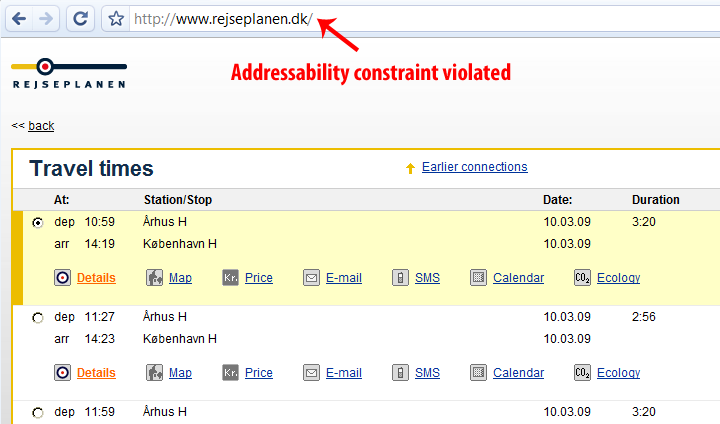
\includegraphics[width=\textwidth]{./Figures/rejseplanen_addr}
  \caption{Addressability violation; [accessed 11-March-2009]} 
  \label{fig:rejseplanen_addr}
\end{figure}

\subsection{Statelessness}
\label{sec:statelessness}
The style of statelessness is enforced in ROA by using HTTP. By design HTTP is
stateless; a workaround is needed to introduce state. An example of this is
cookies \citep[p.145]{rest:Fielding02}. Cookies usually contain a hashed value
referring to a data structure on the server containing
\textit{\gls{gls:appstate}}. Since \gls{gls:appstate} is saved on the server the
stateless style is violated. Cookies used in this way circumvent the quality
advantages introduced by statelessness since servers must use resources to store
client state and replicate state across servers in a clustered environment.
%% http://msdn.microsoft.com/en-us/library/ms525473.aspx

\subsection*{Statelessness anti-pattern}
Many Web applications use cookies to support session state, e.g.,
\url{rejseplanen.dk}. Storing application state for each user demands an
excessive amount of resources on the server. Resources are regained by garbage
collecting session data structures after a short amount of idle time -- typically
less than 20 minutes. Re-accessing a site after the 20 minutes idle time causes
an error because the data structure is removed;
Figure~\ref{fig:rejseplanen_state} shows what happens when we re-access the
journey plans: it causes a failure degrading usability.

In the previous section we criticized the page for violating addressability, but
now it makes sense that the page is not addressable. The statelessness violation
totally removes the option to make the application addressable since all pages
are invalidated after a short amount of time.

\begin{figure}[htbp]
  \centering
  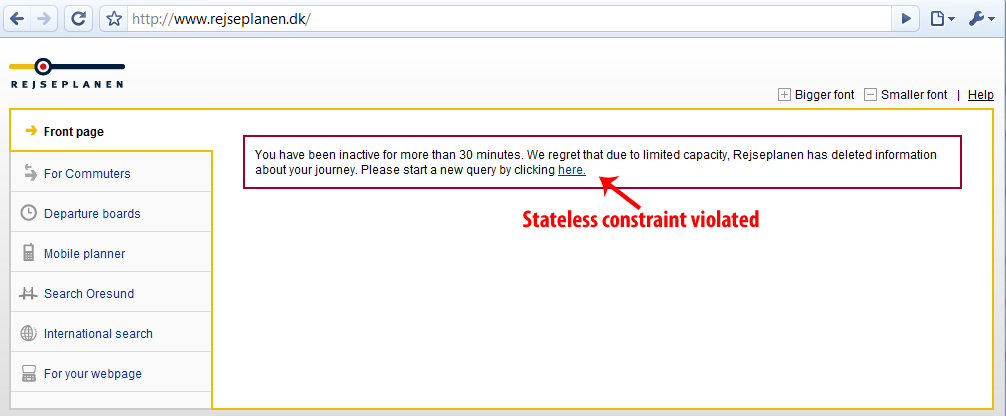
\includegraphics[width=\textwidth]{./Figures/rejseplanen_state}
  \caption{Stateless violation; [re-accessed 11-March-2009]}
  \label{fig:rejseplanen_state}
\end{figure}

\subsection{Uniform interface}\label{sec:ws_uniform_interface}
Clients of RESTful Web Services interact with a resource, through HTTP and the
\gls{gls:uri} of the resource. ROA demands the proper application of the HTTP
methods \citep[ch.4]{rest:webservice}. HTTP defines eight methods that can be
performed on a resource each with well defined semantics \citep{w3:HTTP}. The
semantics of the important methods are given in Table~\ref{tab:HTTP}; it is
indicated whether the methods are idempotent and whether they are safe. Safe and
idempotence are terms defined in \citep{w3:HTTP}. Safe denotes the property that
a method is free of side effects that the user can ``be held accountable
for''. Idempotence denotes the property that ``the side-effects of $N > 0$
identical requests is the same as for a single request.'' The definition of
idempotence is unclear unless side effects are interpreted as the side effects the
user can be held responsible for, e.g., GET is an idempotent operation but in
many cases a GET request changes the server state by writing to the server log,
causing some caching, incrementing a page counter etc. Interpreting side effects
as user responsible side effects allow side effects, such as incrementing a
counter and writing to the log, and does not violate the property of idempotence;
in addition the safe methods become a proper subset of the idempotent methods.

There exist a problem in supporting the uniform interface of HTTP on the
Web. (X)HTML forms only support two HTTP methods: \verb|GET| and \verb|POST|
\citep[sec.17]{w3:HTML}. A workaround is to overload the \verb|POST| method, by adding,
e.g., a \verb|_method| parameter to the query parameters, and route to the
corresponding implementation on the server. To \verb|PUT| or \verb|DELETE| a
resource from a Web browser a form then needs to \verb|POST| to the following
URIs respectively:
%
\begin{verbatim}
  {resource_uri}/?_method=PUT
  {resource_uri}/?_method=DELETE
\end{verbatim}
%

\begin{table}[htbp]
\centering
\setlength\extrarowheight{3pt}
\begin{tabularx}{\textwidth}{l X}
\toprule
HTTP Method    & Semantics\\\midrule
\verb|GET|
               & Retrieve the representation of a resource pointed to by the URI (safe).\\
\verb|HEAD|
               & Same as GET except the response only consist of header fields (safe).\\
\verb|PUT|
               & Create or update the resource identified by the URI in the HTTP message, 
with the representation of the resource located in the body of the HTTP message (idempotent).\\
\verb|DELETE|
               & Delete the resource identified by the URI in the HTTP message (idempotent).\\
\verb|POST|
               & Post the data located in the body of the HTTP message as a new subordinate of %
the resource identified by the URI in the HTTP message (un-idempotent).\\
\bottomrule
\end{tabularx}
\caption{HTTP Methods and their semantics \citep[sec.9]{w3:HTTP}}\label{tab:HTTP}
\end{table}


\subsection*{Uniform interface anti-pattern}
The query interface of \url{rejseplanen.dk}, which consists in an HTML
form, is an example of an illegal use of the HTTP methods in terms of
their semantics. The form uses \verb|POST| to send the query, however, it makes
no sense for the server to create a subordinate resource, in reaction to the
request. 

Browsers notice the use of \verb|POST| and some, e.g., Google Chrome and Safari,
ask for a confirmation when using back / forward buttons, ruining the user
experience, as shown in Figure~\ref{fig:rejseplanen_form}. The warning is
perfectly valid if \verb|POST| is used correctly, namely for posting some data at
the server. In this case, however, it is a misuse of the method; the method is
safe doing nothing besides retrieving data and therefore \verb|GET| should be
used. 

Another unfortunate side effect of the misused \verb|POST| method is that, by
definition, clients must invalidate their cached representation when POST is used
\citep[sec. 13.10]{w3:HTTP}, taking away the advantage of caching.
  
\begin{figure}[htbp]
  \centering
  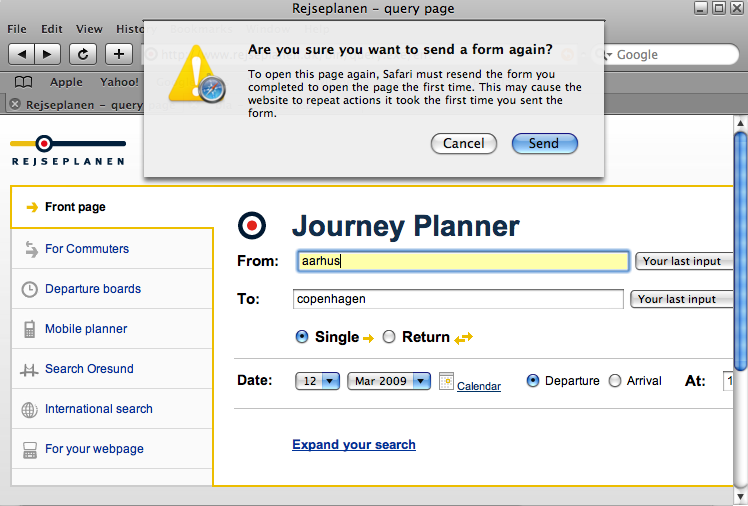
\includegraphics[width=\textwidth]{./Figures/rejseplanen_form_resubmission}
  \caption{Warning message in Safari because of uniform interface violation; [accessed 12-march-2009]}
  \label{fig:rejseplanen_form}
\end{figure}
There are two probable explanations for the illegal use:
%%
\begin{enumerate}
  \item Web crawlers refrain from taking the search link because it uses
    \verb|POST|; reducing use of resources on the server. \url{rejseplanen.dk},
    however, has disabled indexing of all their site, see
    Appendix~\ref{app:fig:rejseplanen_robots}; therefore, resource consumption by
    friendly bots are not a problem.

  \item Internet Explorer imposes a maximum length on URIs to 2,083
    characters\footnote{\url{http://support.microsoft.com/default.aspx?scid=KB;en-us;q208427}}
    although no limit exists in the HTTP specification \citep{w3:HTTP}. The
    limitation does not exist for \verb|POST|, since values in a \verb|POST|
    message does not go into the URI.

    The length of the encoded form is 1562 characters, This is without the
    from-city, the to-city, and a optional via-city. Thus there are over 500
    characters left to encode only 3 places, surely enough, also rendering this
    explanation invalid.
\end{enumerate}
%%
Both reasons are invalid reasons for using \verb|POST|. The explanation probably
lies in \url{rejseplanen.dk} ignoring the HTTP specification, causing unfortunate
side effects for the Web application.

%% http://www.w3.org/Provider/Style/
%% http://www.w3.org/2001/tag/doc/whenToUseGet.html


\subsection{Connectedness}
The style of connectedness states that resources in a Web Service should be
linked together.

\subsection*{Connectedness anti-pattern}
The human Web is a myriad of connected pages in contrast to many Web Services. In
Web Services, connectedness is often forgotten \citep[p.~96]{rest:webservice};
disallowing users ``to progress through the application by selecting a link or
submitting a short data-entry form'' breaking REST. The problem is easily
illustrated by an example: contrast the JSON representation of weather stations in
Listing~\ref{lst:connected_weather_stations} with the representation in
Listing~\ref{lst:ill_weather_stations}.

\begin{lstlisting}[caption=Connected weather stations representation, label=lst:connected_weather_stations]
{
  "next": "/api/weather_stations/?geohash_offset=swgv3sxf003p"}  
  "items": [
    {
      "name": "Skagen", 
      "lat": 57.723952722299998, 
      "lon": 10.5997467041016, 
      "timezone": "Europe/Copenhagen", 
      "type": "DCAWeatherStation", 
      "uri": "/api/weather_stations/dk/skagen/",
      "uri_extern": "http://www.kyst.dk/sw3029.asp", 
      "uri_observations": "/api/weather_stations/dk/skagen/observations/", 
      "uri_scrape": "http://www.kyst.dk/custom_asp/defaultjs.asp?id=3003&targetStation=1100"
    },(...)
  ]
}
\end{lstlisting}

The former is a connected resource containing links to other resources. The
latter is disconnected. A client of the disconnected Web Service must know all
the relevant \gls{gls:uri}s. Clients are bound to break if the Web Service
changes its \gls{gls:uri}s. A Web Service violating connectedness results in a
close coupling between the client and the server.

In a RESTful, i.e., connected Web Service links between resources are available
in the representations, such as \verb|uri_scrape| and \verb|observations| in the
connected example. The added level of indirection decouples clients from the
server since they are now able to use references, instead of direct links, to
resources.

\begin{lstlisting}[caption=Unconnected weather stations representation, label=lst:ill_weather_stations]
{
  "page": 1,
  "has_next": true,
  "items": [
    {
      "name": "Skagen",
      "lat": 57.7239527223,
      "lng": 10.5997467041,
      "type": "DCAWeatherStation", 
      "timezone": "Europe/Copenhagen"
    }
(...)]}
\end{lstlisting}

\section{Caching}\label{sec:caching}
Caching is about one overall thing: reducing the amount of traffic to transfer
over the network. Caching is not a requirement in ROA; however, caching is
pivotal in reducing the latency of Web Services. This section presents the
foundations of HTTP caching.

HTTP caching is a set of mechanisms defined in \citep[Sec. 13]{w3:HTTP} that
indicate to clients and servers which resource representations are cacheable
and when they are stale.

HTTP caching is applied by setting appropriate HTTP headers in the
responses from the server. Advanced clients, such as browsers, perform
caching based on these headers. The content in the caching headers can
be seen as validators; additional client requests trigger the
validators. Only if the validatores are true the client should update
its resource representation.

The caching style of REST (i.e., responses are ``implicitly or explicitly labeled
as cacheable or noncacheable'' \citep[p.121]{rest:Fielding02}) is satisfied in any
HTTP application: if no caching directives is set responses may be cached,
however, it is not expected \citep[sec.13.4]{w3:HTTP}.

There exist three headers to cease explicit control over HTTP
caching:\footnote{We ignore the older caching headers from HTTP 1.0: Expires and
Last-Modified.} \verb|Cache-Control|, \verb|ETag|, and \verb|Vary|; each are
described in the following.

\subsubsection*{Cache-Control}
\verb|Cache-Control| is a header field that controls the valid duration of cached
responses. The field can specify that a cached resource is valid for a relative
time duration. In that time duration all contact with the origin server on
additional requests for the same resource is bypassed.

A header response that defines that the \textit{\gls{gls:ttl}} of a cached
representation is 3600 seconds and applies for all clients, looks like
the following:

\begin{verbatim}
Cache-Control: public, max-age=3600  
\end{verbatim}

A response can also be marked as non-cacheable. The \verb|Cache-Control| field is
the concrete means to do the marking by setting value to \verb|no-cache|. There
is a subtlety in \verb|no-cache|: clients are still allowed to cache responses,
however, before applying the cache they must contact the server to validate that
the cached version corresponds to the server's version. Validation puts forth a
requirement of identifying different versions of a resource, manifested in the
\verb|ETag| field.

\subsubsection*{ETag}
When \gls{gls:ttl} of a representation is overdue the client might still use the
cached version.

\verb|ETag| is a unique identifier attached to resources in requests and
responses. With \verb|ETag| servers validate whether clients' local cached
representation is stale by comparing the \verb|ETag| of the local representation
against the \verb|ETag| of the resource at the server. The server only sends back
a representation upon mismatch of the \verb|ETag|s.

\textit{Note:} Uniqueness of \verb|ETag|s are only in terms of identifiers under
the same URI; therefore, e.g., the last time of modification is a valid \verb|ETag|
value, assuming that no two updates of the same resource can be processed in the
same time frame.

The gain of using \verb|ETag|s is a reduction of the amount of data which are
sent over the network; the total number of requests and responses remain unchanged.

\subsubsection*{Vary}
Since \verb|ETag|s are used to compare a client's representation of a resource
against the \verb|ETag| of the resource at the server, the cache might serve the wrong
representation, but with the correct \verb|ETag|. A common example: given a Web
Service that does \textit{\gls{gls:content_negotiation}} on the type of user
agent, e.g, a mobile user agent or a desktop user agent, a cached response must
only be served to clients of the same type. The \verb|Vary| header field comes to
the rescue and indicates to the client the header fields that can vary the
representations of the resource. The following line indicates how this is
indicated in the HTTP header:

\begin{verbatim}
Vary: User-Agent
\end{verbatim}

\section{Summary}
In this chapter, after having introduced the terms of REST and ROA, we showed
what advantages a RESTful Web Service provides. The advantages were illustrated
by giving examples of a Web Service that violates the styles of REST, and by
discussing the disadvantages the REST violations cause. Finally, we looked at
HTTP caching which is important for increasing the performance of Web Services.

  \begin{sidewaystable}[htbp]
    \centering \setlength\extrarowheight{3pt}
    \begin{tabularx}{\textwidth}{l X X}
    \toprule
Architectural style    & Description        & Effect\\\midrule

Client-server          
               & The system is split up into the provider of a service and the consumer of it.  
               & \textit{Performance} and \textit{modifiability} benefit since separating the concerns makes the server and client simpler and localize changes.\\
Stateless              
               & Client state is disallowed on the server therefore all requests must be standalone.
               & Server \textit{performance} increases, since the server can free resources immediately after requests are processed.\newline
Network \textit{performance} decreases, since messages must be self contained and therefore demands more space.\newline
\textit{Availability} and \textit{modifiability} benefit, since requests can be routed to any server containing the service, 
removing issues of coordination in a clustered environment and losing state on server crashes. \\
Cache                  
               & Results of a request are marked as cacheable or non-cacheable.
               & When caching is applied, \textit{performance} increases due to less network communication and less load on the server. However, the complexity of the application increases, and data staleness also becomes an issue. \\
Uniform interface
               & Components are restricted to a general interface. 
               & \textit{Modifiability} benefit since the overall system architecture is simplified and decoupled. \\
Layered system         
               & The system is split up into hierarchic layers, where layers only use functionality from the layer directly beneath it.
               & \textit{Modifiability} increases, as underlying information is hidden and therefore reduces coupling.\newline
\textit{Performance} decreases since communication must pass through several layers.\\
Code on demand
               & Clients are enabled to download code from the server and execute it locally. 
               & \textit{Performance} increases, since code is executed locally avoiding a round-trip to the server. Load is taken off the server and put on the client. \newline
\textit{Usability} increases since the application reduces latency resulting in a more responsive application.\newline
\textit{Modifiability} benefit since features are easily modified and added to the client \\
    \bottomrule
    \end{tabularx}
  \caption{Architectural Styles of REST (quality attributes are in italics)}\label{tab:REST}
\end{sidewaystable}


\chapter{Web Service clients}\label{chap:ws_clients}
A Web Service client is the consumer of a Web Service. According to
Definition~\ref{def:ws} the consumer can be any HTTP client at the other end of
the line, e.g., an Ajax client. In this chapter, we introduce what is probably
\textit{the} most popular style for Web Service clients: Ajax. Ajax is presented
in the light of REST, leaving important things behind, such as the
\verb|XMLHttpRequest| object. In addition, we introduce JSON; a simple data
format for interchanging data between servers and clients.

%and why JSON is chosen as representation
%format for the surf weather service.

%We discuss the advantages of a \textit{\gls{gls:fat_client}} approach for the
%user interface.
\section{Ajax: the style for modern Web Service clients}\label{sec:ajax}
Ajax is a style for a set of Web technologies that narrow the gap between the
``richness and responsiveness'' of desktop applications and Web applications
\citep{ajax:coined}. Initially, the technologies used in Ajax were incorporated in
the name itself. Ajax is short for Asynchronous JavaScript + XML; however, in
many newer Web applications the XML has been replaced by JSON.

In Ajax applications, an Ajax engine on the client side extends the HTTP
request-response cycle by communicating asynchronously with the
server. Traditionally, in server-side Web applications, a client's request result
in the server crafting and returning a unique HTML page to the user. The Ajax
style, however, allows for putting the logic of crafting the page on the
client\footnote{The Ajax style also allows for small page updates of a site
crafted at the server; this is, however, not the focus of this section.}, and
lets the server handle pure \textit{\gls{gls:business_logic}}. The approach has
the following advantages:
\begin{itemize}
  \item the server is relieved of compositioning Web pages;
  \item the presentation of data at the client is separated from the producer of
  it; and
  \item the Web application can be made more rich and responsive.
\end{itemize}
Most server-side applications that customize pages violate the REST style of
statelessness: \textit{\gls{gls:appstate}} is put on the server in order to
create customized pages effectively. Maybe the biggest advantage of the Ajax
style is that it can circumvent the problem of customization by placing
\gls{gls:appstate} where it belongs in terms of REST, in the client.

The benefits of the Ajax approach over a usual server-side approach are numerous:
\begin{itemize}
  \item it is possible to create dynamic customized sites with a stateless
server;
  \item static files, such as the Ajax client, are cached at the client after the
user's first access to the page, therefore, on additional requests only new
business data is loaded from the server. Compare this to a server-side approach
where a unique page is created for every user.
\item business data is isolated boosting cache hits on intermediate servers for
all clients. In addition, an optimal caching strategy for each type of component
can be applied. Compare this to a server-side strategy where any change in
the site must invalidate the cache.
\end{itemize}
Thus, an Ajax approach supports REST while at the same making customized Web
sites possible. Hereby the Ajax approach inherits one of the main quality
attributes of REST: scalability \citep[p.116]{rest:Fielding02}

The drawbacks of adopting the approach are that 1) the application needs to be
implemented using several languages: one for the server-side Web Service, and
JavaScript for the client-side; 2) clients need to have JavaScript enabled, and
3) JavaScript is the language of implementation making well-known Web application
frameworks -- and all their tools such as debugging tools -- useless for anything
else than creating Web Services.

%The Ajax client can consume data from different types of Web Services, e.g., Big
%Web Service or RESTful Web Services. Using a RESTful Web Service for serving
%data, however, gives all the advantages stated in the REST architectural styles overview
%in Table~\ref{tab:REST} now apply for the application.


\section{JSON}\label{sec:json}
JavaScript Object Notation (JSON) is a data interchange format. JSON is a subset
of JavaScript and described as ``The Fat-Free Alternative to XML''
\citep{json:fat-free} and indeed since its introduction Web developers and Web
Services have adopted JSON as the simpler and cleaner data interchange format
with companies such as Yahoo and Google embracing JSON
\citep{json:yahoo,json:google}. One of the reasons JSON is
widely adopted is due to its simplicity: the syntax can be described with a
context-free grammar in just a few lines:
\begin{verbatim}
  <Literal> ::= <Object> | <Array> | string_literal | numeral | 
                boolean_literal | null 
  <Object>  ::= {} | { string_literal: <Literal>} | 
                { <Object>, <Object>} 
  <Array>   ::= [] | [<Literal>] | [<Literal>, <Literal>]
\end{verbatim}
In addition, JSON is efficiently used within JavaScript, and JSON can circumvent
the same origin policy. A JSON response is de-serialized into JavaScript objects
by using the JavaScript \verb|eval()| function:
\begin{verbatim}
var data = eval('(' + json_response + ')');
\end{verbatim}
The \verb|eval()| function takes a string as parameter and evaluates it as if it
were JavaScript code directly written in the document. Since JSON is a subset of
JavaScript \citep{json:fat-free} JSON can be de-serialized with
\verb|eval|. However, that approach is subject to \textit{\gls{gls:xss}} if the
response contains user generated data. See Appendix~\ref{sec:xss} for an example
of using a raw eval to inject and execute JavaScript code. Instead of using eval
to de-serialize data we use a JSON parser\footnote{http://www.json.org/json2.js}.

\begin{figure}[htbp]
  \centering
  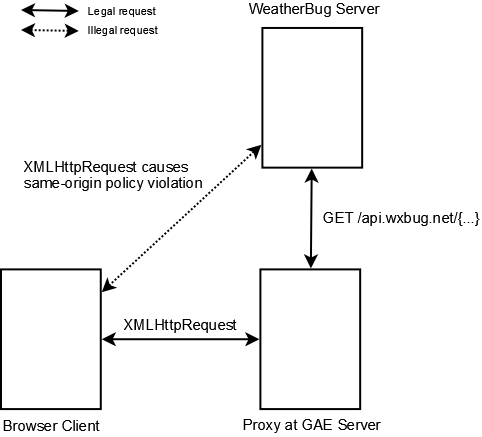
\includegraphics[scale=0.3]{./Figures/proxy}
  \caption{Circumventing the same origin policy with a proxy}
  \label{fig:proxy}
\end{figure}

The same origin policy is a set of security restrictions imposed by
browsers. They prohibit access to methods and properties of documents served from
other origins compared to the document where it is embedded. Origin is defined by
most browsers as the hostname and port number
\citep{browsersec:part2}. Therefore, e.g., external Ajax requests and Document
Object Model (\textit{\gls{gls:dom}}) access to external content in frames are
impossible: the content must stem from the same domain to do this.

A workaround to enable access to cross-domain data is setting up a proxy that
tunnels all request to a server at another domain through the server hosting the
current site. An example where we could have set up a proxy to circumvent the
problem is for XML weather data resources from WeatherBug. The resources are not
in JavaScript format which makes it impossible to load data directly from
WeatherBug into the client. Therefore we could setup a proxy that tunnels all
request to the WeatherBug API through the GAE server, as shown in
Figure~\ref{fig:proxy}.

Another reason for the success of JSON is due to an exception in the same origin
policy: it does not apply for externally valid JavaScript loaded via the HTML
\verb|<script>| tag. Script tags are untouched by the same origin policy, and
therefore many Web Services provide data in JSON format. Client access JSON
Web Service by dynamically creating \verb|<script>| tags and inserting them into
the document; upon insertion the browser fetches the external content into the
document. Now how do we know when that \verb|<script>| tag has finished loading?
If the Web Service is able to wrap the JSON object in a user-chosen function we
have JSONP \citep{json:defined}. With JSONP that user-defined function is called
automatically when the \verb|<script>| tag is loaded. 

\section{Summary}
In this brief chapter we introduced Ajax from a RESTful perspective, which
included an overview of the advantages of the Ajax style where the server is a
pure holder of business data.


% Chapter 1
\begin{savequote}[10pc]
\sffamily 
``The issue is no longer where the information lives - what server, what
application, what database, what data center. It's actually now all about putting
information to work.''
\qauthor{Carly Fiorina (1954-)}
\end{savequote}
\chapter{Google App Engine}\label{chap:gae}
When creating Web applications there is an overhead going from development into
production with the application. The overhead includes setting up several
elements: a Web server, a database, scripts, monitoring, etc. In this chapter, we
introduce and describe the Google App Engine (GAE) which removes the
overhead. We describe the GAE architecture, and based on the description we
present snippets of Web application code and assemble them into a working GAE
application.

\section{What is the Google App Engine?}
GAE is a server and development platform, created by Google. GAE lets programmers
focus on crafting the application and eliminates many server issues. GAE reduces
the time to deploy and automatically scales as the application grows by
providing access to the Google infrastructure. The infrastructure consists of a
serving infrastructure and several Google services, such as
\textit{\gls{gls:googleaccounts}} and the datastore.

The serving infrastructure is encapsulated away from the application
programmer. Behind the scenes, the infrastructure adjusts the resources allocated
to serve the application, depending on the load on it. Outsourcing the serving
infrastructure to Google has the advantage that issues about serving the
application are moved to experts at Google. Server issues include things such as
setting up the server, securing it, making it scale, etc.

Before the programmer can focus entirely on creating the application, there are
still issues regarding both bringing the application online and debugging the
application. Google has put an effort into solving these issues by creating a
local development environment and scripts to bring the application online
instantly.

The advantages come at a cost; a GAE application is limited in numerous ways
\citep{Google:quota, Google:cgi}. In February 2009, the limitations were quite
severe:
\begin{itemize}
  \item only one language was supported, namely Python;
  \item scheduling tasks were impossible, since HTTP requests were the only means
  to start a process; and
  \item long-lasting processing was impossible, since requests could not last longer
  than 10 seconds.
\end{itemize}
Google App Engine is an emerging technology; since the first writing, five months
ago, the GAE is changed in numerous
ways: Google has since added Java support\footnote{\url{http://code.google.com/p/googleappengine/issues/detail?id=1}
}, scheduling of cron jobs\footnote{\url{http://groups.google.com/group/google-appengine/browse_thread/thread/552e9ab4a97abc48?hl=en}
}, however, limited to 20, and increased
the request duration to 30 seconds\footnote{\url{http://code.google.com/p/googleappengine/issues/detail?id=6}
}, and etc..

The limitations are now mitigated, however, essential tasks still \textit{cannot}
be done. The limitations mean that many GAE applications demand workarounds;
thus, when to use GAE is a subjective matter that depends on the type of the
application.

On the other hand, GAE is free and makes it easy to get started with one's
application. Therefore, for a prototype Web application that fit almost within
the limits of GAE, the advantages outweigh the disadvantages, and make GAE
suitable.


%A benefit of GAE, unlike other similar offerings, such as Amazon Elastic Compute
%Cloud\footnote{\url{http://aws.amazon.com/ec2/}} and Aptana
%Cloud\footnote{\url{http://www.aptana.com/cloud}}, is that it is free.
%% Aptana Cloud has no cron job either!!! http://forums.aptana.com/viewtopic.php?f=43&t=5935

\section{An example for the impatient}
Before digging into the GAE architecture we show a 'Hello, world' example for
GAE. The interesting point about the example is how little code is needed to run
the example on the server.

The 'Hello, world' example consists of only two files, given in
Listing~\ref{lst:appYamlHelloWorld} and Listing~\ref{lst:helloWorld}.

\begin{itemize}
  \item \verb|app.yaml|, a configuration file containing handlers. Handlers are a
  list of \textit{\gls{gls:uri}} patterns with descriptions of how requests to \gls{gls:uri}s are handled. In
  this case the server will execute the script \verb|main.py| for all \gls{gls:uri}s. %
  \item \verb|main.py|, a Python \textit{\gls{gls:cgi}} script that output a
string containing a content header and the content, which the server sends back
to the client.
\end{itemize}

\begin{lstlisting}[caption=app.yaml,label=lst:appYamlHelloWorld]
application: helloworld
version: 1
runtime: python
api_version: 1

handlers:
- url: .*
  script: main.py
\end{lstlisting}


\begin{lstlisting}[caption=main.py,label=lst:helloWorld]
print 'Content-Type: text/html'
print                            # end of headers
print '''
<html>
  <head>
    <title>Hello, world</title>
  </head>
  <body>
    <h1>Hello, world</h1>
  </body>
</html>
'''
\end{lstlisting}

The example is run by starting the development server, with the directory of the
two files, as argument. Now accessing \verb|http://localhost:8080| with a
browser outputs \verb|Hello, world|.

\section{Architecture}
\begin{figure}[htbp]
  \centering
  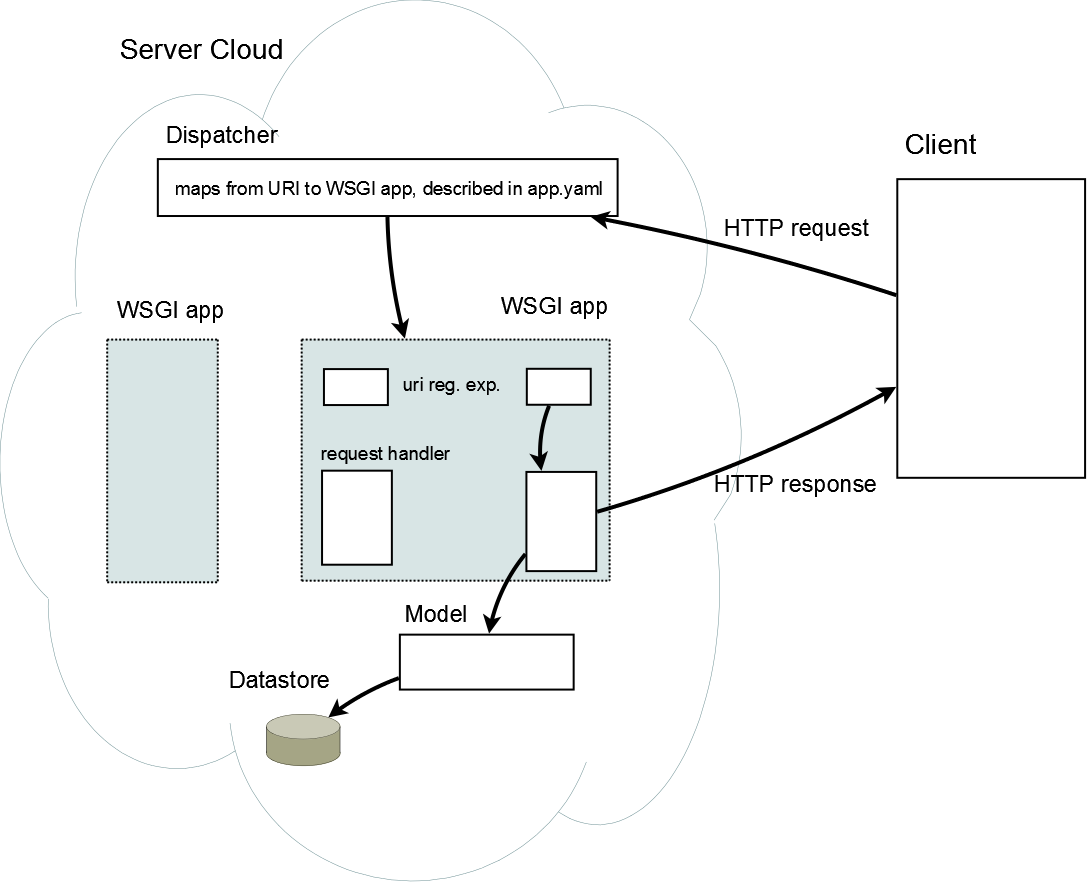
\includegraphics[width=\textwidth]{./Figures/webappArch}
%  \rule{\textwidth}{0.005in}
  \caption{GAE architecture}
  \label{fig:webapp}
\end{figure}
%%The GAE roughly consisting of five things:

%%\begin{enumerate}
%%  \item a serving infrastructure, which connects \gls{gls:uri} requests to a running
%%  instance of the application code somewhere in the %%
%%
%%   \xglossary{name={server cloud}, 
%%              description={ToDo}}%
%%             {\textit{server cloud;}} 
%% %%
%%   \item a Python runtime environment;
%%   \item an SDK which supports development and running of the code locally;
%%   \item administration tools; and
%%   \item the Google database, called datastore.
%% \end{enumerate}

The basic architecture of GAE is illustrated in Figure~\ref{fig:webapp}. Starting
from the client, on the right, incoming \gls{gls:uri} requests are routed to a
corresponding \textit{\gls{gls:wsgi}} application -- the blue squares in the
figure -- somewhere in the server \textit{\gls{gls:cloud}}. Inside the WSGI
applications the requests are routed again to a request handler, which
potentially interacts with the data models, to get relevant data. At last the
server returns a string to the client.

The GAE comes with its own Web application framework called webapp. The Web
server supports any \textit{CGI}-compliant Python application, like webapp or
Django. However, since Django is tied closely together with relational databases,
the Django framework cannot directly be used in GAE. There are different helpers
to work around the database impedance mismatch
\citep{Google:djangohelper,GAE:djangopatch}. For the application in this thesis
we are using the app-engine-patch that adds Django support to GAE.

Crafting Web pages in Django follows the
\textit{\gls{gls:requestresponsepattern}} from HTTP. A Django application
contains request handlers which are Python functions. When a request arrives in
the Django application, it is routed to a request handler and wrapped in a
request object which is given as argument to the handler. Routing is setup
explicitly by regular expression.

Each request handler must return a response object. The handler creates the
response string either explicitly, within the handler, or implicitly with
templates. Templates are used to separate the presentation logic from the request
handlers. Using templates, the architecture can be seen as consisting of three
layers, fitting into the Model-View-Controller style (MVC), shown
in Figure~\ref{fig:mvc}.

The style consists of three architectural components:
\begin{itemize} 
  \item the Model that contains the data and the persistence logic;
  \item the View that takes the data from the controller and produces
a textual response (HTML, JavaScript, etc.); and
  \item the Controller that receives the requests and connects views
and models.
\end{itemize}

\begin{figure}[htbp]
  \centering
  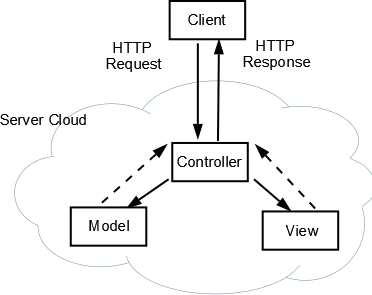
\includegraphics[width=8cm]{./Figures/mvc}
%  \rule{\textwidth}{0.005in}
  \caption{Model-View-Controller architectural pattern }
  \label{fig:mvc}
\end{figure}

The depicted pattern is a variant of the original Model-View-Controller pattern
\citep{RefWorks:28}. Instead of the model pushing updates to the view, the
controller pulls the data from the model, and passes model data to the
view. Therefore there are no connection between the model and the view, like in
the original MVC pattern.

In the following sections, the GAE and Django is described in terms of the MVC
pattern.

\subsection{Model}\label{sec:gae_model}
The models of the application declare the format of, and manipulate the data of
the application. The models are usually stored in a relational database. The
``database'' in GAE is special; it is not a normal relational database,
but a database based on Google's BigTable technology \citep{RefWorks:26}, called
datastore. The best way to think of the datastore is as a database of objects.

GAE comes with an API for datastore interaction, called Datastore API. The API
provides functionality to declare datastore entities, and declare their
properties, directly in Python, based on the \textit{\gls{gls:activerecord}}
pattern. Creating a data model with the Datastore API is easy. The datastore data
models are created reflectively, on their first import, by the GAE from Python
classes that inherits from the \verb|db.Model| class. This means a data model is
a Python class. The content of the data model is declared by defining class
attributes of the type \verb|Property| in the model class. An example model that
represents a surf spot is given in Listing~\ref{lst:spotModel}.

\lstset{language=Python}
\begin{lstlisting}[caption=Spot model,label=lst:spotModel]
from google.appengine.ext import db

class Spot(db.Model):
    name = db.StringProperty(required=True)
    point = db.GeoPtProperty(required=True)
\end{lstlisting}

The spot model uses the built-in property-classes to declare the properties of
the spot data model. The point property uses a richer semantic type
\verb|GeoPtProperty| used to store geographical points consisting of a latitude
and longitude. The API includes many such richer types, such as \verb|UserProperty|
and \verb|EmailProperty|.

References between tables in the datastore is defined by a reference property
variable in the referring class. The referenced entity is accessed as if it were
just an object reference. The GAE automatically creates indexes for the
references in order to increase the performance of reference look-ups.

\subsubsection{Queries}
\label{sec:queries}
Queries can be defined in two ways: 1) it is possible to define queries in a
SQL-like language called GQL, and 2) with a query object where the query is built
with methods. An example of the latter is the \verb|all| method in
Listing~\ref{lst:spotService}. GQL and query object are equally expressive,
however, comparing GQL with SQL is easier with GQL. The GQL syntax is given in
Listing~\ref{lst:gql}.  \lstset{language=SQL}
\begin{lstlisting}[caption=GQL grammar,label=lst:gql]
<gql> ::= SELECT [* | __key__] FROM <kind>
  [WHERE <condition> [AND <condition> ...]]
  [ORDER BY <property> [ASC | DESC] 
    [, <property> [ASC | DESC] ...]]
  [LIMIT [<offset>,]<count>]
  [OFFSET <offset>]

<condition> ::= <property> {< | <= | > | >= | = | != } <value>
<condition> ::= <property> IN <list>
<condition> ::= ANCESTOR IS <entity or key>
\end{lstlisting}
GQL is only concerned with fetching data. A GQL query always restricts by kind
 and zero or more property filters are applied. GQL is limited in comparison to
 SQL; notice the lack of JOINs, ORs, projections, and aggregation functions in
 the grammar. An important restriction is that when inequality filters are
 applied, they can only be on the same single property, e.g., a query with
 inequality filters on both a latitude and longitude is invalid.

GQL is subject to the design choice of scalability; to achieve scalability
Google removed the aforementioned functionality. The result is queries which %
%%
\begin{enumerate}
  \item avoid sorting records in memory \citep{Google:iodatastore}; 
  \item avoid expensive JOINs; and
  \item benefits from distributed servers; 
\end{enumerate}
%
This lack of expressive power is not a significant problem, however, it demands a
paradigm shift, because a relational SQL approach cannot be used; e.g., the
aggregate count function, unavailable in GQL, can be implemented by maintaining
an integer in the datastore of the count. Of course this could also be
implemented by fetching all objects into a list and doing a count of the objects
in the list, but this is exactly what is not meant to be done, because it demands
a lot of processing; in addition, the data set of queries is restricted to 1000
entities, making the result invalid when that upper bound is hit.

\subsection{View}
\label{sec:view}
The view layer in Django consist of Django templates. A Django template consists
of
\begin{itemize}
  \item regular text (HTML, JavaScript, etc.);
  \item programming constructs for sticking in values in the template, always
  resident inside \verb|{{ }}|; and
  \item control flow constructs called block tags \citep{django:templates},
always resident inside \verb||.
\end{itemize}
When a template is rendered a dictionary is passed to it, the values are stuck
into the template, properties are resolved, and a text document is returned.  

A template that will render all spots (given to it in a dictionary) in JSON
 format is given in Listing~\ref{lst:spotsJs}. The template takes advantage of
 the \verb|for| block tag to iterate through all the spots in a given
 dictionary. For every spot the template outputs attribute name value pairs. The
 \verb|if| block tag uses \verb|forloop.last| to check whether the current
 iteration element is not the last, and outputs a comma if so; without the check
 it would return invalid JSON.

%% The template language supports component driven design, by enabling
%% inheritance between templates and inclusion of other templates in a
%% template.

\lstset{language={}, showspaces=false, showtabs=false}
\begin{lstlisting}[caption=Django template,label=lst:spotsJs]
[ 
  
    {
      "id": "{{ spot.key.id }}",
      "name": "{{ spot.name }}",
      "lat": {{ spot.point.lat }},
      "lng": {{ spot.point.lon }}
    }
    ,
  
]
\end{lstlisting}

\subsection{Controller}\label{sec:controller}
Controllers mediate between views and models. A controller consists in a
dispatcher and a request handler. After the dispatcher has passed a request to
the relevant handler, the handler 
\begin{enumerate}
  \item gets relevant data from the models;
  \item parses the data to the view; and
  \item returns the rendered view in a response.
\end{enumerate}

GAE and Django handles much of the controller logic, GAE maps \gls{gls:uri}s to
an application, and Django maps \gls{gls:uri}s to request handlers by regular
expressions. The request handlers, together with the regular expression mappings
from URI to request handler, is the part of the controller that the developer is
responsible for. An example of a request handler is given in
Listing~\ref{lst:spotService}. The request handler gets all the spots from the
datastore, by using the query object interface of the Spot model class. The data
is parsed on as a dictionary to the template which is rendered, and the result
returned to the client in a response object.

\lstset{language=Python}
\begin{lstlisting}[caption=Spot service handler,label=lst:spotService]
"""Returns spots in JSON format"""
def index(request):
    data = {'spots': models.Spot.all()}
    response = shortcuts.render_to_response('spots/spots.js', data)
    return response
\end{lstlisting}

\section{Putting it together}
Given the model snippets, the controller snippets and the view snippets in the
last sections, we almost have a complete GAE Web application\footnote{We assume
that \verb|app-engine-patch| is downloaded and setup}. What remain are to%
%
\begin{enumerate}
  \item register the application with an \gls{gls:uri}; and
  \item register the event handler with an \gls{gls:uri}.
\end{enumerate}
%
In Listing~\ref{lst:main} the URI to request handler file is shown.

\begin{lstlisting}[caption=URI to request handler,label=lst:main]
urlpatterns = patterns('',
    (r'^spots/$', index),
)
\end{lstlisting}

Each application in the GAE has an application descriptor named
\verb|app.yaml|. An example of such a file is given in
Listing~\ref{lst:app.yaml}. The file registers the main module with every
\gls{gls:uri} request to the application. As shown in Figure~\ref{fig:webapp},
several applications can exist; \verb|app.yaml| is the place where we route to
the appropriate, specified under \verb|handlers|. In addition, the application
name and version are stated here, which are used when uploading the application to
the server.

\begin{lstlisting}[caption=app.yaml configuration file,label=lst:app.yaml]
application: welovewind
version: 1
runtime: python
api_version: 1

handlers:
- url: /.*
  script: common/appenginepatch/main.py
\end{lstlisting}

After registering the application at \url{http://appengine.google.com}, the
application is put into production by running a single command; type
\begin{verbatim}
manage.py update
\end{verbatim}
in the directory of the application, and the application is online, see
Figure~\ref{fig:spots_service}.

\begin{figure}[htbp]
	\centering
	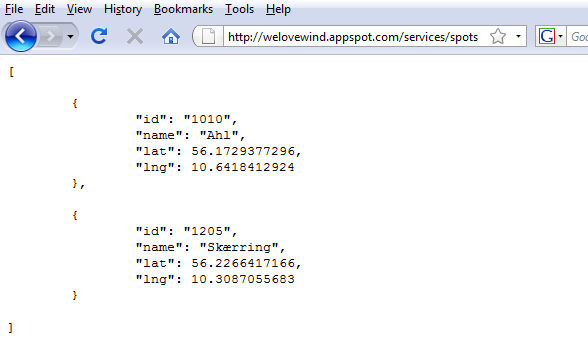
\includegraphics[width=11cm]{./Figures/spots_service}
%        \rule{\textwidth}{0.005in}
	\caption{Spots Service}
	\label{fig:spots_service}
\end{figure}

\section{Further GAE prerequisites}
This section presents GAE prerequisites for later sections. The reader can skip
the section for now and revisit it when the prerequisites are used in later
sections.

\subsection{Unique Properties}\label{sec:unique_props}
In the datastore there is no built-in option that enforces unique properties on
the models. Per design there is only one unique property namely the key of the
model. This leaves two possibilities for implementing unique constraints:

\begin{enumerate}
  \item simulate unique properties in Python\footnote{An example of a Python
  programmatic implementation of unique properties is available at:
  \url{http://appengine-cookbook.appspot.com/recipe/get-or-insert-entity-by-unique-properties/}};
  or
  \item incorporate the unique property in the key name.
\end{enumerate}

Simulating unique properties results in a fairly clean solution, however, it has
the huge flaw that there is no possible way of ensuring that the properties are
indeed unique since they are simulated. This is a problem if the solution is
applied in a concurrent environment and uniqueness guarantees are essential. The
second solution is obviously a solution to a recurring problem and we describe
this in the following.

As mentioned, the datastore ensures exactly one unique property per instance: the
key name of the instance. The Datastore API provides a transactional method on
models which either gets or inserts an instance based on the key name. We use the
method to ensure uniqueness by incorporating the unique constraints in the
keyname.

Listing~\ref{lst:unique_props_keyname} shows the implementation of unique
properties for the \verb|Forecast| weather data class. It is based on the concept
that a forecast point only should have one forecast for each time delta (the
difference between calculation time and forecast time). The delta is incorporated
into the key name to ensure the uniqueness.

The class method \verb|key_name| returns the unique key name to use for the
entity; the key name is the URI of the forecast resource. The method is used in
\verb|update_or_insert|, which as the first step calls it to get the key name
from the given arguments. The key name is used as input to \verb|get_or_insert|
that gets or creates a forecast with the specified time delta and forecast point,
now incorporated in the key name.

Instead of only getting an entity when the entity exist the authors
implementation updates the entity both when entities are updated and created. To
find out whether the entity exists a \verb|is_new| key word is passed to the
entity model. Since the key word is used only when the entity is unsaved the
property is only set to \verb|True| in this case.


\begin{lstlisting}[label=lst:unique_props_keyname,caption=Forecast with unique properties]
class Forecast(AbstractWeatherData):
  
  def __init__(self, is_new = False, **kwds):
    self.is_new = is_new
    super(Model, self).__init__(**kwds)

  (...)

  @classmethod
  def key_name(cls, calculation_time, forecast_time, forecast_point):
    time_delta = wlwtime.timeDifferenceInHours(calculation_time, forecast_time)
    owner = forecast_point.key().name()
    return '%s/forecasts/time_delta/%s' % (owner, time_delta)

  @classmethod
  def update_or_insert(cls, calculation_time, **kwds):
    '''Update or insert forecast weather data.
          
    Args:
      calculation_time: forecast calc. time (datetime).
      **kwds: Key word arguments to pass to the instance and 
        update / init the value of.
          
    Returns:
      Updated / new instance.
    '''
    key_name = Forecast.key_name(calculation_time, 
             kwds['time'], kwds['forecast_point'])
    entity = super(Forecast, cls).get_or_insert(key_name, is_new=True, **kwds)
    if not entity.is_new:
      for prop in kwds.keys():
        setattr(entity, prop, kwds[prop])
      entity.put()
    return entity
\end{lstlisting} 

\subsection{Pagination}\label{gae:pagination}
Pagination is the process of splitting up content into several resources. The GAE
limits the number of returned results of a query and restricts the duration of a
request. Because of the restrictions pagination is a must have.

Django comes with a built-in paginator class that handles pagination. The
paginator takes a complete list of objects and provides methods to get specific
pages. However, since the class takes a list of all the objects that should be
paginated it causes a slowdown as more and more objects are in the list; in
addition, since the datastore is limited to a result set of 1000, the paginator
is not able to access list objects beyond the limit.

The author's initial (un-scalable) solution was a slightly changed version of the
paginator that only retrieved objects that belonged to the current page plus one
more object. The extra object is used to evaluate whether the current page has a
next page. The new paginator instead of taking a list of objects, takes a query
as argument. The paginator then puts the relevant filters on the query object to
retrieve only the objects needed for the page requested plus the additional
entity to evaluate whether the page has an additional page. The modified
paginator fetches objects with the following query:
\begin{verbatim}
objects =  query.fetch(limit=per_page + 1,
                       offset=(self.page_number-1) * per_page)
\end{verbatim}
This query is un-scalable. Specifying an offset merely chops off entities in the
result set, however, the entities are still fetched from the datastore. That the
offset argument is provided is just confusing.

The only way to do scalable pagination is paging based on an indexed property and
limiting the number of entities. Following pages continues from the last value
(in the previous page) in terms of the ordering using an in-equality filter on
that property. We put it to use in Section~\ref{sec:models}.


\subsection{Timezones}\label{sec:gae_tz}
All times in the datastore are stored in Coordinated Universal Time (UTC). When
displaying times to the user the application should convert the UTC times to the
local times. The easiest way to convert between UTC and the timezone of the user
is by using JavaScript. However, JavaScript is not always available and then a
conversion on the server is needed.

Converting between timezones on the server is complicated since Python does not
come with logic to handle the different timezones. It merely provides an abstract
interface. What is needed is a complete database of the politically decided
timezone offsets and daylight saving times. The tz database, or Olson Timezone
database, is a continuously maintained database of timezone info. In Python the
\verb|pytz|\footnote{\url{http://pypi.python.org/pypi/pytz/}} module wraps the tz
database and provides access to the Olson database. The \verb|pytz| module is not
included in the Python Standard Library.

\verb|pytz| includes over 500 hundred files. The GAE has a restriction of 1000
uploaded files; the limit is quickly crossed when including pytz. All files
except four are binary timezone definitions belonging to the \verb|tz|
database. A blog entry\footnote{\url{http://takashi-matsuo.blogspot.com/2008/07/using-newest-zipped-pytz-on-gae.html}}
describes how to circumvent the problem by zipping all the timezone files, and
include logic to unzip them during runtime.

The GAE provides a distributed memory cache -- memcache -- which is a distributed
hash table. Unzipped timezones are obvious subjects for caching in the
distributed memory. Saving timezones in the memcache avoids the overhead in
unzipping data from the \verb|tz| database repeatedly.

Listing~\ref{lst:pytz} shows the single method in \verb|pytz| we overwrite to
incorporate the two changes: the changed method reads timezone definitions from
the zipped archive of timezones \verb|zoneinfo.zip|, and caches the result in the
memcache. The code is based on an example from the Google App Engine Cookbook
\footnote{\url{http://appengine-cookbook.appspot.com/recipe/caching-pytz-helper/}}.

\begin{lstlisting}[caption=Altered pytz,label=lst:pytz]
def open_resource(name):
    """Open a resource from the zoneinfo subdir for reading.

    """
    import zipfile
    from cStringIO import StringIO
    name_parts = name.lstrip('/').split('/')
    for part in name_parts:
        if part == os.path.pardir or os.path.sep in part:
            raise ValueError('Bad path segment: %r' % part)
    cache_key = "tzinfo/%s/%s" % (OLSON_VERSION, name)
    zoneinfo_contents = memcache.get(cache_key)
    if zoneinfo_contents is None:
        zoneinfo = zipfile.ZipFile(os.path.join(os.path.dirname(__file__), 
            'zoneinfo.zip'))
        zoneinfo_contents = zoneinfo.read(os.path.join(
            'zoneinfo', *name_parts).replace('\\','/'))
        memcache.add(cache_key, zoneinfo_contents)
    return StringIO(zoneinfo_contents)
(...)

# We don't need this, since we are including all tzinfo files
#all_timezones = [
#        tz for tz in all_timezones if resource_exists(tz)]

\end{lstlisting}

\verb|pytz| iterates through all timezone files when it is initialized, checking
whether every timezone file exist, we remove this as we have included the whole
tz database; avoiding the latency of unzipping over 500 files everytime the
server is started. The removed code is also shown in Listing~\ref{lst:pytz}.

With \verb|pytz| in place we are armed to convert between
timezones. Listing~\ref{lst:utc_to_local} shows how to convert from the times
stored in the datastore, UTC, to a local timezone. Datetimes stored in the datastore
does not have timezone information in them; before converting to local time it
must be added. After the datetime is enriched with timezone information it is
converted to local time with \verb|astimezone(tz)|: the function adjusts a
datetime according to the given timezone.

\begin{lstlisting}[caption=Converting datastore time to localtime,label=lst:utc_to_local]
>>> from pytz import timezone
>>> from datetime import datetime
>>> def local_time(utc_dt, tz_string):
...     utc = timezone('UTC')
...     utc_dt = utc_dt.replace(tzinfo=utc)
...     tz = timezone(tz_string)
...     return utc_dt.astimezone(tz)
...
>>> utc = datetime.utcnow()
>>> utc
datetime.datetime(2009, 5, 5, 6, 30, 53, 793000)
>>> lt = local_time(utc, 'Europe/Copenhagen')
>>> lt
datetime.datetime(2009, 5, 5, 8, 30, 53, 793000, tzinfo=<DstTzInfo 'Europe/Copenhagen' CEST+2:00:00 DST>)
\end{lstlisting}

\verb|pytz| is put into action in Section~\ref{sec:models}, where we also
describe how to get the relevant timezone string, e.g.,
\verb|'Europe/Copenhagen'|.

%% \section{Cron jobs}
%% Long running requests on GAE is aborted, and a message is sent to the
%% user. This poses a problem for the welovewind webapp, as the app has to
%% fetch data at several external resources. Obviously, this can't be done
%% be fetching external data from the source every time it's
%% needed. Instead we keep track of when to fetch new data and insert this
%% into the datastore.

%% "spawn a sub-process or thread. A web request to an application must be handled in a
%% single process within a few seconds. Processes that take a very long time to respond
%% are terminated to avoid overloading the web server."


%% Then sign up for one of those web-site 
%% monitoring services that ping your website to see that it's alive

%% \url{http://schedulerservice.appspot.com/about}

%%\section{Testing}

%%\section{Comet, AJAX Push}

%%\section{Comparison to similar offerings}

\section{Summary}
In this chapter we have presented the GAE and the Web application framework,
Django. GAE and Django is used in the rest of the dissertation as the basis upon
which we shall build several elements that will support the aspiration of assisting
wind- and kitesurfers. The chapter also presented GAE solutions to the common
problems of pagination, unique properties of data models, and conversion of times
to another timezone.


\part{The Web Services}
%% The Web Service is the corner stone of the application. The Web Service is used
%% both to keep weather data up to date, from cron jobs running at external
%% locations, and in addition, to back the front-end of the application.

%% The problem domain investigated in Section~\ref{sec:user_and_task} is the
%% foundation for deriving the resources of the Web Service. After describing the
%% resources and their representations, in Chapter~\ref{chap:resources}, we dig into
%% how to sort out subtleties regarding realizing the data in the resources.

%% Chapter~\ref{chap:gae_ws} and~\ref{chap:ws_daimi} describe the implementation of
%% the Web Service. Because of restrictions in the GAE the Web Service consists of
%% two Web Services: one located at the GAE, and one located at DAIMI. The former
%% chapter describes the implementation of the Web Service at the GAE; and, the
%% latter describes the implementation of the Web Service at DAIMI.

%% While reading this part the reader might wonder where the data in the services
%% will come from. The data in the two Web Services are put in there by Web Service
%% clients described in the next part of the thesis.
\chapter{Resources and their Representations}\label{chap:resources}
Based on the scenarios in Section~\ref{sec:scenarios} we derive the resources for
our Web Service which is the corner stone of the application. The nouns of
the scenarios define the resources in the Web Service: spots, weather stations,
and forecasts. All representations of the resources are in the JSON format.

In the sections about resources we summarize the resources in what we call a
resource view. Together the views describe the resource view of the software
architecture from the resource viewpoint. The concept of views and viewpoints is
presented in \citep{sa:arch_desc}. 
%
\begin{definition}\label{def:resource_viewpoint}
The \emph{resource viewpoint} on the software architecture is concerned with what
resources the system contains and what parts of the uniform interface they expose.
\end{definition}

\section{Spots}
A spot is a geographical point where people wind- and kitesurf. A point is
naturally encoded by latitude and longitude. All spots have a name and
information about its wind directions suitable for surfing; we denote the
property of a spot being apt for surfing (suitable wind in a suitable direction)
as surfability. The directions of surfability are described in a wind
diagram that captures in which directions -- North, North-East, East, etc. -- the
spot is surfable.

Listing~\ref{lst:spotsrep} shows an example of the representation of the spots
resource. The resource is a JSON object that among others contains the following
fields:
\begin{itemize}
  \item \verb|next| is an indicator for \textit{\gls{gls:pagination}}.
  \item \verb|items| a list containing individual spots.
  \item \verb|uri| the URI of the concrete spot.
  \item \verb|forecast_point| the nearest point where forecasts for the spot are calculated for. 
\end{itemize}

The spots resource is the first of three list resources. The list resources have
the same structure: a \verb|next| field which is the URI of the next page or the
empty string if the page is the last and an items field containing the concrete
items. The uniform structure will come in handy when retrieving resources in the
clients.

Spots are connected to the nearest forecast point (soon presented) and the
individual spots, hereby satisfying connectedness.

\begin{lstlisting}[caption=Spots representation, label=lst:spotsrep]
 {
    "next": "",
    "items": [
     {
       "name": "Ahl",
       "country_code": "dk",
       "lat": 56.1729377296,
       "lng": 10.6418412924,
       "wind_diagram": {
	 "S": "YES",
	 "SW": "YES",									
	 "W": "YES",			
	 "NW": "YES"
       },
       "uri": "/spots/ahl/",
       "forecast_point": "/forecasts/56.0,10.5/"
     },
     (...)
   ]
}

\end{lstlisting}
In addition to paging, for performance reasons the list of spots must be subject
to different filters reducing the total number of spots returned; there must
exist filters to reduce the list to
%
\begin{enumerate}
  \item only spots in the proximity of a geographical point; and
  \item only spots in a certain country.
\end{enumerate}
%
The preceding representation is served to the client. We now turn to the
representations sent from the client. 

Spots are created by any user in the system. The application receives concrete
spot resource representations to either create or update spot resources.  The
representation of spots accepted from the client at the server is different than
those sent to the client. The representations accepted from the client are in the
format that browsers submit data in: the official name is
\verb|application/x-www-form-urlencoded| \citep[sec.17]{w3:HTML}, we denote it
uri-encoding from now on. The difference in format is because we rely on Django
forms on the server side. Django forms gives much for free, including validation
of fields, error messages to return to the user, and acceptance of
uri-encoded data directly. A uri-encoded spot representation looks like the
following:
\begin{verbatim}
name=Ahl&lat=56.172&lon=10.641&country_code=dk&S=YES
\end{verbatim}

\begin{table}[htbp]
\centering
\setlength\extrarowheight{3pt}
\begin{tabularx}{\textwidth}{l X}
\toprule
Resource URI    & Action\\\midrule
\verb|/spots/|  
                & \verb|GET| all spots at page 1\\
\verb|/spots/{country_code}/|
                & \verb|GET| all spots in a certain country\\
\verb|/spots/|  
                & \verb|POST| a new spot\\
\verb|/spots/{spot name}/|
                & \verb|PUT| a new representation of an existing spot\\
\verb|/spots/{spot name}/|
                & \verb|DELETE| an existing spot\\
\bottomrule
\end{tabularx}
\caption{Resource view of spot resources}\label{tab:spot_resources}
\end{table}
An overview from the resource viewpoint of the resources discussed in this
section is given in Table~\ref{tab:spot_resources}. The URIs support the naming
conventions stated in \citep[p.117-118]{rest:webservice}; this means,
\begin{itemize}
 \item \verb|/| indicates a \verb|parent/child| resource hierarchy;
 \item \verb|,| or \verb|;| indicate no hierarchy. The former indicates that the
 order is significant, e.g., the latitude and longitude pair \verb|56.0,10.5|,
 whereas the latter indicate that the order is insignificant. Inputs that
 conceptually are arguments to an algorithm are indicated with query parameters.
\end{itemize}

\section{Weather Stations}\label{sec:res_weather_stations}
A weather station is a place where observations are created. Observations
consist of a time, a wind velocity measurement, and a temperature
measurement. The application currently has three resources for live weather data
DCA, DMI, and WB.

\subsection*{DCA and DMI}
Live weather data -- wind speed and gust, temperature, and direction measurements
-- are available at DCA (of the west coast in Jutland) and DMI (most regions in
Denmark). 

The latest observation is interesting and is exposed as a resource. In addition,
it is relevant to know whether the wind picks up or slacks down based on the last
observations. Therefore a list of weather observations belonging to a specific
station is a resource. The latest observations is incorporated into the weather
stations resource; the reason is that the last observation is needed in most
cases, and this is not the case for the rest of the observations.

Listing~\ref{lst:weather_stations} shows an example of the representation of
weather stations. The resource is a JSON object that among others contains the
following fields:

\begin{itemize}
  \item In the JSON list, \verb|items|, the \verb|uri_extern| field specifies the
URI of the weather station at the external location: the external page to link
to. The page to scrape is identified by \verb|uri_scrape|.
  \item The last two fields in the list are links to the weather station and its
  observations respectively, thereby satisfying the constraint of connectedness.
  \item The timezone field is used to convert the UTC observation time stored in
  the database to the time where the weather station is located when JavaScript
  is not available.
\end{itemize}

\begin{lstlisting}[caption=Weather stations representation, label=lst:weather_stations]
{
  "next": "/api/weather_stations/?geohash_offset=swgv3sxf003p"}  
  "items": [
    {
      "name": "Skagen", 
      "lat": 57.723952722299998, 
      "lon": 10.5997467041016, 
      "timezone": "Europe/Copenhagen", 
      "type": "DCAWeatherStation", 
      "latest": {
        "direction": 242.90000000000001, 
        "icon": "/images/wind_arrows/SW_4to6.png", 
        "speed": 5.9000000000000004, 
        "temp": 13.0, 
        "time": "2009-06-19T12:00:00"}
      },
      "uri": "/api/weather_stations/dk/skagen/",
      "uri_extern": "http://www.kyst.dk/sw3029.asp", 
      "uri_observations": "/api/weather_stations/dk/skagen/observations/", 
      "uri_scrape": "http://www.kyst.dk/custom_asp/defaultjs.asp?id=3003&targetStation=1100"
    },(...)
  ]
}
\end{lstlisting}

The representation for observations for a specific resource is a list of objects
containing weather data; an example is shown in Listing~\ref{lst:obs_res}. The
\verb|time| field indicates the time of the observation in UTC time, the
\verb|speed| and \verb|gust| field indicates the speed in \verb|m/s|, the
\verb|direction| field is the direction in degrees where the wind is blowing
from, and the \verb|icon| field is a link to a representative direction and speed
icon. 

\begin{lstlisting}[label=lst:obs_res,caption=Observations representation]
{
  "owner": "/weather_stations/dk/skagen/",
  "page": 1,
  "has_next": true,
  "items": [
    {
      "direction": 242.9, 
      "icon": "/images/wind_arrows/SW_4to6.png", 
      "speed": 5.9, 
      "temp": 13.0, 
      "time": "2009-06-19T12:00:00"
    },
    (...)
    ]
}
\end{lstlisting}

\subsection*{WeatherBug}
DCA and DMI produce weather observations only for Denmark; additional resources
are needed.

WeatherBug provides an API to access weather information worldwide. We use the following
functions from the API:
\begin{itemize}
  \item retrieve an XML list of stations in the proximity of a latitude and longitude; and,
  \item retrieve an RSS feed of live weather data for a specific weather station.  
\end{itemize}
Representations of the weather resources are obviously already created. The
existing representations, at first sight, open the option to completely bypass
the application server and let JavaScript retrieve the relevant weather data
directly from WeatherBug. The representations, however, are not in JavaScript
format which makes it impossible to load data directly into browser
clients because of the same origin policy described in Section~\ref{sec:json}.

Another option is storing the data on the GAE server and update the content as it
becomes stale. This approach is the only option that serves data fast enough and
is therefore chosen. Following the approach weather stations are subject to
frequent updates of observations. Updates are uploaded from a Web Scraper located
at an external machine. We expose the \verb|POST| method of the observations
resource to post observations to since the concrete URI of the posted resource is
unknown. The observation representation accepted from the client is in JSON
format, and is just a single item of the observations list shown in
Listing~\ref{lst:obs_res}. 

We use the same representation for WeatherBug stations as for DCA and DMI weather
stations. An overview of the resources is given in Table~\ref{tab:ws_resources}. 

\begin{table}[htbp]
\centering
\setlength\extrarowheight{3pt}
\begin{tabularx}{\textwidth}{l X}
\toprule
Resource URI    & Action\\\midrule
\verb|/weather_stations/|  
                 & \verb|GET| all weather stations\\
\verb|/weather_stations/{country_code}/|
                 & \verb|GET| all weather stations in a certain country\\
\verb|/weather_stations/{id}/observations/|
                 & \verb|GET| all weather observations\\
\verb|/weather_stations/{id}/observations/|
                 & \verb|POST| a new weather observation\\
\bottomrule
\end{tabularx}
\caption{Resource view of weather station resources}\label{tab:ws_resources}
\end{table}

\section{Forecast Points}\label{sec:res:forecast_points}
A forecast point is a specific point on the Earth where forecasts are calculated
for. A forecast is a prediction of the weather at some specific time for a
specific forecast point.

A natural source for forecasts is DMI; however, their forecast data is
unavailable and they have no interest in joining in on a collaborative
project. The National Oceanic Atmospheric
Administration\footnote{\url{http://www.noaa.org/}} (NOAA) in the US, however, by
law puts weather data into the public
domain\footnote{\url{http://www.weather.gov/disclaimer.php}}. This means use of
their data is allowed in almost any context, and that we can be certain that the
service continues.

NOAA produces many highly detailed forecast for the US, and in addition global
forecasts using the Global Forecast System\footnote{Info about the GFS model
\url{http://www.emc.ncep.noaa.gov/modelinfo/index.html}} (GFS). The forecasts are
made four times daily at 00, 06, 12 and at 18 o'clock UTC. At these four times
detailed forecasts are calculated for the next 48 hours with a three hour
interval between them; actually there are forecast with a longer prediction in
the future but these are of decreasing detail. The most detailed GFS forecasts
produced at NOAA are produced at a degree of 0.5�.

A note on accuracy: the earth has latitudes in the interval [-90�;90�]. This
gives a total of 360 points along \textit{\gls{gls:meridian}}s that are subject
for forecasts. Longitudes are values in the interval [-180�;180�]. This yields
720 points. Looking at a map we can see that in this resolution, e.g., Aarhus and
Skanderborg probably are associated with the same grid location.

Detailed NOAA GFS forecasts are located at
\url{http://nomad3.ncep.noaa.gov/pub/gfs/rotating-0.5/}. In the directory there
are three important types of files:
%
\begin{enumerate}
  \item Forecasts in GRIB2 format named \verb|gfs.t{TT}z.pgrb2f{XX}|;
  \item inventories for forecasts named \verb|gfs.t{TT}z.pgrb2f{XX}.inv|; and
  \item descriptor files for a specific run named \verb|gfs_t{TT}z.ctl|; 
\end{enumerate}
% 
In the above \verb|TT| is the time of the calculation and \verb|XX| is a delta in
hours to add to the time of calculation to get the time of the prediction. In the
descriptor file all the fields in the forecasts are defined. For now we are
interested in the wind forecast which is given by a vector split up into a \verb|u| and a
\verb|v| component of the wind 10 meters above the ground. In addition, we are
interested in the temperature forecast near the surface given by a single field
where the value is reported using the Kelvin scale. The value of the fields is
retrieved by, e.g., \verb|wgrib2| introduced in Chapter~\ref{chap:forecasts}.

\begin{lstlisting}[caption=Forecast points representation, label=lst:forecast]
{
  "next": "",
  "items": [{
      "lat": 36.5, 
      "calculation_time": "2009-07-01T06:00:00", 
      "lon": 29.0,
      "uri": "/api/forecast_points/36.5,29.0/", 
      "forecasts": [{
          "direction":252.53999999999999, 
          "icon": "/images/wind_arrows/W_6to8.png",
          "speed":6.5300000000000002, 
          "temp": 27.050000000000001, 
          "time": "2009-07-01T12:00:00"},
        (...)
      }
    (...)
  ]
}

\end{lstlisting}

Listing~\ref{lst:forecast} shows the representation of forecasts for a specific
point. It contains the time of forecast calculation, and the forecasts. An
overview of the resources is given in Table~\ref{tab:for_resources}.
\begin{table}[htbp]
\centering
\setlength\extrarowheight{3pt}
\begin{tabularx}{\textwidth}{X X}
\toprule
Resource URI    & Action\\\midrule
\verb|/forecast_points/|  
                & \verb|GET| all points\\
\verb|/forecast_points/{lat},{lon}/|
                & \verb|GET| a forecast point representation\\
\verb|/forecast_points/{lat},{lon}/|
                & \verb|PUT| a new forecast point representation\\
\bottomrule
\end{tabularx}
\caption{Resource view of the forecast points resources}\label{tab:for_resources}
\end{table}
Updates of a point's forecasts are supported by exposing the \verb|PUT| method of
the uniform interface. The representation accepted is in the same JSON format.

In comparison to weather station resources, forecast point resources have no
weather data resources belonging to it. Forecast point resources consist of both
forecast point information and all the forecasts. The reason for deviating is
that all weather data of the forecast point belong to a specific calculation time
of the forecast point making it more natural to think of all the content as a
single resource.

\section{Sorting out the resource requirements}\label{sec:proximity}
In the last section we pointed out the resources in the Web Service, not how to
process the content in them. Filtering points on a proximity basis is
non-trivial. This section reviews our solution.  

The application will eventually contain a huge data set: spots, weather stations,
forecast points, etc. Returning the whole data set is infeasible in terms of
latency at the client.  In addition, we have a
\textit{\gls{gls:location_based_service}} requirement. To sum up, filtering by
location reduces the data set, and increases the relevancy of the data
set. Therefore, the application needs a filter on points which returns a subset
of points in the proximity of a certain place.

Filtering on proximity sounds like a rather easy problem but it is not. To limit
the result set, in a usual database several inequality filters are applied to the
latitude and longitude values creating a bounding box. As mentioned in
Section~\ref{sec:queries}, the datastore can only apply inequality filters on a
single property; a bounding box demands two: an index on latitude and an index on
longitude. Listing~\ref{lst:proximity_query} shows a dysfunctional GAE query that
one could think would solve the problem.

\begin{lstlisting}[label=lst:proximity_query,caption=Dysfunctional GAE bounding box query]
>>> from wlw.models import Spot
>>> from google.appengine.ext import db
>>>
>>> point_1 = db.GeoPt(lat=50, lon=-10)
>>> point_2 = db.GeoPt(lat=60, lon=0)
>>> q = db.Query(Spot) \
...   .filter('point >', point_1) \
...   .filter('point <', point_2)
>>> for s in q:
...    print 'spot: %s \npoint: (%s)' % (s.key().name(), s.point)
...
spot: ahl
point: (56.1729377296,10.6418412924)
\end{lstlisting}

The filters in the query apparently set up a bounding box, but, because of the
inequality filter restriction the query ignores the longitude boundary given by
the \verb|GeoPt| property, and only filters on the latitude. The problem results
in GAE returning \textit{all} spots that lie within the given latitudes, in this
case only one: Ahl.

We present two approaches to the problem, where the first is an obvious solution,
but it does not scale as the data set gets large. The other, is a scalable
solution based on geohash.

\subsection{Calculating proximity points with haversine}
Finding proximity points is possible by first calculating the distance between a
reference point and all other points; afterwards, filtering out points over a
certain threshold distance to the reference point.

In the following we assume the Earth is a sphere ignoring the fact that best
approximation is an oblate spheroid\footnote{http://en.wikipedia.org/wiki/Earth}.

%
A great circle is a circle on a sphere which cuts the sphere into two equally
sized halves, i.e, the circle has radius equal to the radius of the sphere and
the same center as the sphere. An area on the sphere bounded by three arcs of
great circles that do not all have a common point is called a spherical
triangle. The (shortest) distance between two points on a great circle is the
shortest possible distance between the two points, since the arc on the great
circle is the arc with the smallest deviation from a straight line.  Looking at
Figure 5.1, which shows a spherical triangle, the arc c along the great circle is
the shortest distance between A and B. 
%
\begin{figure}[htbp]
  \centering
  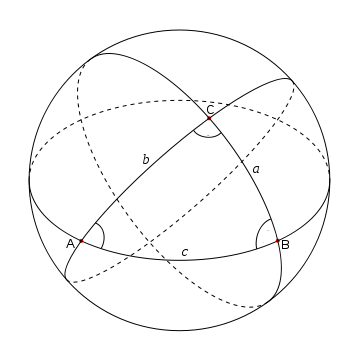
\includegraphics[width=8cm]{./Figures/spherical-triangle2}
  \caption{Illustration of a spherical triangle}
  \label{fig:spherical_triangle}
\end{figure}
In a spherical triangle in a unit sphere the law of cosines relates the sides and
angles of the triangle, in the following way:
%
\begin{theorem}\label{thm:law_of_cosines}
Spherical law of cosines \citep[p.130]{mat3}
\begin{equation}
  cos(c) = cos(a)cos(b) + sin(a)sin(b)cos(C) 
\end{equation}
\end{theorem}
%
Isolating $c$ in the formula gives the distance between the points $A$ and
$B$. However, when $c$ (the distance) is small rounding errors are stated to be
significant \citep{gis:haversine,wiki:haversine,haversine:sinnott}, therefore,
instead the haversine formula is used \citep{haversine:sinnott}. The formula is
based on the haversin function, defined as:
%
\begin{equation}
  haversin(\theta) = sin^2(\frac{\theta}{2})
\end{equation}
%
The following identity between $cos$ and $haversin$ exists:
%
\begin{align}
  cos(2\theta) &= 1 - 2sin^2(\theta) \notag\\
  \tag{double-angle formula \citep[p.A23]{math:stewart}}\\
  cos(\theta) &= 1 - 2sin^2(\frac{\theta}{2}) = 1 - 2haversin(\theta) \label{eq:rel_cos_hav}
\end{align}
%
We now derive the law of haversines from the spherical law of
cosines. Substituting $cos$ with $haversin$ using (\ref{eq:rel_cos_hav}) in the law
of cosines, we get:
%
\begin{align}
  1 - 2haversin(c) &= cos(a)cos(b) + sin(a)sin(b)(1 - 2haversin(C))  \notag\\
  1 - 2haversin(c) &= cos(a-b) - 2sin(a)sin(b)haversin(C) \notag\\% cos(a-b) substitue with haversine \\
  \tag{Using the subtraction formulas \citep[p.A23]{math:stewart}}\\
  1 - 2haversin(c) &= 1 - 2haversin(a-b) - 2sin(a)sin(b)haversin(C) \notag\\
  \tag{Substituting $cos$ with $haversin$}\\
  2haversin(c) &= 2haversin(a-b) + 2sin(a)sin(b)haversin(C) \notag\\
\end{align}

\begin{theorem}
The law of haversines
\begin{equation}
    haversin(c) = haversin(a-b) + sin(a)sin(b)haversin(C) \notag
\end{equation}  
\end{theorem}
%
We note that $a$, $b$, and $c$ given in radians are equal to the length of the
arcs, since we are working on a unit sphere. Now let $C$ be placed on the North
Pole, then by definition its latitude is 90� or in radians $\frac{\pi}{2}$. Then,
the length of the arcs $a$ and $b$ are:
\begin{align}
  a &= \frac{\pi}{2} - B_{lat} \notag\\
  b &= \frac{\pi}{2} - A_{lat} \notag
\end{align}

%
Let $\Delta lat$ and $\Delta lon$ be the latitude and longitude differences between
$A$ and $B$ respectively, then since,
\begin{equation}
  sin(\phi) = cos(\frac{\pi}{2} - \phi) \label{eq:sin_cos}
\end{equation}
we have
\begin{equation}
  haversin(c) = haversin(\Delta lat) + cos(a_{lat}) * cos(b_{lat}) * haversin(\Delta lon)
\end{equation}
%
In the general case for a sphere with arbitrary radius the unit circle distance
$c$ is related to the real distance $d$ on the sphere by: $c = \frac{d}{radius}$  
%
\begin{theorem}
The haversine formula
\begin{equation}
  haversin(\frac{d}{radius}) = haversin(a_{lat}-b_{lat}) + cos(a_{lat}) * cos(b_{lat}) * haversin(b_{lon}-a_{lon}) \notag
\end{equation}
\end{theorem}
%
By isolating $d$ the distance is found:
\begin{equation}
sin(\frac{d}{2R}) = \pm \sqrt{haversin(\Delta lat) + cos(a_{lat}) * cos(b_{lat}) * haversin(\Delta lon)} \label{eq:dis1}
\end{equation}
\begin{equation}
sin(\frac{d}{2R}) = \sqrt{haversin(\Delta lat) + cos(a_{lat}) * cos(b_{lat}) * haversin(\Delta lon)} \label{eq:dis2}
\end{equation}
\begin{equation}
\frac{d}{2R} = arcsin(\sqrt{haversin(\Delta lat) + cos(a_{lat}) * cos(b_{lat}) * haversin(\Delta lon)}) \label{eq:dis3}
\end{equation}
\begin{equation}
d = 2R*arcsin(\sqrt{haversin(\Delta lat) + cos(a_{lat}) * cos(b_{lat}) * haversin(\Delta lon)}) \tag{the distance formula}  
\end{equation}
\\\\ In~(\ref{eq:dis3}) $arcsin$ returns the value of $\frac{d}{2R}$ in the
interval $[0,\frac{\pi}{2}]$. There is also a solution to (\ref{eq:dis2}) in
$[\frac{\pi}{2},\pi]$ but this solution is not relevant since we are interested
in the value of $\frac{d}{R}$ in $[0,\pi]$.

\subsubsection{Distance formula in Python}
The distance formula is easily implemented in Python, shown in
Listing~\ref{lst:haversine}. An example of calculating the distance between two
points is shown in Listing~\ref{lst:haversin_applied}.
\begin{samepage}
\begin{lstlisting}[caption=Python implementation of distance calculation using the haversine formula,label=lst:haversine]
from math import sin, atan2, cos, sqrt, pi

earth_radius = 6371
radian = pi / 180

def distance(point1, point2):
    '''Calculates the distance between two points, using the haversine formula.
    '''
    lat_a, lon_a = to_radians(point1)
    lat_b, lon_b = to_radians(point2)
    dlon = lon_b - lon_a
    dlat = lat_b - lat_a

    haversin_c = (sin(dlat/2))**2 + cos(lat_a) * cos(lat_b) * (sin(dlon/2))**2 

    # unit sphere distance
    c = 2 * asin(sqrt(haversin_c)) 

    distance = earth_radius * c
    return distance

def to_radians(point):
    '''Convert to radians.
    '''
    lat = point.lat * radian
    lon = point.lon * radian
    return lat, lon
\end{lstlisting}
\end{samepage}

\begin{samepage}
\begin{lstlisting}[caption=Calculating the distance between Aarhus and Aalborg,label=lst:haversin_applied]
>>> import geo,math
>>> class Point:
...     def __init__(self,lat,lon):
...             self.lat = lat
...             self.lon = lon
...
>>> aarhus = Point(56,10)
>>> aalborg = Point(57, 10)
>>> geo.distance(aarhus, aalborg)
111.12511347447912
\end{lstlisting}
\end{samepage}

\subsubsection{Why haversine? A small experiment}
We derived haversine based on the statements that using the spherical cosines
relation to calculate distance would cause significant rounding errors with small
distances. What is small in a modern context? In order to reason about this we
have implemented the direct approach to the distance calculation as well and
compared it with distance calculation based on the haversine formula.

\begin{table}
\centering
\begin{tabularx}{\textwidth}{l l l l l}
\toprule
Point       & Point                & Haversine Distance (m)& Cosines Distance (m) \\\midrule
(56.0,10.0) & (57.0,10.0)          & 111125.113474    & 111125.113474   \\
(56.0,10.0) & (56.0000009537,10.0) & 0.105977166514   & 0.0948756933212 \\
(56.0,10.0) & (56.0000004768,10.0) & 0.0529885829037  & 0.0             \\
\bottomrule
\end{tabularx}
\caption{Comparing distances calculated with haversine and cosines}
\label{tab:hav_cos_comp}
\end{table}

Table~\ref{tab:hav_cos_comp} summarizes the results using Python on a 32-bit
machine. There is a maximum difference of 5 cm between the two approaches. We
conclude that the reasoning for the haversine formula is irrelevant in a modern
context for most distance calculations on the Earth. Since we have derived
haversine we continue using it. The reader can refer to
Appendix~\ref{AppendixHaversine} for the implementations and the whole transcript
of the output of the experiment.

\subsubsection{Sorting by distance}
Sorting points by distance is easy exploiting the haversine function, as shown in
Listing~\ref{lst:haversine_sort}. Python's included \verb|sort| function can sort
using any comparator. In this case the comparator calculates the distance, using
the distance formula, between the current point and the reference point.

\begin{lstlisting}[label=lst:haversine_sort, caption=Sorting points with haversine]
def sort_by_distance(ref_point, entities):
    '''Sort entities with a point property, by distance wrt. a reference point.
    
    Args:
        entities: list of entities with a point property.
        ref_point: reference point to calculate distance from.
    Returns:
        list of entities sorted by distance. The distance is added as a member of the entity. 
    '''
    def _distance_to(entity):
        d = distance(ref_point, entity.point)
        entity.distance = d
        return d
    
    entities.sort(key=_distance_to)
    return entities
\end{lstlisting}

There is a problem with the approach using the haversine formula; it is
impossible to calculate an index in the Google datastore to support the distance
formula. Therefore finding spots within a certain distance involves a full table
scan, iterating over all spots in the database, and for each spot calculating the
distance to the reference point. 

Haversine is useful for calculating the distance between few points, but
increasing the number of points demands another approach that reduces the data
set and exploits indexing and preserves scalability. In the next section, we
present an alternative approach.

\subsubsection{Calculating proximity points with Geohash}
Geohash, invented by Gustavo Niemeyer, is an algorithm to convert between
latitude and longitude coordinates and a hash value \citep{wiki:geohash}. In
essence, geohash is just a z-order space-filling curve. Therefore a database can
benefit from a usual index on geohashed points when performing searches for
points in the proximity of each other.

Geohash is based on a custom \textit{\gls{gls:base_32}} alphabet for encoding and
decoding binary data. The custom alphabet is given by the string
\verb|"0123456789bcdefghjkmnpqrstuvwxyz"|. The index of a character in the string
is equal to the value of the character, e.g., 'z' has the associated value 31
which is $11111_2$.

Geohash supports arbitrary precision in the encoding of geographical points by
interleaving the latitude and the longitude in the bit string. A bit string such
as $b = 11111$ is decoded to a latitude longitude point as follows:

\begin{itemize}
\item Even positioned bits pertain to longitude:
\begin{math}
b_{lon} = b_0b_2b_4 = 111
\end{math}

\item Odd positioned bits pertain to latitude:
\begin{math}
b_{lat} = b_1b_3 = 11
\end{math}
\end{itemize}

\begin{figure}[htbp]
  \centering
  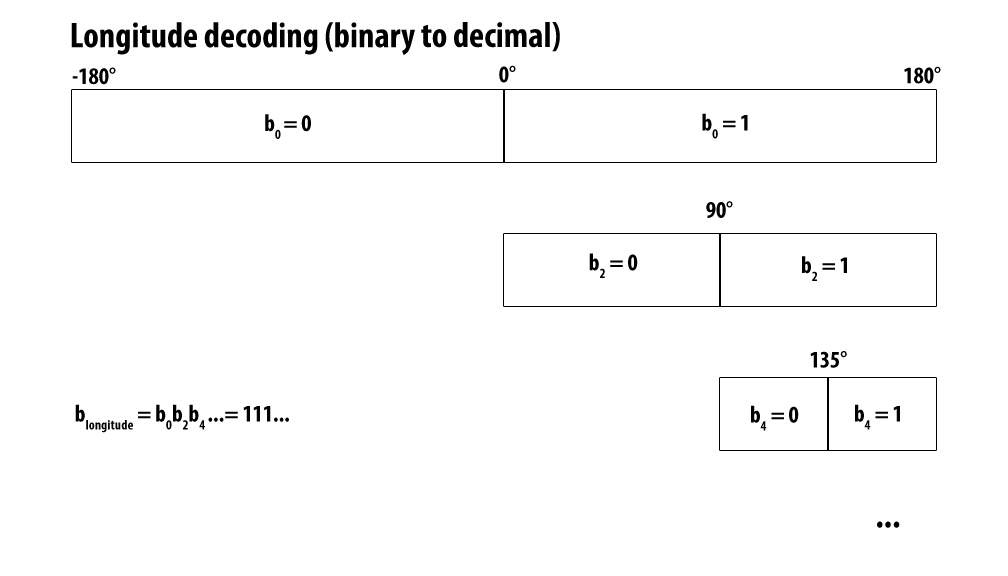
\includegraphics[scale=0.3]{./Figures/geohash_decoding_lon}
  \caption{Geohash longitude calculation}
  \label{fig:geohash_calc}
\end{figure}

Every bit in $b_{lon}$ and $b_{lat}$ halves the point's location space. When the
bit is set the upper half is chosen. The longitude of geohash 'z' is therefore
between [135�,180�], as shown in Figure~\ref{fig:geohash_calc}, and the latitude
is between [45�,90�]. All points with prefix 'z' are in this area. A specific
point is calculated by taking the mean value of the range; thus, the geohash 'z'
equals the point (67.5�, 157.5�).

There are two Python geohash implementations available: \citep{geohash:erle}
which is in the public domain and \citep{geohash:norrgard} which is licensed
under GNU Affero General Public License (AGPL)\footnote{AGPL is a somewhat more
restrictive license than GPL. A Web application based on GPL software must only
open source the software if the software running the service is distributed to
others. AGPL, in essence, demands that the software running the Web application
is open sourced also if the software is not distributed.}. The former is a bit
more advanced; it supports addition of geohashes, and has two formats for the
hash: binary and character based. The result of an addition is the minimal
bounding box of the two geohashes. An example of the usage of the first
implementation is shown in Listing~\ref{lst:geohash_example}. Note that the usual
convention of the sequence latitude and longitude is reversed to longitude and
latitude. The last line in the example shows that the implementation is buggy
when decoding hashes. We have just shown above that the point represented by 'z'
was (67.5�, 157.5�) and this is not the case here, the longitude is wrong. On the
server in the application we encode geographical points using
\citep{geohash:norrgard}.

\begin{lstlisting}[caption=Geohash example usage,label=lst:geohash_example]
>>> import geohash
>>> london_west = geohash.Geohash((-0.12,51.50))
>>> str(london_west)
'gcpuvr295zcd2'
>>> london_east = geohash.Geohash((0.12, 51.50))
>>> str(london_east)
'u10hfxr3hpy6q'
>>> world = london_east + london_west
>>> str(world)
''
>>> geohash.Geohash('z').point()
(180.0, 67.5)
\end{lstlisting}
%
Listing~\ref{lst:geohash_example} also shows a general problem with geohasing: the
property of similar prefixes of points in the proximity of each other is not
always true. The problem lies within proximity points with different prefix. Take for
instance the area just West of London, Greenwich; the hash of the western side
(bit 0 unset), has a complete different prefix than the hash of the eastern side
of Greenwich (bit 0 set) because boxes have a borderline here: namely the prime
meridian. Restricting proximity points to a certain prefix results in lost
proximity points.

\subsubsection{Lost proximity points: a solution}\label{sec:lost}
The \gls{gls:base_32} alphabet and the algorithm of geohash result in a
conceptual grid that is overlayed on the Earth, shown in
Figure~\ref{fig:geohash}. This grid is essential in solving the problem of lost
proximity points.

\begin{figure}[htbp]
  \centering
  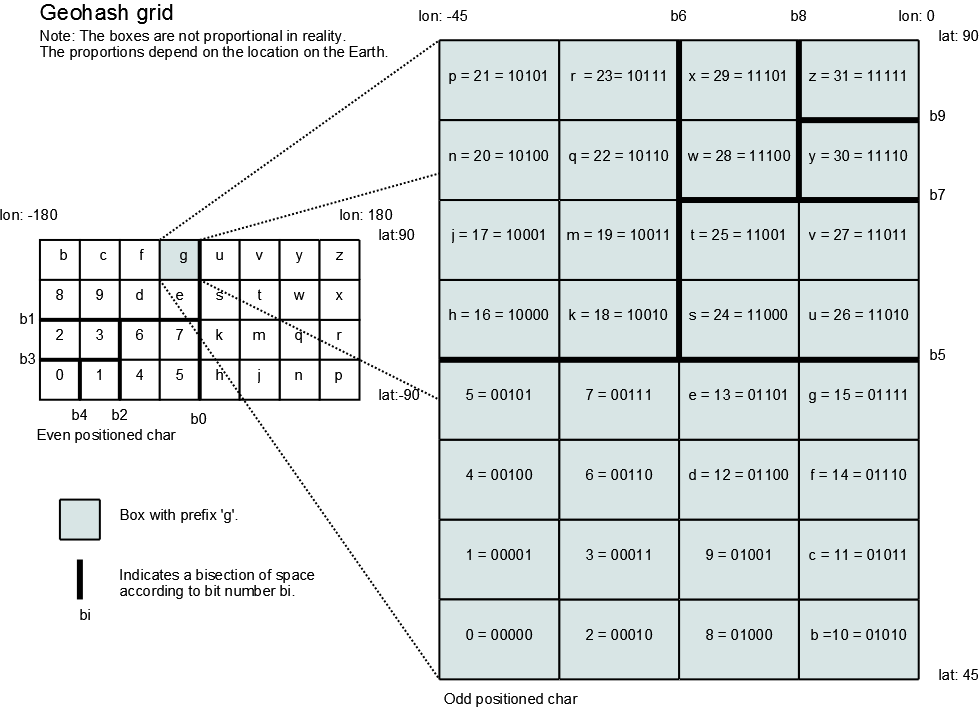
\includegraphics[scale=0.3]{./Figures/geohash}
  \caption{Cylindrical projection of Geohash grid}
  \label{fig:geohash}
\end{figure}

A solution to the proximity problem is augmenting the returned data set with
points from all the grid boxes surrounding the requested one: the neighbors
directly to the north, northeast, east, etc.

The geohash grid has a recursive structure: every char in a geohash specifies a
grid box container, and the next char in the geohash specifies a grid box within
the first grid box container, and so on. The position of the char, even or odd,
decides which of the two containers in the figure is representative for the char,
since even positioned chars begin with an even bit, and odd positioned chars
begin with an odd bit.

We have implemented a solution where the two representative grids are represented
as matrices: allowing for easy navigation to the neighbors of a grid
box. Navigating to neighbors falls into three cases:

\begin{enumerate}
  \item the neighbor is in the same container; 
  \item the neighbor is in a neighbor container; or,
  \item the neighbor is on the other side of the cylindrical projection, i.e.,
  crossing the ends of the square cylindrical projection.
\end{enumerate}
%
Locating a neighbor in the first case is easy: for all neighbors return their
geohash, which is the current geohash with the last char replaced by the char
representing the new location in the container.

Locating the neighbors in the second case is more tricky. The case is identified
by going out of bounds of the matrix. By wrapping around the indexes we identify
the new suffix of the grid box we are after, i.e., if the request is for the
Eastern neighbor of geohash 'z' the index is wrapped around to the other side
which is 'b' (in the even case). However, as we are out of bounds, we need to
zoom out and still find the eastern neighbor. Zooming out and tracking the
neighbor is equal to doing the same query on the geohash with the last char
stripped.

If the container of 'z' has an eastern neighbor the tracking succeeds and we can
return the char of the eastern container concatenated with the suffix identifying
the grid box within it, found when wrapping around. 

The third case happens when we are fully zoomed out: in this case there exist no
neighbors in the grid; however, the logical neighbor is still found by wrapping
around (this only makes sense for East-West directions). We can think of this as
connecting the ends of a square map of the world assuming it is created by a
cylindrical projection.

An excerpt of the implementation of geohash neighbors is shown in
Listing~\ref{lst:geohash_neighbor}. The main method is \verb|step_in_direction|
which returns the grid box, at the same zoom level, which is the neighbor to the
box of the given geohash in the requested direction. The function calls itself
recursively when it must zoom out to find the neighbor. Under the recursive call
it keeps the found suffix of the neighbor in the \verb|new_geohash_suffix|
argument, and when a neighbor is found the char of its grid box is concatenated
with the \verb|new_geohash_suffix| resulting in another geohash suffix. At last
the suffix if prefixed with the geohash of the current zoom level. We note that
the time used to find neighbors is in the worst case proportional to the length
of geohash (the number of times to zoom out).

\begin{samepage}
\begin{lstlisting}[label=lst:geohash_neighbor, caption=Geohash neighbors implementation]        
def neighbors(geohash):
    '''
    Calculate surrounding geohashes.
    Precondition:
        len(geohash) > 0
    Returns:
        A list of neighbors as a list of geohashes, in the order N, NE, E, SE, ...
    '''
    geohash_north = step_in_direction(north, geohash)
    geohash_east = step_in_direction(east, geohash)
    geohash_south = step_in_direction(south, geohash)
    geohash_west = step_in_direction(west, geohash)
    
    geohash_north_east = step_in_direction(east, geohash_north)
    geohash_north_west = step_in_direction(west, geohash_north)
    
    geohash_south_east = step_in_direction(east, geohash_south)
    geohash_south_west = step_in_direction(west, geohash_south)
    
    return [
        geohash_north, 
        geohash_north_east,
        geohash_east,
        geohash_south_east,
        geohash_south,
        geohash_south_west,
        geohash_west,
        geohash_north_west
    ]                    


def step_in_direction(fct, geohash, new_geohash_suffix=''):
    '''
    Step to the neighbor grid box of the grid box given by the geohash.
    
    Args:
        geohash: geohash string to find neighbor of.
        fct: the direction to step in as a function (north,east,west,south)
        new_geohash_suffix: DON'T set this, it is used to bring the values around 
            in the recursive calls.
    
    Returns:
        the geohash of the neighbor grid box.
    '''
    # geoh = c0c1c2
    # len(geoh) % 2 = 1 # which is True
    even_index = len(geohash) % 2
    prefix = geohash[:-1] # cut off last
    suffix = geohash[-1] # last elem
    
    # convert to matrix indexes
    i,j = reverse_geohash(suffix[0], even_index)
    new_i, new_j = fct(i,j)
    
    # check for out of bounds
    zoom_out = False
    if new_i == -1: 
        # west out of bounds
        new_i = (_MAX_ROW_EVEN if even_index else _MAX_ROW_ODD)
        zoom_out = True
    elif new_i == (_ROWS_EVEN if even_index else _ROWS_ODD):
        # east out of bounds
        zoom_out = True
        new_i = 0
    
    if new_j == -1:
        # north out of bounds
        zoom_out = True
        new_j = (_MAX_COL_EVEN if even_index else _MAX_COL_ODD)
    elif new_j == (_COLS_EVEN if even_index else _COLS_ODD):
        # south out of bounds
        zoom_out = True
        new_j = 0
        
    if zoom_out:
        if len(prefix) == 0:
            # we are falling off the flat earth!
            # east / west fall off: wrap around earth
            if fct == east or fct == west:
                return geohash_matrix(new_i,new_j,even_index) + new_geohash_suffix
            # NOTE: It does not make sense to wrap around from 
            # What we are doing instead doesn't make much sense either
            # Think off the pole as a pie with each piece identified by a geohash char
            # we return the piece on the opposite side
            if fct == north or fct == south:
                # pie has 8 pieces j-4 = the one on the other side
                return geohash_matrix_even[i][j-4] + new_geohash_suffix
        return step_in_direction(fct, prefix, geohash_matrix(new_i,new_j,even_index) + new_geohash_suffix)
    
    return prefix + geohash_matrix(new_i,new_j,even_index) + new_geohash_suffix
\end{lstlisting}
\end{samepage}

With our geohash neighbors implementation it is possible to retrieve all the
neighbors in the grid. Listing~\ref{lst:geohash_neighbors_ex} shows an example
usage which gets the geohash of London and retrieves the grid boxes around.

\begin{samepage}
\begin{lstlisting}[caption=Retrieving geohash grid box neighbors, label=lst:geohash_neighbors_ex]
>>> import geohashneighbors as ghn
>>> import geohash
>>>
>>> london = geohash.Geohash((0, 51))
>>> str(london)
'u1040h2081040'
>>> ghn.neighbors('u10')
['u12', 'u13', 'u11', 'u0c', 'u0b', 'gbz', 'gcp', 'gcr']
\end{lstlisting}
\end{samepage}
What is proximity in this context? Proximity is specified by the length of the
geohash; every bit in the geohash chars halves the proximity area, thus, every char
reduce the current area by a factor of $2^5$.

The surface area of the Earth is $510,072,000 km^2$ the area that a prefix of
length $i$ covers is approximated by the formula:
\begin{equation*}
  area(i) = \frac{510,072,000 km^2}{(2^5)^i}
\end{equation*}

The formula is a rough estimate since the distance between longitudes is
inconsistent (starting at 111km at the equator and going towards 0 at the poles),
but good enough to give an idea of the covered surface
area. Table~\ref{tab:surfacearea} shows the covered surface area for geohash
lengths from 1 to 4 based on the formula.

\begin{table}
\centering
\begin{tabularx}{\textwidth}{l X r}
\toprule
Earth Surface Area & Geohash Length & Approximate Covered Area\\\midrule
510,072,000 $km^2$ & 1 & 15939750 $km^2$\\
                   & 2 & 498117   $km^2$\\
                   & 3 & 15566    $km^2$\\
                   & 4 & 486      $km^2$\\\bottomrule
\end{tabularx}
\caption{Approximate surface area covered by geohashes of different lengths}
\label{tab:surfacearea}
\end{table}

\begin{table}[htbp]
\centering
\setlength\extrarowheight{3pt}
\begin{tabularx}{\textwidth}{l X}
\toprule
Resource URI    & Action\\\midrule
\verb|/forecast_points/?geohash={geohash}|  
                & \verb|GET| forecast points in the given geohash grid box\\
\verb|/forecast_points/?geohash_offset={geohash}|  
                & \verb|GET| all forecast points starting from the given geohash offset\\
\verb|/spots/?geohash={geohash}|
                & \verb|GET|\\
\verb|/spots/?geohash_offset={geohash}|
                & \verb|GET|\\
\verb|/weather_stations/?geohash={geohash}|
                & \verb|GET|\\
\verb|/weather_stations/?geohash_offset={geohash}|
                & \verb|GET|\\
\bottomrule
\end{tabularx}
\caption{Resource view of proximity points calculating resources}\label{tab:for_prox_resources}
\end{table}

Three resources are relevant for proximity searches: forecast points, spots, and
weather stations. The proximity searches are limiting the result data set, and
the geohash prefix is clearly input into an algorithm; therefore, the geohash
argument is given in the URIs as a query parameter. Eventually, the resources
will need a split up because of the 1000 entity limit on the GAE. The
\verb|geohash_offset| is a field for paging. It specifies the geohash value to
start returning entities from. The resource view in
Table~\ref{tab:for_prox_resources} shows the additional resources of the application.

\section{Summary}
In this chapter we presented all the resources of the application. Resources were
summarized in what we call the resource view of the software architecture. In the
last section we presented theory and implementations for distance calculations,
and proximity queries. In the application we use a combination of haversine and
geohasing: first reducing the returned points to a specific area with geohash
and afterward using haversine to sort and reduce the number of points to the
ones closest to the user.



\begin{savequote}[10pc]
\sffamily
``If you have built castles in the air, your work need not be lost; that is where they should be. Now put the foundations under them.''
\qauthor{Henry David Thoreau \\(1817 -- 1862)}
\end{savequote}
\chapter{The We Love Wind Web Service}\label{chap:gae_ws}
In this chapter we describe the implementation of the corner stone in the We Love
Wind application: the We Love Wind Web Service. We implement the service using
Google App Engine/Django, described in Chapter~\ref{chap:gae}.

The last chapter covered all the resources of the Web Service; we now turn to the
logic backing the resources. Since the architecture is a typical MVC
architecture, the implementation is presented in terms of this style.

The interested reader can access the Web Service by pointing a browser to the
following URIs:
\begin{itemize}
  \item \url{http://www.welovewind.com/api/spots/}
  \item \url{http://www.welovewind.com/api/weather_stations/}
  \item \url{http://www.welovewind.com/api/forecast_points/}
\end{itemize}

\section{Implementation of Models}\label{sec:models}

\begin{figure}[htbp]
  \centering
  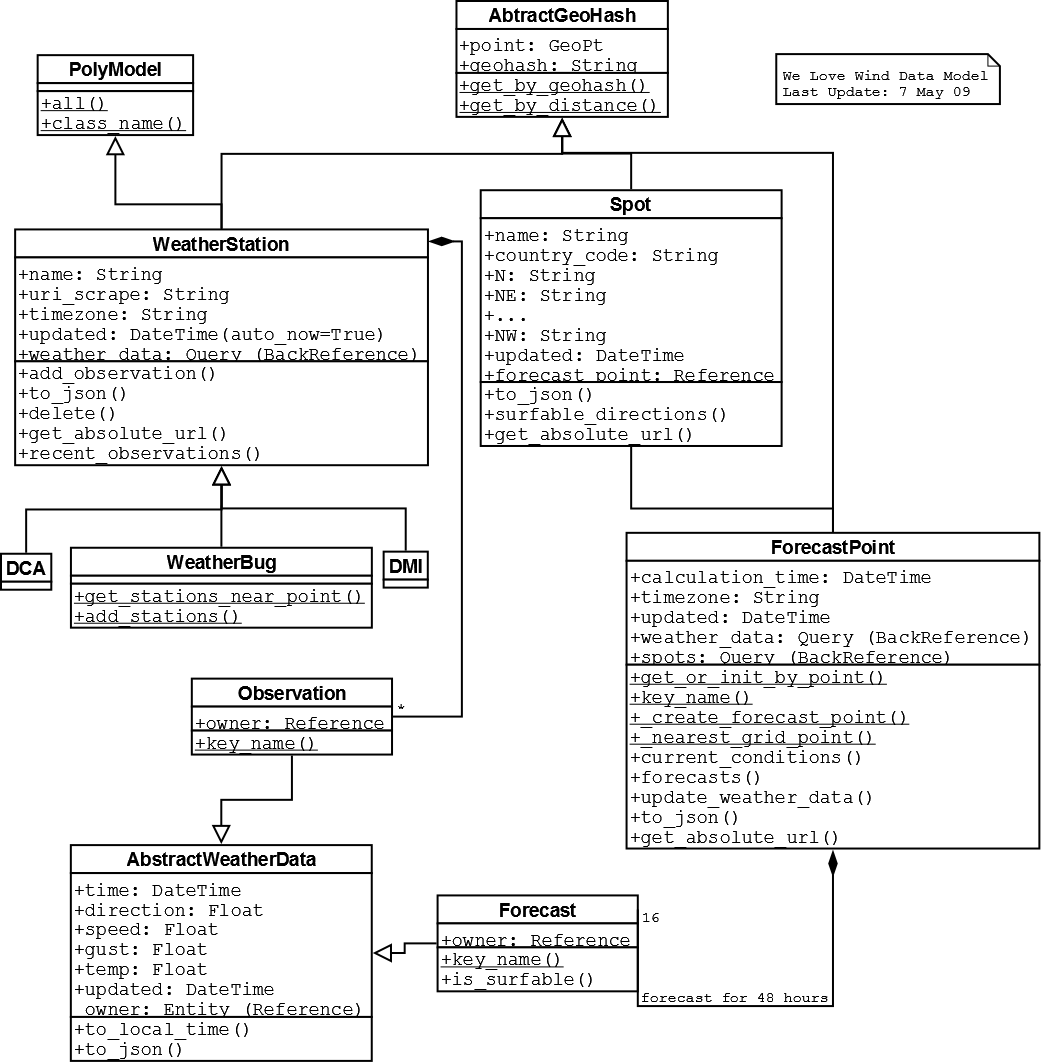
\includegraphics[width=\textwidth]{./Figures/DataModel}
  \caption{Data model (UML notation)}
  \label{fig:data_model}
\end{figure}

The models are not just defining the structure of data; the models contain all
the business logic of the application separating and encapsulating the data of
the application from the presentation of it.

Figure~\ref{fig:data_model} shows the data models of the application in a UML
static structure diagram. Arguments to methods is left out for brevity. Methods
underlined in the diagram are Python class methods. Since all data models inherit
from the \verb|db.Model| class it is omitted. The figure is a good mental model
to have in mind during the descriptions of the different model classes.

%%%%%%%
\subsection{AbstractGeoHash model}
Listing~\ref{lst:geohashmodel} shows the AbstractGeoHash model. The purpose of
the model is to provide geohash structure and logic for any model that inherits
from it; in that way all properties and methods relevant for geohashing is
factored out of the other models, i.e., spot, weather station, and forecast point.

\subsubsection*{Structure}
The model contains two properties: \verb|point| and \verb|geohash|. Point is the
 latitude and longitude for a place, and geohash is the geohash encoding of the
 latitude and longitude.

\subsubsection*{Logic}
The model contains logic that gets all points of the current class that have the
same geohash prefix as the given: manifested in \verb|get_near_geohash|. GQL
lacks the option to search for patterns in strings (\verb|LIKE| in SQL), instead
two inequality filter are applied to match the geohash prefix pattern; the last
filter sets the upper boundary of the range of results to return since the prefix
is concatenated with the largest possible unicode character: the replacement
character which is encoded as
\verb|u"\ufffd"|.\footnote{\url{http://en.wikipedia.org/wiki/Replacement_character}}

In addition, the model includes logic which retrieves all points within a
threshold distance of a given point: manifested in \verb|get_near_point|.  It
applies the geohash neighbors technique to get neighbors. The method uses
\verb|get_near_geohash| to get all points in the geohash areas; afterward pruning
the list to points within the threshold. Currently, the method assumes that the
radius (distance) from the center point is within the geohash neighbors.

Instances of the \verb|GeoHash| model automatically get a geohash value, since
the \verb|put| method is overwritten, and before saving the instance to the
datastore the geohash value is calculated and set. 

\begin{lstlisting}[caption=GeoHash model, label=lst:geohashmodel]
class AbstractGeoHash(db.Model):
    
    point = db.GeoPtProperty(required=True)
    geohash = db.StringProperty()
    
    @classmethod
    def get_near_geohash(cls, ghash_prefix, geohash_offset):
        ghash_prefix = ghash_prefix.lower()
        query = db.Query(cls)
        query.filter('geohash >=', geohash_offset)
        query.filter('geohash <', ghash_prefix + u"\ufffd")
        return query
    
    @classmethod
    def get_near_point(cls, point, distance, geohash_prefix_length = 3):
        entities = []
        center = geohash.encode(point.lat, point.lon)[:geohash_prefix_length]
        ghashes = geohashneighbors.neighbors(center)
        ghashes.append(center)
        
        for h in ghashes:
            query = cls.get_near_geohash(h,h)
            for entity in query:
                entities.append(entity)

        def prune(list):
            '''Prune a sorted list by distance'''
            for i, point in enumerate(list):
                if point.distance > distance:
                    return list[:i]
            return list
        
        return prune(geo.sort_by_distance(point, entities))
            
            
    def put(self):
        self.geohash = geohash.encode(self.point.lat, self.point.lon)
        return super(AbstractGeoHash, self).put()
\end{lstlisting}

%%%%%
\subsection{Spot model}
Listing~\ref{lst:spot_model} shows the Spot model. 

\subsubsection*{Structure}
The spot model inherits from the \verb|AbstractGeoHash| model: getting both a
\verb|point| and a \verb|geohash| property. Every spot has a \verb|name|, and, as
discussed in the resource section, every spot belongs to the nearest
\verb|forecast_point|. The many-to-one relationship between spots and forecast
points is implemented with the reference property.  The wind diagram is defined
as string attributes that must have one of four values: NO, MAYBE, YES, or
UNDEFINED.

The model has an updated property which is a pervasive property in
the data models. The property is automatically updated to the current datetime
each time the model is saved. This is useful for tracking the times of last
modification of entities, e.g., essential for implementing HTTP caching.

\subsubsection*{Logic}
There are two pervasive methods located on concrete models: \verb|to_json| and
\\\verb|get_absolute_url|. The \verb|to_json| method returns a simple Python object
representation of the instance ready for JSON serialization. The method will
prove its worth when we construct resource representations in the controllers in
Section~\ref{sec:controllers}.

The \verb|get_absolute_url| method return the URI for the concrete model; the
advantage is that changing the URI can now be done by just changing that method,
instead of refactoring all views.

As in the case with the \verb|AbtractGeoHash| model, the \verb|put| method is
overwritten to wire in some data. After saving a spot it is always associated
with the nearest forecast point and, in addition, the geohash value is wired into
the spot.

\begin{lstlisting}[caption=Spot model, label=lst:spot_model]
class Spot(AbstractGeoHash):
    WIND_DIAGRAM_CHOICES = ('NO','MAYBE', 'YES', 'UNDEFINED') 
    
    name = db.StringProperty(required=True)
    updated = db.DateTimeProperty(auto_now=True)
    country_code = db.StringProperty(required=True)
    forecast_point = db.ReferenceProperty(ForecastPoint, collection_name='spots')
    
    # wind diagram
    N  = db.StringProperty(default='UNDEFINED', choices=WIND_DIAGRAM_CHOICES)
    (...)
    NW = db.StringProperty(default='UNDEFINED', choices=WIND_DIAGRAM_CHOICES)
    
    def put(self):
        self.forecast_point = ForecastPoint.get_or_init_by_point(self.point)
        return super(Spot, self).put()
    
    @classmethod
    def key_name(self, country_code, name):
        return '/spots/%s/%s/' % (country_code, name)
    
    def to_json(self):
        return {
            'name':self.name,
            'country_code':self.country_code,
            'lat': self.point.lat,
            'lon': self.point.lon,
            'wind_diagram': self.surfable_directions(),
            'uri': self.get_absolute_url(),
            'forecast_point': self.forecast_point.get_absolute_url()
        }
        
    def get_absolute_url(self):
        return self.key().name()
(...)
\end{lstlisting}


\subsection{AbstractWeatherData Model}\label{sec:abstractweatherdatamodel}
The \verb|AbstractWeatherData| model, shown in
Listing~\ref{lst:abstract_weather_data_model} is a common supermodel for
forecasts and observations. Forecasts and observations have similar structure
except for the fact that forecasts belong to a forecast point and observations
belong to a weather station.

\subsubsection*{Structure}
The WeatherData model contains all the relevant weather data types mentioned
before: \verb|speed|, \verb|gust|, \verb|temp|, \verb|direction|, and a
\verb|time| of when the weather data applies. The model is abstract delegating
the references to its subclasses: Observation and Forecast. 

\begin{lstlisting}[caption=AbstractWeatherData model,label=lst:abstract_weather_data_model]
 class AbstractWeatherData(db.Model):
    '''Abtract weather data model.
    
    Attributes:
        is_new: indicates if this model is just created. Used by update_or_insert()
    
    Properties:
        updated: time of update on this server
        time: the observation / forecast time
    '''
    updated = db.DateTimeProperty(auto_now=True)
    direction = db.FloatProperty()
    speed = db.FloatProperty()
    temp = db.FloatProperty()
    gust = db.FloatProperty()
    time = db.DateTimeProperty(required=True)
    #abstract owner = db.ReferenceProperty()
    
    def __init__(self, is_new = False, **kwds):
        self.is_new = is_new
        super(AbstractWeatherData, self).__init__(**kwds)
        
    @classmethod
    def update_or_insert(cls, **kwds):
        key_name = cls.key_name(**kwds)
        entity = super(AbstractWeatherData, cls).get_or_insert(key_name, is_new=True, **kwds)
        if not entity.is_new:
            for prop in kwds.keys():
                setattr(entity, prop, kwds[prop])
            entity.put()
        return entity
(...)
\end{lstlisting}

\subsubsection*{Logic}
In an environment where weather data is continuously added eventually the
datastore will fill up. The datastore limit demands that some house keeping is
done. GAE cron jobs are limited in their number and duration time
\citep{Google:cron} and are not a scalable solution. An alternative to cleaning
up the datastore with cron jobs is needed.

An idea is continuously maintaining the datastore as new data is fed into it by
throwing out the oldest data. If we let, e.g., the last 24 hours of observations
and only the forecasts from the last calculation be in the datastore the amount
of weather data is pruned.

We let the weather data have a unique property, pertaining to the owner (weather
station or forecast point) and the time, e.g., a time delta such as total time of
day in minutes. When these properties are unique, inserting new data with the
same time delta and owner updates the existing entity. Implementation of unique
properties in the context of forecasts was presented in
Section~\vref{sec:unique_props}.

If the incoming data is consistently produced at certain times of the day the
technique is \textit{\gls{gls:fifo}} with a buffer size proportional to the
number of atomic units in the maximum time delta. In the case of observations the
buffer size is one day and the unit size is in minutes; that gives a maximum of
60 minutes * 24 hours = 1440 entities in the datastore per weather station. In
the case of forecasts the buffer size is 48 hours, however, since the time of
forecasts are always in hours the unit size is in hours; that gives a maximum of
48 entites per forecast point.

%% There are a total of 90 wind icons in the application. A certain wind icon is valid
%% for a certain speed interval and certain direction
%% interval. \verb|_direction_interval| maps from a direction number to a direction
%% string, which is the first part of the icon name. \verb|_speed_interval|
%% maps from the speed to a string indicating the interval the speed belongs to, the
%% last part of the icon name. \verb|wind_icon|, using that two methods, creates the
%% path to the icon representing the weather data.

\subsection{WeatherStation Model}\label{sec:ws_model}
Listing~\ref{lst:weather_station_model} shows the WeatherStation model. 

\subsubsection*{Structure}
The model inherits from the \verb|PolyModel| and the \verb|AbstractGeohash|. The
\verb|PolyModel| class provides a programmatic implementation of object
inheritance in the datastore similar to using NULL values to combine hierarchy
relations in relational databases \citep[sec.4.6]{db:Garcia-Molina:08}. The
advantage is that a query on the superclass includes all the entities from the
subclasses, and a query on the subclass only includes entities from the subclass.
The model has a list of observations. This is not visible in the model since it
is the reference property in the observation model that defines the one-to-many
relationship between weather stations and observations.

\subsubsection*{Logic}
The model is the owner of weather observations. As mentioned we overwrite
those observations on a circular basis. The model includes a method,\\
\verb|update_or_insert_observation|, that takes an observation resource in
deserialized JSON format and either inserts the observation or overwrites an
existing based on the unique properties of the observation model.


\begin{lstlisting}[label=lst:weather_station_model,caption=WeatherStation model]
class WeatherStation(polymodel.PolyModel, AbstractGeoHash):
 """Super model class for weather stations.
    Properties:
        name: name of weather station.
        updated: time of last update.
        country_code: country code of country where weather station is.
        weather_data: associated weather data
        uri_extern: URI to weather station
        uri_scrape: URI to scrape
    """
    name = db.StringProperty(required=True)
    uri_scrape = db.StringProperty()
    country_code = db.StringProperty(required=True)
    timezone = db.StringProperty(required=True)
    updated = db.DateTimeProperty(auto_now=True)
    # weather_data ref. from observation
    
    @classmethod
    def key_name(cls, country_code, slug):
        return '/weather_stations/%s/%s/' % (country_code, slug)
    
    def update_or_insert_observation(self, json):
        '''Update or insert observation to this station's weather data.
        
        Args:
            json: deserialized json weather data
                time (required): isoformat time 
                speed (not required):
                gust (not required):
                direction (not required):
        Returns:
            the updated/new observation.
        '''
        dt = wlwtime.ISO2dt(json['time'])
        
        entity = Observation.update_or_insert(
            owner=self,
            time=dt,
            speed = json.get('speed', None),
            gust = json.get('gust', None),
            temp = json.get('temp', None),
            direction = json.get('direction', None)
        )
        return entity
    
    def to_json(self):
        return {
            'name': escape(self.name),
            'type': self.class_name(),
            'timezone': self.timezone,
            'lat': self.point.lat,
            'lng': self.point.lon,
            'uri_scrape': self.uri_scrape,
            'uri': self.get_absolute_url(),
            'uri_observations': '%sobservations/' % self.get_absolute_url()
        }
(...)
\end{lstlisting}

\subsection{ForecastPoint model}
Listing~\ref{lst:forecast_model} shows the \verb|ForecastPoint| model. 

\subsubsection*{Structure}
The forecast point resource, presented in Section~\ref{sec:res:forecast_points},
contains a number of forecasts for a specific forecast point. This is a
many-to-one relationship between the forecast point and the forecasts of the
point. The relationship is manifested by the reference property from the
\verb|Forecast| Model to the \verb|ForecastPoint| model.

A forecast point is uniquely identified by its latitude and longitude; we
incorporate the point information into the key name of every instance hereby
ensuring that no two instances can have the same latitude and longitude.

\subsubsection*{Logic}
It is useful if the application does not load the datastore with all forecast
points in the world, since the forecast points are continuously updated. Surf
spots will for sure not use the majority of the forecast points. Therefore the
forecast points are added just-in-time when a spot is created. The
\verb|get_or_init_by_point| is the method that contains the logic to add forecast
points just-in-time. The method takes the following sequence of steps:
\begin{enumerate}
  \item Since forecast points are located in a granularity of 0.5� degrees, it
calculates the nearest grid point in the gfs grid.
  \item Checks for an existing point and returns the point if so; else, if the
  point does not exist, the point is created. Creating the point includes
  retrieving the timezone of the point from \url{geonames.org} and retrieving
  forecasts from the author's weather service at DAIMI, presented in
  Chapter~\ref{chap:ws_daimi}.
\end{enumerate}

The process includes calls to two external resources which obviously includes a
significant latency. However, it is only the first time the application access a
particular point that the latency is present.

The \verb|update_weather_data| method takes a weather forecast representation,
shown in Listing \vref{lst:forecast}, and updates the forecast point with all the
forecast in the representation. It iterates through all the forecasts using the
\verb|update_or_insert| method everytime putting the updated forecast to the
datastore.

\begin{lstlisting}[caption=Forecast model,label=lst:forecast_model]
class ForecastPoint(AbstractGeoHash):
    timezone = db.StringProperty(required=True)
    calculation_time = db.DateTimeProperty()
    # weather_data ref.

    @classmethod
    def get_or_init_by_point(cls, point):
        '''Get the forecast point nearest the given lat, lon.
        
        Returns:
            the (new saved) forecast point.
        '''
        nearest = ForecastPoint._nearest_grid_point(point)
        
        # Get the forecast point for the given point.
        forecast_point = ForecastPoint.get_by_key_name(ForecastPoint.key_name(nearest.lat, nearest.lon))
        
        if forecast_point:
            return forecast_point
        else:
            return ForecastPoint._create_forecast_point(nearest)
    
    @classmethod
    def _create_forecast_point(cls, nearest):
        '''Create new forecast point.
        
        Args:
            nearest: nearest grid point (GeoPt)
        Returns:
            forecast point with forecasts added.
        ''' 
        try:
            forecasts = daimiweather.get_forecasts(nearest)
        except Exception:
            forecasts = []
            calc_time = datetime.datetime.utcnow()
            tzinfo = {'timezoneId':'UTC'}
            
        if forecasts:
            # timezone from geonames.org
            try:
                response = geoinfo.geonames_timezone(nearest)
                tzinfo = simplejson.loads(response.content)
                calc_time = wlwtime.ISO2dt(forecasts['calculation_time'])
            except WSException:
                tzinfo = {'timezoneId':'UTC'}
                calc_time = datetime.datetime.utcnow()
                
        forecast_point = ForecastPoint(
            key_name=ForecastPoint.key_name(nearest.lat, nearest.lon),
            calculation_time=calc_time, 
            point=nearest,
            timezone=tzinfo['timezoneId'])
        
        forecast_point.put()
        
        # add all forecasts
        if forecasts:
            for f in forecasts['weather_data']:
                Forecast.update_or_insert(
                    calculation_time=calc_time,
                    owner = forecast_point,
                    speed = f.get('speed', None),
                    temp = f.get('temp', None),
                    direction = f.get('direction', None),
                    time = wlwtime.ISO2dt(f.get('time')))
        
        return forecast_point 
                 
    def forecasts(self, limit=19):
        '''        
        Returns:
            the weather data valid now and in the future.
        '''
        now = datetime.datetime.utcnow()
        now -= datetime.timedelta(hours=3)
        return self.weather_data.filter('time >=', now).order('time').fetch(limit)
    
    def update_weather_data(self, post_data):
        '''Update this point's weather data.
        
        Args:
            post_data: dictionary of key / value pairs from POST.
                calculation_time: iso time string of calculation time.
                weather_data: the weather data to update with.
        '''
        self.calculation_time = wlwtime.ISO2dt(post_data['calculation_time'])
        
        for data in post_data['weather_data']:
            Forecast.update_or_insert(
                calculation_time=self.calculation_time, 
                owner=self, 
                speed = data.get('speed', None),
                temp = data.get('temp', None),
                direction = data.get('direction', None),
                time = wlwtime.ISO2dt(data.get('time')))
        self.put()
(...)
\end{lstlisting}


\section{Implementation of Controllers}\label{sec:controllers}
The resources of the Web Service are composed of the data models in our
GAE/Django application. The resources are not equal to the data models, however,
the resources are equal to the URIs exposed, which are all backed by a controller. We
summarized the resources in the resource views in Chapter~\ref{chap:resources};
we now realize them in Django.

URIs are modeled in Django without any restrictions by the framework. URIs are
mapped to controllers by regular expressions that matches on the request's
URI. The regular expressions together with the controllers are registered in the
Python module \verb|urls.py| shown in Listing~\ref{lst:uris.py}. The code defines
patterns that map from an URI to a controller.

The regular expression functionality used is somewhat esoteric; therefore, we
give a short description of it. \verb|\w| is a predefined set of characters,
namely the character class consisting of all alphanumeric characters.  A
character class is defined by the content inside the metacharacters \verb|[| and
\verb|]|. In the case of \verb|[\w-]| the character class is the set of
alphanumeric characters and a dash. \verb|(?P<any_name>...)| defines a named
group; the matched content of these can later be referred to by name.

\begin{lstlisting}[caption=urls.py, label=lst:uris.py]
urlpatterns = patterns('',
  (r'^api/weather_stations/(?P<country_code>\w+)/(?P<id>[\w-]+)/$', WeatherStationsController()),
  (r'^api/weather_stations/(?P<country_code>\w+)/$', WeatherStationsController()),
  (r'^api/weather_stations/$', WeatherStationsController()),
    
  # weather observations
  (r'^api/weather_stations/(?P<country_code>\w+)/(?P<ws_id>[\w-]+)/observations/$', weather_observations.ObservationsController()),
)

# forecasts
urlpatterns += patterns('',
  (r'^api/forecast_points/info/$', forecasts.info),
  (r'^api/forecast_points/(?P<id>.+)/$', forecasts.ForecastPointsController()),
  (r'^api/forecast_points/$', forecasts.ForecastPointsController()),
)

# spots
urlpatterns += patterns('',    
  (r'^api/spots/(?P<country_code>\w+)/(?P<id>[\w-]+)/$', spots.SpotsController()),
  (r'^api/spots/(?P<country_code>\w+)/$', spots.SpotsController()),
  (r'^api/spots/$', spots.SpotsController()),
)
\end{lstlisting}

The patterns are quite powerful: they capture all requests to individual and list
resources of spots, forecast points, weather stations, and weather observations,
and route them to a corresponding controller. The controllers are usually Python
functions, but we take advantage of the fact that the controller can be any
callable object. The reason is that we want separation of concerns with regard to
the HTTP method of the requests. Thus, instead of handling the different HTTP
method types in each controller function we define a common REST controller class
that route to a Python method corresponding to the HTTP method.

\subsection{REST controller}
Table~\ref{tab:resourceinterface} shows the methods of the REST controller class
and how the methods correspond to URIs and HTTP method. As mentioned in
Section~\ref{sec:ws_uniform_interface} the POST method can be used to support PUT
and DELETE from (X)HTML by overloading it.  The approach is supported by the REST
controller. The URI pattern in the table is common in Web development; having an
items resource, and a resource for the specific items.

Listing~\ref{lst:rest_controller} shows the REST controller. Each of the Python
methods \verb|get|,\verb|index|, \verb|post|, \verb|put|, and \verb|delete|
correspond to a resource action that must be overridden in the subclass
inheriting from the REST controller in order to support the action. Invoking a
method that is not overridden in the subclass causes an HTTP
\verb|405 Method Not Allowed|. A 405 must include the allowed methods
\cite[sec.10.4]{w3:HTTP}, therefore the allowed methods are extracted and
returned.

The controller must distinguish between resources and subordinate resources. The
subordinate case is distinguished from the other by having the key name in its
URI. This is used in the method \verb|_get_permitted_methods| and
\verb|_handle_get| and \verb|_handle_post| to distinguish the two cases.

The Django patterns take any callable object as input, e.g., a function or a
method. An instance is callable if it contains the \verb|__call__| method. This
is used in the REST controller: upon start up of the Django application an
instance of the \verb|RESTController| is created. A pattern match triggers a call
to the corresponding instance, hereby executing the \verb|__call__| method.

\begin{table}
\centering
\begin{tabularx}{\textwidth}{l l l}
\toprule
Resource action & URI & HTTP Method\\\midrule

\verb|delete|, subordinate resource
& \verb|/{res.}/{res. id}/| & DELETE\\

\verb|index|, of all subordinate resources  
& \verb|/{res.}/| & GET\\

\verb|post|, new subordinate resource      
& \verb|/{res.}/| & POST\\

\verb|put|, existing subordinate resource         
& \verb|/{res.}/{res. id}/| & PUT\\

\verb|show|, subordinate resource
& \verb|/{res.}/{res. id}/| & GET\\\bottomrule
\end{tabularx}
\caption{REST controller-action to URI and HTTP method mapping}
\label{tab:resourceinterface}
\end{table}

The first argument given by Django to the callable object is always an
\verb|HttpRequest|, additional values captured by the regular expression are
parsed as subsequent arguments. Therefore the \verb|__call__| method takes a
request and an arbitrary number of keyword arguments: the values
from the named groups in the regular expressions. The method saves relevant
values in the instance and does a reflective look-up based on the request's HTTP
method. The method look-up resolves to one of four methods:
\verb|_handle_delete|, \verb|_handle_get|, \verb|_handle_post|, or
\verb|_handle_put|. \verb|_handle_post| is interesting since it handles
overloaded \verb|POST|. If \verb|POST| is overloaded yet another reflective
look-up is made according to the value of the \verb|_method| query parameter.

The controller supports two representation types from the client: the usual
uri-encoding type, and the \verb|application/json| type. All browsers upon
submitting forms with \verb|POST| convert the form data to uri-encoding, and put
the data in the message body of a POST request.

In Django, on the first access to the \verb|POST| or \verb|GET| data of a
\verb|HttpRequest|, Django parses the request data into a query dictionary that
expects uri-encoded data. This is useful if data is indeed in that format. This
is not the case when JSON is used as representation format. Parsing of the data
is bypassed by accessing the \verb|raw_post_data| member of the request, used
 in the \verb|_load_post_data| that parses data according to the
type of the content: JSON or uri-encoded.

\lstinputlisting[caption=REST controller,label=lst:rest_controller]{../implementation/wlw/wlw/controllers/rest_controller.py}

With the base controller in place we now turn to implementing the concrete
controllers of the resources; all inheriting from the REST controller.

\subsection{Spots controller}
The spots controller implements the spot resources from
Table~\vref{tab:spot_resources}. Clients create, read, and update spots reflected
in the controller that implements \verb|index|, \verb|put|, and \verb|post|.

\verb|index| serves all spots potentially filtered by country in a JSON
representation. Several query parameter filters can be applied:
\verb|geohash|, and \verb|geohash_offset|.

The JSON resource representation is created by first assembling a simple Python
object structure and then using simplejson\footnote{JSON encoder/decoder for Python}
to convert the structure to a JSON encoded string. By simple we mean that the
structure uses only simple Python constructs like dictionaries, lists, unicode,
etc. that have a corresponding construct in JSON; thus, allowing
serialization.\footnote{The documentation for simplejson includes all the allowed
constructs
\url{http://simplejson.googlecode.com/svn/tags/simplejson-2.0.9/docs/index.html}}

The representation of spots includes a maximum 100 spots. Paging of spots is
handled with the \verb|geohash_offset| query parameter. The application always
returns spots in ascending order sorted by geohash value. When more than 100
spots are present the representations point to the next geohash value in the
datastore; an example:
\begin{verbatim}
(...)
"next": "/api/spots/?geohash_offset=swgv3sxf003p"
(...)
\end{verbatim}
A request for that \verb|next| resource includes the 100 next spots with geohash
greater than or equal to \verb|geohash_offset|. This somewhat odd approach is the
only way to page geohash models. In-equality filters in queries are restricted to a
single property; in this case used on geohash; therefore, no other property can
act as the property for paging.

New spots are created with \verb|post|. The incoming representation is validated
with Django forms and saved if it is valid. A JSON representation is returned
both on success and failure caused by validation errors. The representation fits
the format of the jQuery forms plugin, which we use in Ajax frontend. 

\verb|put| is similar to \verb|post|, except that it demands existence of the
resource.

\begin{lstlisting}[caption=Spots controller,label=lst:spots_controller]
PAGE_SIZE = 100

class SpotsController(RestController):
    
    def index(self):
        geohash = self.request.GET.get('geohash')
        geohash_offset = self.request.GET.get('geohash_offset', '')
        
        if geohash:
            spots = Spot.get_near_geohash(geohash, geohash_offset)
        else:
            spots = db.Query(Spot).order('geohash').filter('geohash >=', geohash_offset)
        
        country_code = self.kwargs.get('country_code')
        if country_code:
            spots.filter('country_code =', country_code)
        
        # fetching one more to check for has_next
        entities = spots.fetch(PAGE_SIZE + 1)
        
        qs = None
        has_next_page = (len(entities) > PAGE_SIZE)
        
        if has_next_page:
            qs = self.request.GET.copy()
            qs['geohash_offset'] = entities[-1].geohash

        repr = {
            'next': '%s?%s' % (self.request.META['PATH_INFO'], qs.urlencode()) if has_next_page else '',
            'items': [s.to_json() for s in entities]
        }
        
        return http.HttpResponse(simplejson.dumps(repr), mimetype='application/json')

    def put(self, id):
        (...)            
        
    def post(self):
        form = SpotForm(self.request.POST)
        
        if not form.errors:
            spot = form.save()
            
            # add weather stations
            stations = WeatherBugWeatherStation.get_stations_near_point(spot.point)
            keys = WeatherBugWeatherStation.add_stations(stations) 
            
            result = {'type': 'success', 'message':'Spot %s created' % spot.name, 'spot': spot.to_json()}
            if len(keys) != 0:
                result['message'] += '. Added Weather stations: %s' % keys
            
            json = simplejson.dumps(result)
            response = http.HttpResponse(json, mimetype='application/json')
            response.status_code = 201 
            response['Location'] = spot.get_absolute_url()
            return response
        else:
            result = {'type': 'error', 'message': form.errors.as_ul()}
            return http.HttpResponse(simplejson.dumps(result), mimetype='application/json')    
\end{lstlisting}

An interesting thing with \verb|post| is that it adds weather stations from WB in
the area of the new spot to the application. Section~\vref{client:weatherbug}
presents how.

\subsection{Weather stations controller}
The weather station controller implements the resources in
Table~\vref{tab:ws_resources}. It merely serves JSON representations of the
weather station list resource, corresponding to the \verb|index| method.

The \verb|index| method differs from the corresponding method of the spots
controller only in adding filters on the type of weather station, and on the type
of the time format used in the representation; therefore, the code is omitted. 

\subsection{Observations controller}
We still need to realize the last resource from Table~\vref{tab:ws_resources}:
the observations resource. The key to realize the resources is the regular
expression in Listing~\vref{lst:uris.py}: the regular expression attach the
observations controller under weather stations URIs. This means that the
\verb|country_code| and the weather stations id (\verb|ws_id)| is available for
the observations controller. The two values are used to fetch the weather station
from which observations are fetched.

The resource expose \verb|GET| and \verb|POST| from the uniform interface
manifested in \verb|index| and \verb|post|, shown in
Listing~\ref{lst:observations_controller}. \verb|index| is similar to the
previous \verb|index| methods, however, it fetches the weather station as the
first thing in order to fetch the right observations. \verb|post| creates or
updates observations with the resource in the request. It uses the
\verb|update_or_insert_observation| of the weather station model which realizes
\gls{gls:fifo} for observations.

\begin{lstlisting}[caption=Observations controller,label=lst:observations_controller]
class ObservationsController(RestController):   
    def index(self):
        '''Get list of observations.
        
        Query Args:
            limit: the number of observations to fetch.
            time_format: (ietf|iso) format of times. Default is ISO format.
        Returns:
            latest observations.
        '''
        ws_key_name = WeatherStation.key_name(self.kwargs['country_code'], 
            self.kwargs['ws_id'])
        ws = dbutils.get_object_or_404(WeatherStation, key_name=ws_key_name)
        
        observations = ws.weather_data.order('-time')
        (...)

    def post(self):
        '''POST create or update 1 weather observation to this weather station.
        
        Args POST:
            json weather data: 
                time (required): isoformat time 
                speed (not required) 
                gust (not required)
                direction (not required)
        '''
        ws_key_name = WeatherStation.key_name(self.kwargs['country_code'], 
            self.kwargs['ws_id'])
        ws = dbutils.get_object_or_404(WeatherStation, key_name=ws_key_name)
        ws.update_or_insert_observation(self.post_data)
        return HttpResponse("Weather observation created")
\end{lstlisting}

\subsection{Forecast points controller}
The forecast point controller, shown in
Listing~\ref{lst:forecast_points_controller}, realizes the resources in
Table~\vref{tab:for_resources}. The only conceptually new method is \verb|show|,
which returns a JSON representation of concrete forecast points including its
forecasts. \verb|show| takes the following sequence of steps:
\begin{enumerate}
  \item extracts the latitude and longitude from the URI;
  \item finds the forecast point (or returns 404 if un-existing); and
  \item creates a JSON representation and returns it.
\end{enumerate}

\begin{lstlisting}[caption=Forecast points controller, label=lst:forecast_points_controller]
class ForecastPointsController(RestController):
    
    def index(self):
      (...)
    def put(self, id):
      (...)
    def show(self, id):
        '''Show concrete forecast point.
        Args:
            id: id of forecast point
        Args GET:
            time_format: (ietf|iso) iso is standard
        '''
        key_name = _extract_key_name(id)
        forecast_point = dbutils.get_object_or_404(ForecastPoint, key_name=key_name)
        time_converter = wlwtime.dt2IETF if self.request.GET.get('time_format') == 'ietf' else wlwtime.dt2ISO
        repr = simplejson.dumps(forecast_point.to_json(include_forecasts=True, time_converter=time_converter))
        return http.HttpResponse(repr, content_type='application/json')
    
def _extract_key_name(id):
    '''Extract the lat and lon given as 10.0,10.0
    and return the key_name of the forecast point id'ed by the point.
    
    Returns:
        lat,lon: the latitude and longitude.
    '''
    latlng = id.split(',')
    lat = latlng[0]
    lon = latlng[1]
    return ForecastPoint.key_name(lat,lon)

\end{lstlisting}

\section{Implementation of Views}
The functionality of the Web Service is separated into the three layers of
MVC. Creating the views of the application is, however, so simple that they are
incorporated into the controllers. The controllers assembled a simple Python
object, converted it to serialized JSON using simplejson, and returned that in
the HTTP response.

\section{Enhancing Performance}
The performance of the Web Service is essential; applying explicit HTTP caching
can significantly increase the performance. The We Love Wind Web Service take
advantage of HTTP caching in most resources. In the following, we focus on how
the \verb|index| method in the Spot controller is altered to support caching.

Updates of the spots resources are infrequent. The spots resources are valid in
caches until a user adds a new spot or modifies a spot, however, an inconsistent
cached copy is not a significant problem, it should just be brought up to date
relatively fast. The \verb|index| method of the spots controller explicitly set
the duration of caches to one day.

The application can avoid transferring data over the network even if the cache
is expired by using \verb|ETag|s. A natural \verb|ETag| for spots resources are
the last time of modification of spot entities for the current page. The
representation of the spots resource sent back to clients is always attached with
an \verb|ETag| of the last modification time. Additional requests includes the
\verb|ETag| which is validated by the controller and only upon \verb|ETag|
mismatch the representation is sent back. Upon match the representation is
unmodified and the controller sends back an HTTP 304 to the client which then
uses its cached representation. The altered \verb|index| method of the spots
controller is shown in Listing~\ref{lst:caching_spots_controller}. In Django HTTP
headers are set directly in the response object.

\begin{lstlisting}[caption=Caching spots controller, label=lst:caching_spots_controller]
class SpotsController(RestController):
    
    def index(self):
        geohash = self.request.GET.get('geohash')
        geohash_offset = self.request.GET.get('geohash_offset', geohash)
        
        if geohash:
            spots = Spot.get_near_geohash(geohash, geohash_offset)
        else:
            spots = db.Query(Spot).order('geohash').filter('geohash >=', geohash_offset)
        
        country_code = self.kwargs.get('country_code')
        if country_code:
            spots.filter('country_code =', country_code)
        
        entities = spots.fetch(PAGE_SIZE + 1)
        
        # very long ago, day 1
        last_modified = datetime.datetime.fromordinal(1)
        items = []
        for s in entities[:PAGE_SIZE]:
            items.append(s.to_json())
            if s.updated > last_modified:
                last_modified = s.updated
        
        if str(last_modified) == self.request.META.get("HTTP_IF_NONE_MATCH"):
            return http.HttpResponseNotModified()
         
        qs = None
        has_next_page = (len(entities) > PAGE_SIZE)
        
        if has_next_page:
            qs = self.request.GET.copy()
            qs['geohash_offset'] = entities[-1].geohash
        repr = {
            'next': '%s?%s' % (self.request.META['PATH_INFO'], qs.urlencode()) if has_next_page else '',
            'items': items
        }
        
        response = http.HttpResponse(simplejson.dumps(repr), mimetype='application/json')
        
        response['Cache-Control'] = 'public, max-age=86400'
        response['Etag'] = last_modified
        return response
\end{lstlisting}

The complexity is increased but the speedup is significant. Spots are instantly
loaded in browsers on additional requests within 24 hours. \verb|ETag| caching,
however, does not offer a significant speed up: the following is a small test
with cURL and time.\footnote{ cURL is a tool to, e.g., issue GET requests to a
specified URI. Headers are specified with \verb|-H| and included in the output
with \verb|-i|}

\begin{verbatim}
$ time curl -i "http://www.welovewind.com/api/spots/?1"
HTTP/1.1 200 OK
Etag: 2009-06-15 08:14:58.829396
Content-Type: application/json
Cache-Control: public, max-age=3600
Date: Wed, 24 Jun 2009 11:25:10 GMT
Server: Google Frontend
Transfer-Encoding: chunked
(...)

real    0m0.622s
user    0m0.003s
sys     0m0.001s
\end{verbatim}

\verb|ETag| caching is tested, by setting the \verb|If-None-Match| header field
to the value of the \verb|ETag|.

\begin{verbatim}
$ time curl -i -H "If-None-Match:2009-06-15 08:14:58.829396" \
> "http://www.welovewind.com/api/spots/?2"
HTTP/1.1 304 Not Modified
Content-Type: text/html; charset=utf-8
Date: Wed, 24 Jun 2009 11:25:19 GMT
Server: Google Frontend

real    0m0.555s
user    0m0.001s
sys     0m0.004s
\end{verbatim}
%
In the example, the server returns a HTTP 304 which means that the response has
an empty body. The duration of the requests, however, are almost equal. To
investigate the case we issued a series of tests, however, with the same
result. The average of both are within 620 -- 660 ms. We note that the test was
issued with a different URI each time, bypassing intermediate caches and forcing
both request to hit the server.

We conclude that \verb|ETag| caching is not worth the trouble in terms of
latency if the representations are small and if it is not essential to reduce the
used bandwidth.

\section{Summary}
In this chapter, we described the design and implementation of a RESTful Web
Service with Google App Engine/Django. The implementation was described in terms
of the MVC style. Finally, we presented an example of how HTTP caching is applied
in the Web Service to reduce latency. %




%% A conditional GET is a normal HTTP GET augmented
%% with either  one of the headers \verb|If-Modified-Since: {datetime}|, \verb|If-Match|
%% etc., known as \verb|if-*| \url{http://www.w3.org/1999/04/Editing/}. 


%% The caching support makes the controllers\footnote{Django calls controllers
%% views, but to stay in terminology we shall call them controllers} more
%% complex. The controllers must contain logic to decide if the content on the
%% server has changed, compared to the content at the client. Models, therefore,
%% must support queries for modification times, by continuously updating a datetime
%% property of last modification on the model.


%%  but the performance gain is significant. Upon a request, the
%% server returns a HTTP 304 not modified response, if the resource is not modified,
%% instead of the whole resource. 




%% HTTP 1.1 \url{http://www.w3.org/Protocols/rfc2616/rfc2616.html}

%% INDEXES
% It might take a few hours before they are build and ready.


\chapter{The DAIMI Forecast Web Service}\label{chap:ws_daimi}
In the last chapter we described the We Love Wind Web Service. That service
included external calls to another Web Service: The DAIMI Forecast Web Service, found
at
\begin{itemize}
  \item \url{http://daimi.welovewind.com/}
\end{itemize}
There are important requirements in the application that demands an additional
forecast Web Service:
\begin{itemize}
  \item it should be possible to get forecasts for arbitrary locations; and,
  \item after creating new spots, the forecasts of the nearest forecast point
  should be in place immediately. 
\end{itemize}
If the logic to get forecasts were placed on GAE, the requirements are
trivial. The application is based on binary forecasts from NOAA. The decoding
software is incompatible with GAE; the decoding of the binary forecast files
demands that the decoding logic is placed elsewhere. It is infeasible to
continuously update all forecast points -- ca. 260000 points -- therefore, the
forecasts of points are only updated when relevant for surf spots, and that
demands an extra service for forecasts. In essence, we are wrapping a modern Web
Service around the binary forecasts files from NOAA.

In this chapter we describe the implementation of a RESTful weather service with
Python/CGI.\footnote{The Web Service is located at the department of computer
science, Aarhus University; that left the author with two options for generating
the dynamic output: PHP or CGI. To keep things consistent we implement the
forecast service in a Python CGI script.} The focus of this chapter is on the
implementation of the Web Service; we postpone the description of retrieving and
converting weather data to the next part.

The resource of the service is already defined: it is the forecast points
resources described in Section~\vref{sec:res:forecast_points}. Therefore, we jump
directly to the implementation; again described in terms of the MVC style.

\section{Model}
The forecast weather service contains a single model: the forecast point
model. The purpose of the model is to encapsulate the access to the weather
forecasts located in files. 

\subsection*{Structure}
The model contains three properties: the latitude and longitude of the point, and
the forecasts of the point.

\subsection*{Logic}
The forecast point model is able to return a representation of itself in JSON
format. The main method in the model is a class method that retrieves the current
and all future forecast from the gfs files; since decoding forecasts from the
forecast files takes about 0.5 seconds the method takes a maximum argument that
reduces the number of returned forecasts.

\section{Controller}
 The controller is implemented as a Python/CGI script. CGI is a standard that
connects a server with any programming language. Responses are crafted by
printing the headers of the HTTP response which must include a
\verb|content-type| header, the header is ended with an empty line and after that
the program prints the body of the response.

Listing~\ref{lst:cgi_forecast_point_controller} shows the
controller. \verb|handle_request| is the entry method; it starts by extracting
the parameters of the request. The values of those parameters are later given to
an external shell program as arguments; therefore, the parameters are sanitized
and parsed as floats avoiding security issues. If any error occur during this
process the response signals the error with a HTTP 400 Bad Request. Secondly, the
extracted parameters are given to the model which populates itself with forecast
data according to the arguments. Finally, if caching does not apply the forecast
point is printed in JSON format. 

\begin{lstlisting}[caption=Forecast point CGI controller, label=lst:cgi_forecast_point_controller]
def handle_request():
    try:
        params = extract_params()
        if not params:
            print_intro()
            return
        forecasts = ForecastPoints(**params)
        if etag_match(forecasts):
            not_modified_304()
            return
        print_forecasts(forecasts)
    except (ValueError, IndexError):
        print_intro(400)

def extract_params():
    input = os.environ.get('REDIRECT_QUERY_STRING')
    lat, lon, maximum = None, None, 3 # maximum 3 if not specified
    if input:
        input = input.strip('/').split(',')
        lat = float(input[0])
        lon = float(input[1])
        if lat < -90.0 or lat > 90.0 or lon < -180.0 or lon > 180.0:
            raise ValueError
        match = re.search(r'max=(\d+)', os.environ.get('REQUEST_URI'))
        if match:
            maximum = int(match.group(1))
        return {'lat':lat, 'lon':lon, 'maximum':maximum}
    else:
        return None

def print_intro(status=None):
    print 'Content-type: text/plain'
    if status:
        print 'Status: %s' % status
    print
    print 'Welcome to the DAIMI Weather Forecasts Service'
    print 'forecasts are accessed by ..forecasts/{lat},{lon}'
    print 'the number of returned forecast is specified by setting the max query parameter: ../?max=10'

def print_forecasts(forecasts):
    print 'Content-type: text/plain'
    print 'ETag: %s' % forecasts.last_modified()
    print
    print forecasts.to_json()

def not_modified_304():
    print 'Status: 304 Not Modified'
    print

def etag_match(forecasts):
    etag = os.environ.get('HTTP_IF_NONE_MATCH')
    if etag:
        if forecasts.last_modified() == etag:
            return True
    return False

handle_request()  
\end{lstlisting}

\section{Summary}
In this chapter, we described the implementation of a forecast Web Service. We
designed two Web Services since NOAA forecasts was incompatible with GAE. At the
time of implementation the GAE lacked support for cron jobs, offline processing,
and Java. All the necessary components are now in place\footnote{Offline
processing of tasks is still experimental on GAE.} making a future solution that
is more clean and effective possible. Java is needed since there are limited
options to decode GRIB2 files: the unidata Java decoder
tools\footnote{\url{http://www.unidata.ucar.edu/software/decoders/}},
\verb|wgrib2|, and
\verb|pygrib2|\footnote{\url{http://pygrib2.googlecode.com/}}. The latter two are
incompatible with GAE since they are based on \verb|C| modules.

This ends the description of the Web Services (or the server-side) of the We Love
Wind mashup. In the following chapters we turn to the clients of those Web
Services.


\part{The Clients}
%% A Web Service client is the consumer of a Web Service. This part of the
%% dissertation describes the design and implementation of clients that consume the
%% Web Services described in the last part.

%% There are two clients meant for user consumption: the main front-end ()of the
%% application manifested in an Ajax client and a supplementary front-end manifested
%% in a Django client. The former is apt for standard computer whereas the latter is
%% apt for mobiles.
\begin{savequote}[10pc]
\sffamily
``It is a capital mistake to theorize before one has data.''
\qauthor{Sherlock Holmes, Sir Arthur Conan Doyle (1859 -- 1930)}
\end{savequote}
\chapter{Weather data}\label{chap:forecasts}

\section{Getting weather data}\label{sec:getting_weather_data}
The resources incorporate weather data -- forecasts and observations -- from four
external resources: DCA, DMI, WB, and NOAA. The weather data must be up to data
when the user requests the information. None of the sources provide JSON(P) 
Web Services therefore we must either use the GAE as a proxy or save the data
locally and periodically update the content. 7 April 2009 Google announced
support for scheduling cron
jobs\footnote{\url{http://code.google.com/p/googleappengine/issues/detail?id=6}},
giving three options for keeping the data up to date: either update the data
\begin{enumerate}
  \item by an internal cron job at the GAE;
  \item on-demand upon user HTTP requests; or,
  \item by an external cron job.
\end{enumerate}
%%
\textit{Internal cron jobs:} The natural choice would be an internal cron job at
the GAE, making the GAE responsible for consuming weather data from the external
resources at regular intervals. The cron jobs at Google are limited to the same
constraints as usual HTTP requests, e.g., the request duration limit. In
addition, the number of jobs are limited to 20, and at minimum there must be one
minute between individual cron jobs \citep{Google:cron}. With hundreds of weather
stations a naive cron job times out, and the changes done in the transaction are
rolled back. Since it is possible to execute cron jobs every minute, a workaround
is to limit the number of processed weather stations. Every data retrieval lasts
about one second which means that about 20 resources can be processed per minute
under the request duration limit. Weather stations are updated ca. every 20
minutes, which yields only 400 stations that can be updated on a continuously
basis per cron jobs, and which makes this approach infeasible.  \\\\
\textit{On-demand:} By on-demand we mean weather data is updated just-in-time
when the user needs the weather data. Because of the request duration limit the
approach would include requests from JavaScript at the client side for every
resource of interest, and the controller would update the GAE version of the
weather data if it is stale. The approach, however, includes a significant
latency. Getting weather data must be a low latency operation making the approach
infeasible.\footnote{GAE is an emerging technology. A promising GAE offering
(announced 18 June 2009) is the Task Queue. The Task Queue process tasks
independently of the originating request. The only problem is getting the updated
information back to the user, and not just to the next user accessing the
page. Such a requirement is typically realized with Comet (or Ajax Push),
however, this is not supported on GAE. If (or when) it is supported the Task
Queue together with Comet is a solution for the update problem.}  \\\\
\textit{External cron jobs:} The last option is letting external cron jobs pull
weather data from all the weather resource and push the data to the GAE. The
external updaters are tightly coupled to the GAE in a point-to-point solution
with much redundant data transfer, however, it is the best of the worst at the
moment.

\section{Weather Observations}\label{chap:observations}
Unfortunately we have no Swiss Army Knife for the problem of pulling information
from the different sources. The resources are diverse and in different formats;
therefore, each case is handled on an individual basis. 

\subsection{Scraping DMI and DCA}
The only option to get weather data from DCA and DMI is by scraping their Web
pages for content. Web scraping is the process of programmatically retrieving
content from a Web page meant for human consumption. The data at DCA is
inaccessible as a Web Service, but DCA has agreed to let their pages be accessed
by our Web Scraper in order to retrieve the data.

DMI prohibits incorporation of their data in other sites. The author has several
times asked DMI for a collaboration, however, un-successful. We might be crossing
ethical boundaries, but, we have decided to Web scrape their site, just like
Google does.

Content in the case of DCA is located at sub-pages on a station and data type
basis (speed, direction, and temperature are located at different pages). Content
at DMI is located in sub-pages on a weather station basis. 

All resources are invalid HTML and will cause an XML parser to fail. This is a
case where Beautiful
Soup\footnote{\url{http://www.crummy.com/software/BeautifulSoup/}}, a Python
module to Web scrape Web pages, has a great force; to quote their Web page:
%
\begin{quote}
\footnotesize\itshape
You didn't write that awful page. You're just trying to get some data out of
it. Right now, you don't really care what HTML is supposed to look like.\\
\\
Neither does this parser.
\end{quote}
%
Scraping the latest speed, direction, temp, and time from DMI Aarhus, the code in
Listing~\ref{lst:dmiscraper} is all that is needed (after downloading the
BeautifulSoup module).

\begin{lstlisting}[caption=DMI Web scraper, label=lst:dmiscraper]
months = ['', 'januar', 'februar', 'marts', 'april', 'maj', 'juni', 'juli', 'august', 'septempber', 'oktober', 'november', 'december']

def _scrape(ws):
    page = urlopen(ws['uri_scrape']).read()
    soup = BeautifulSoup(page)

    # all text from page
    text = soup.findAll(text=True)

    # time
    contents = text[6].split()
    day = int(contents[2].strip('.'))
    month = int(months.index(contents[3])) # januar -> 1
    year = int(contents[4])
    hour = int(contents[5].split(':')[0])
    minute = int(contents[5].split(':')[1])
    dt = datetime(year, month, day, hour, minute)
    iso_time_utc = convert_local_time_to_utc(dt.timetuple())

    # wind
    contents = text[7].split()
    direction = float(contents[1])
    speed = float(contents[3])

    # temp
    contents = text[8].split()
    temp = float(contents[1])

    return {'time':iso_time_utc, 'direction':direction, 'temp':temp, 'speed':speed}

def convert_local_time_to_utc(time_tuple):
    secs = time.mktime(time_tuple)
    utc = time.gmtime(secs)
    iso = time.strftime("%Y-%m-%dT%H:%M:%S", utc)
    return iso

if __name__ == '__main__':
    print _scrape({'uri_scrape':'http://servlet.dmi.dk/bv/servlet/bv?stat=6074'})
\end{lstlisting}
%
In the example we use the Python library \verb|urllib2| to fetch the page. This
is given as an argument to BeatifulSoup when it is instantiated. The
\verb|BeautifulSoup| class has many methods that assist in extracting relevant
data from the page; we use the \verb|findAll| method to find all elements, and
extract content from that list.

Scraping DCA's site is similar except that it needs tailoring for the specific
layout of that site. 

The Web scraper is fragile to modifications in the user interface, e.g.,
modification to the placement of the different data, but we have no other option
to retrieve the data.

\subsection{Scraping WB}\label{client:weatherbug}
In contrast to the ill-formed data from DCA the data from WB is in XML formats,
and therefore more apt for computer consumption. Listing~\ref{lst:weatherbug_rss}
shows an example of a WB XML document. The documents are subject to a single
operation: extraction of node content and node attribute values.

From an abstract viewpoint, there are two types of XML parsers: tree-based
parsers and event-based parsers. Tree-based parsers read in the whole XML
document at once and create an internal data structure, while event-based parsers
consider XML documents as a stream of events serially generating events while
parsing the document. In the previous section, we used a tree-based parser,
BeautifulSoup. The advantages of event-based frameworks over tree-based are that
they are fast and efficient since they avoid building a tree data structure;
the advantage, however, is at the expense of simplicity in the programming model.

XML parsing of WB data merely has the purpose of extracting content of specific
nodes: the application does not call for any transformations, and not for
processing dependent on former seen nodes, and not for fixing invalid XML;
therefore, we choose the event-based parser, SAX.\footnote{The Python standard
library contains both types of XML parsers: tree-based, manifested in the
Document Object Model\footnote{\url{http://docs.python.org/library/xml.dom.html}}
(DOM), and event-based, manifested in the Simple API for
XML\footnote{\url{http://docs.python.org/library/xml.sax.html}} (SAX).}

\begin{lstlisting}[caption=WeatherBug Weather RSS feed for weather station Tirstrup Airport,label=lst:weatherbug_rss]
(...)
  <aws:station requestedID="EKAH" id="EKAH" 
    name="Tirstrup Airport" 
    city="Tirstrup"  state="Denmark" 
    citycode="60090" country="Denmark" 
    latitude="56.2999992370605" 
    longitude="10.6166667938232" />
  <aws:current-condition 
    icon="http://deskwx.weatherbug.com/images/Forecast/icons/cond024.gif">
    Mostly Cloudy
  </aws:current-condition>
  <aws:temp units="&amp;deg;C">9.0</aws:temp>
  <aws:rain-today units="mm">0.00</aws:rain-today>
  <aws:wind-speed units="km/h">22</aws:wind-speed>
  <aws:wind-direction>ESE</aws:wind-direction>
  <aws:gust-speed units="km/h">21</aws:gust-speed>
  <aws:gust-direction>ESE</aws:gust-direction>
</aws:weather>
(...)
<pubDate>Wed, 15 Apr 2009 13:50:00 GMT</pubDate>
(...)
\end{lstlisting}

%% http://api.wxbug.net/getStationsXML.aspx?ACode=A5580954882&lat=56.15&long=10.21

Parsing with Python SAX is done by inheriting from the class
\verb|ContentHandler| and overwriting relevant methods. The methods correspond to
events generated when SAX parses the document.

A generic content handler that extract content must overwrite three methods in
the \verb|ContentHandler|: \verb|startElement|, \verb|endElement|, and
\verb|characters|. During parsing the \verb|startElement| method is called for
every XML start tag, the \verb|endElement| method is called for every XML end
tag, and the \verb|characters| method is called for each chunk of character
data.\footnote{For more info see \url{http://docs.python.org/library/xml.sax.handler.html}}

Listing~\ref{lst:sax_xmlparser} shows the code for the XML parser. The parser is
instantiated with a list of the type of XML elements from which to retrieve the
content. The parser keeps track of when it is inside relevant nodes with the
\verb|in_element| variable. The relevant node content is put in a dictionary of
XML-element keys and node content values.

% XML SAX Parser 
\lstinputlisting[caption=SAX XML parser,label=lst:sax_xmlparser]{../implementation/wlw/wlw/helpers/xmlparser.py}

Extracting the content of the RSS feed is now just a matter of picking the
elements to retrieve the node content from, and parsing the XML string with the
content handler, the code is shown in Listing~\ref{lst:weatherbug_scrape}.

\begin{lstlisting}[caption=Extracting XML content from WB station RSS feed,label=lst:weatherbug_scrape]
XML_ELEMENTS = ['aws:temp', 'aws:wind-speed', 'aws:wind-direction','aws:gust-speed', 'aws:gust-direction', 'pubDate']

def _scrape(ws):
    response = urllib2.urlopen(ws['uri_scrape']).read()
    values = {}
    parseString(response, XMLParser(values, XML_ELEMENTS))

    time = convert_local_time_to_utc(parse_wb_time(values['pubDate']))
    temp = parse_float(values.get('aws:temp'))
    gust = parse_float(values.get('aws:gust-speed'))
    direction = values.get('aws:wind-direction')
    speed = parse_float(values.get('aws:wind-speed'))

    if speed:
        speed = speed / 3.6 # from km/h to m/s

    if gust:
        gust = gust / 3.6

    if direction:
        direction = convert_direction(direction)

    return {'time':time, 'direction':direction, 'temp':temp, 'speed':speed, 'gust':gust}

    (...)

if __name__ == '__main__':
    print _scrape({'uri_scrape':'http://api.wxbug.net/getLiveCompactWeatherRSS.aspx?ACode=A5580954882&stationid=ETGG&unittype=1'})
\end{lstlisting}

\subsection{Integrating with the Web Service}
Web scraping the three types of weather stations is a similar process: 
\begin{enumerate}
  \item fetch all weather stations of a certain type from the Web Service; and
  for all weather stations,
  \item scrape it and post the new data to the Web Service.
\end{enumerate}
The only difference between the weather station types are in the concrete
scraping code. Therefore, we apply the template method pattern \citep{Gamma:1995}
and create a general scraper skeleton, deferring the concrete scraping code to
its subclasses.

\verb|update_weather_data| is the template method, shown in
Listing~\ref{lst:scraper}, that implements the process described above.
\verb|_scrape| is the deferred method, it uses the \verb|scrape_uri| from the
fetched representation and returns the scraped data as a simple Python object
compatible with the observation representation format
(see~\vref{lst:obs_res}). \verb|_update_server| converts the object to JSON, sets
the content type (used by the controller in the Web Service), and post the
representation to the server. \verb|_scrape| continues recursively if the
paginator contains more pages. The individual \verb|_scrape| methods were
presented in the last section and fit directly into the skeleton when they are
put in a class that inherits from \verb|Scraper|.

\begin{lstlisting}[caption=Common Web scraper,label=lst:scraper]
URI_BASE = 'http://www.welovewind.com'
URI_WEATHER_STATIONS = 'http://www.welovewind.com/api/weather_stations/'
class Scraper:

    def __init__(self, type):
        '''Craete instance of scraper
        Args:
          type: weather station type ('dmi'|'wb'|'dca')
        '''
        self.type = type

    def update(self):
        self.update_weather_data(URI_WEATHER_STATIONS + '?type=%s' % self.type)

    def update_weather_data(self, uri):
        '''Template method'''
        wss = self._fetch_weather_stations(uri)
        for ws in wss['items']:
            data = self._scrape(ws)

            # update server
            uri = '%s%s' % (URI_BASE, ws['uri_observations'])
            self._update_server(uri, data)
        if wss['next']:
            self.update_weather_data('%s%s' % (URI_BASE,wss['next']))

    def _fetch_weather_stations(self, uri):
        response = urllib2.urlopen(uri)
        return simplejson.load(response)


    def _scrape(self, ws):
        raise Exception('Abstract Method')

    def _update_server(self, uri, data):
        try:
            json = simplejson.dumps(data)
            # putting in the values will cause the request to be a POST
            request = urllib2.Request(uri, json, {'Content-Type': 'application/json'})
            response = urllib2.urlopen(request).read()
        except urllib2.HTTPError, e:
            logging.error('trying to post data: %s' % data)


\end{lstlisting}

We use \verb|cron| as the job scheduler. A table that runs the scraper each 20 minutes
looks like the following:
\begin{verbatim}
0,20,40 * * * * /scraper.py
\end{verbatim}
After installing the table with \verb|crontab -e| in a Unix like environment
weather observations are continuously updated for all the weather stations in the
Web Service.

\section{Forecasts}
We stated earlier that there was no Swiss Army Knife for doing Web Scraping, this
is even more true for retrieving the forecasts. 

\subsection{Retrieving forecasts}
The forecasts are quite large about 45 MB for a single forecast. This means a
total download of 45 MB * (48 hours/ 3 hour interval) = 720 MB every 6 hours! 3
fields (temperature, u wind component, v wind component) out of 250 are
interesting for the application. It is possible to reduce the download to
interesting data only. This is done by first downloading a small -- around 26KB
-- inventory of the forecast; it specifies the content of the forecast and at
which byte ranges the different content is located. This makes it possible to
only fetch the parts we are interested in. A perl script that does this is
available.\footnote{\url{http://www.cpc.noaa.gov/products/wesley/fast_downloading_grib.html}}

A small shell script using perl scripts that downloads a subset of fields,
now with a size under 1 Mb, looks as follows:
\begin{verbatim}
#!/bin/sh

url=http://nomad3.ncep.noaa.gov/pub/gfs/rotating-0.5/gfs.t00z.pgrb2f00
get_inv.pl "${url}.inv" | \
egrep "(:UGRD:10 m above|:VGRD:10 m above|:TMP:surface)" | \
get_grib.pl "${url}" pgb.grb  
\end{verbatim}

The NOAA server contains forecasts from four calculation runs which are
circularly updated as the forecasts calculations are finished. The application
keeps a local version of all forecasts files, and also updates them
circularly. Local forecasts are updated when they are stale by comparing the last
modified time -- found with a HTTP HEAD request -- of the remote files with the
local files.\footnote{We note that we have changed the perl scripts in order to
preserve the external time when downloading the forecasts.} In the application we
check the last file in each run (since it is produced by NOAA after the other
files in the run) and update all forecasts in the run if the last is stale. The
updating logic checks last modification times twice every hour by a cronjob.

\subsection{Extracting data from GRIB2 files}
\verb|wgrib2|\footnote{wgrib is found at:
\url{http://www.cpc.noaa.gov/products/wesley/wgrib2/}} is a program that
retrieves data from GRIB2 files. \verb|wgrib2| supports extracting records
out of a GRIB2 file based on latitude and longitude. We can type in the following
command to get all data fields about Skagen from a GRIB2 file.

\begin{verbatim}
$ wgrib2 forecasts/gfs.t00z.pgrb2f00 -s -lon 10.59 57.7
1:115:d=2009062700:TMP:2 m above ground:anl::lon=10.500000,
    lat=57.500000,val=289.71
2.1:180652:d=2009062700:UGRD:10 m above ground:anl::lon=10.500000,
    lat=57.500000,val=-4.81
2.2:180652:d=2009062700:VGRD:10 m above ground:anl::lon=10.500000,
    lat=57.500000,val=-0.76
\end{verbatim}

The \verb|-lon| option gets values from a grid point closest to a specified
point. The output shows the closest point, in this case it is (57.5,10.5),
together with the value of the records.

The values in the GRIB2 files are in a meteorological format not applicable for
the users of the Weather Web Service.

\subsubsection*{Temperature conversion}
The temperature is reported in Kelvin; conversion: 
\begin{math}
[�C] = [K] - 273.15
\end{math}

\subsubsection*{Wind velocity conversion}
The wind velocity forecast is a vector separated in two components \verb|u| and
\verb|v|. \verb|u| is the zonal -- East-West -- component; if positive the wind
is blowing to the East. \verb|v| is the meridional -- North-South -- component;
if positive the wind is blowing to the North.

Instead of the vectors the Web Service reports the wind speed and the
meteorological wind direction; which is a value in the interval [0;360[ with
respect to North (North=0), where the wind is coming from. The components are
converted in Python, shown in Listing~\ref{lst:conversions}.

\begin{lstlisting}[caption=Conversions in Python,label=lst:conversions]
import math
def toSpeed(u_component, v_component):
    """Returns the norm of the vectors, i.d., the speed.
    """
    return math.hypot(u_component,v_component)
    
def toDirection(u_component, v_component):
    degrees = math.degrees(math.atan2(-u_component, -v_component))
    if(degrees < 0):
        degrees += 360
    return degrees
\end{lstlisting}
%
\verb|u| and \verb|v| are negated since meteorological wind direction is where the
wind is coming from instead of blowing to. \verb|atan2| returns an angle in the
interval $[-\pi;\pi]$. To map this into $[0�;360�]$ we must add $360�$ to
negative angles.

\subsection{Integrating with the Web Service}
A central function for the updating process is retrieving all future forecasts
from files in the latest run. The function finds the latest run, comparing the
last forecast in each run. All file names in a run is available in a sorted list;
the time delta from the calculation time to the current utc time is used to slice
away stale forecasts from the list. \verb|get_wind_forecast| uses \verb|wgrib2|
on forecast files and returns weather data found with regular expression on the
output from \verb|wgrib2|.

\begin{lstlisting}
URI_BASE = 'http://www.welovewind.com'
URI_POINTS = 'http://www.welovewind.com/api/forecast_points/'

def update_server(uri):
    """PUT forecasts updates to server if the data at the server is stale.

    """
    forecast_points = _fetch_forecasts(uri)
    for p in forecast_points['items']:
        if not is_local_fresher(p):
            continue
        fp = forecasts.ForecastPoints(lat=p['lat'], lon=p['lon'], maximum=16)
        if p['lat'] != fp.lat or p['lon'] != fp.lon:
            raise Exception('lat/lon inconsistency')
        uri = '%s%s?_method=PUT' % (URI_BASE, p['uri'])
        representation = fp.to_json()
        request = urllib2.Request(uri, representation, {'Content-Type': 'application/json'})
        response = urllib2.urlopen(request).read()
    if forecast_points['next']:
        update_server('%s%s' % (URI_BASE, forecast_points['next']))

def _fetch_forecasts(uri):
    response = urllib2.urlopen('%s' % uri).read()
    return simplejson.loads(response)
\end{lstlisting}

\section{Summary}
In this chapter, we presented and used different types of Web scraping techniques
to fetch data from external resources not meant for computer consumption. In
addition, we presented logic to load data into the application on a continuous
basis.


%% \begin{savequote}[10pc]
%% \sffamily
%% ``I don't build in order to have clients. I have clients in order to build.''
%% %``That's the thing about mashups, almost all of them are illegal.''
%% \qauthor{John Galt, Ayn Rand (1905 -- 1982)}
%% \end{savequote}

%% In a similar vein, many professionals do what they do for the love of their fields. And to borrow a line from Ayn Rand�s fictional character, architect John Galt, they express their motivation this way:

%% �I don�t build in order to have clients. I have clients in order to build.�




\begin{savequote}[10pc]
\sffamily 
``\ldots the goal is to transform data into information and information
into insight.''
\qauthor{Carly Fiorina (1954--)}
\end{savequote}
\lstdefinelanguage{JavaScript}{
     keywords={attributes, for, class, classend, do, empty, endif, endwhile, fail, function, functionend, if, implements, in, inherit, inout, not, of, operations, out, return, set, then, types, while, use},
     comment=[l]{//}
}
\lstset{language=JavaScript}
\chapter{Main user interface}\label{chap:client}
Users are unlikely to appreciate the Web Services developed in the last
part. They merely serve data; that data needs processing and a proper
presentation in order to be converted to information relevant for the user. In
this chapter, we describe the design and implementation subtleties regarding the
main user interface of the mashup. The client is an Ajax client conveying surf
weather information that assist practitioners of wind sports.

\section{Design}
An overall requirement for the user interface is conveying relevant
information in a way that is easily comprehensible for the user. The key to
fulfill this requirement is 1) to present the information in a graphical way, and
2) to reduce the information to the relevant only in terms of the location of the
user. In essence, the main client is a geographical information system.

We embrace the requirements by a design consisting of three pages all visualizing
data on a map. The map is centered around the location of its user which filters
away most irrelevant information from the user interface. Surf spots are pivotal
in the application and are available on all pages. Weather observations and
weather forecasts are separated on two different pages due to their conceptual
difference. Otherwise, forecasts and observations are displayed in the same way:
an arrow in the wind direction and with a color indicating the speed. Spots are
shown on all maps with a green circle with a cross in it. Finally, we have a
page where spots are input or edited.

Figure~\ref{fig:ajax_ui} shows an early prototype of the user interface. The
current application still has a design consisting of three pages. Page 1,
however, shows an initial idea for visualizing: uniting spots and weather
data. There exists no guarantee for a weather station near spots, and forecasts are
conceptually inappropriate for flag illustration; therefore, spots and weather
data is kept separate in the current design. Page 2 shows the observations on a
map. Page 3 shows the page where users enter new spots in the application.

\begin{figure}[htbp]
  \centering
  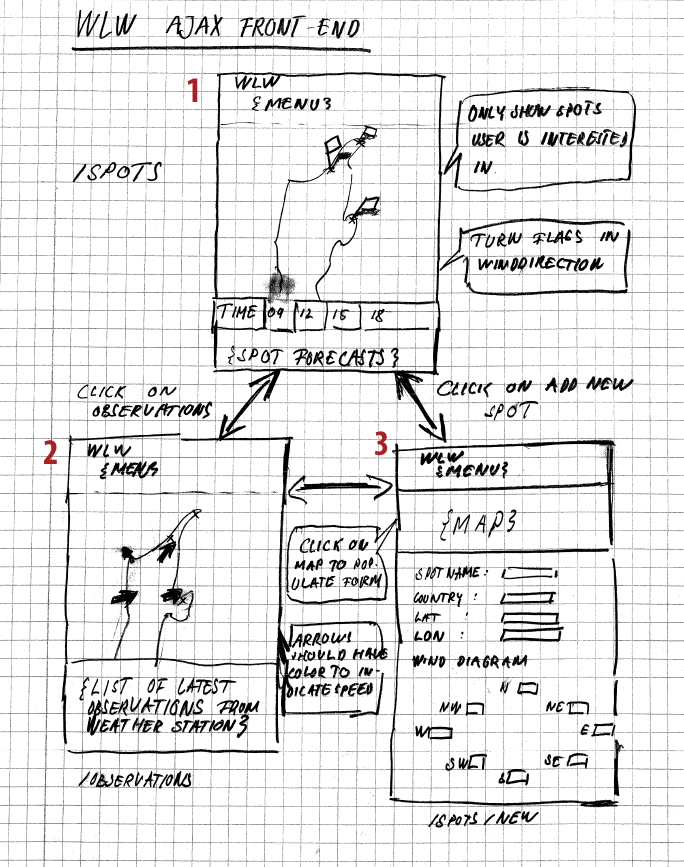
\includegraphics[width=\textwidth]{./Figures/ajax_ui}
  \caption{Paper prototype of main user interface} 
  \label{fig:ajax_ui}
\end{figure}

\section{Finding the location of the client}
A pivotal requirement for the weather service is delivering location-aware
geographic information. This demands that the location of the client is known.
Ideally, the user client tracks the user's location by any available means, e.g.,
IP-address, GPS, or GSM localization, sends the geographic information to the
server that responds with a resource representation relevant for the location. W3C is working
on the Geolocation API Specification that embrace the requirement
\citep{w3:geo_api}. The specification is novel but browsers vendors have begun
supporting it in their beta versions, e.g.,
Opera\footnote{\url{http://my.opera.com/core/blog/geolocation-enabled-build}} and
Mozilla\footnote{\url{https://developer.mozilla.org/En/Using_geolocation}}.

The API is obviously the future, however, the API is not yet supported to an
extent where we would consider using it. At the moment a more viable approach is
using the Google Gears Geolocation
API\footnote{\url{http://code.google.com/apis/gears/mobile.html}}, which among
others the W3C Geolocation API specification builds upon. Google Gears also
support mobile devices, however, only a handful.

JavaScript that use Google Gears triggers a popup in browsers. The popup ask
users to grant permission to the Web application in order to store information on
their computer. The popup is intimidating for users and a sole reason for
another solution.

\url{ipinfodb.com} is a free geolocation service. The service converts from IP
address -- uri-encoded in a GET request -- to a geographical position returned in
either XML or JSON(P). An example: a request such as
\begin{verbatim}
http://ipinfodb.com/ip_query.php?output=json&callback=foo
\end{verbatim}
returns a JSON object wrapped in the \verb|foo| function indicating the
approximate location of the callers computer. Since the returned format is valid
JavaScript requests are directly loaded from the source into client, it just have
to be dynamically inserted into the \verb|<script>| tag. Luckily, jQuery
abstracts that away in the \verb|getJSON| function.

Listing~\ref{lst:iploc} shows how the We Love Wind client uses
\verb|ipinfodb|. The client avoids calling \verb|ipinfodb| repeatedly by storing
the result of the first request as a cookie that is valid for one day.\footnote{A
thorough introduction to cookies in JavaScript is available at
\url{http://www.quirksmode.org/js/cookies.html}} \verb|getLocation| is the entry
function; when a location cookie is not present the client fetches its own
location from \verb|ipinfodb| using \verb|geoIP| and JSON(P).

\begin{lstlisting}[caption=Tracking client location with ipinfodb and JSONP, label=lst:iploc]
// get the lat/lon of this user ip address
function geoIP(callback){
    jQuery.getJSON("http://ipinfodb.com/ip_query.php?output=json&callback=?", function(data){
        var lat = data.Latitude;
        var lon = data.Longitude;
        callback({
            'lat': lat,
            'lon': lon
        });
    });
}

// get the lat/lng of the client
// if location cookie is set get this
function getLocation(callback){
    var location = readCookie('location');
    if (location) {
        var latlng = location.split(',');
        callback({
            'lat': latlng[0],
            'lon': latlng[1]
        });
    }
    else {
        geoIP(function(obj){
            createCookie('location', obj.lat + ',' + obj.lon, 1); // 1 day
            callback(obj);
        });
    }
}
// set location cookie
function setLocation(point) {
	createCookie('location', point.lat + ',' + point.lon, 1);
}  
\end{lstlisting}

\section{Reducing the data set}
The size of the application's data set that the client downloads will eventually
reach a significant size. A size that will hurt the client in terms of increased
latency and poor performance. The geohash grid is a natural means to reduce the
data set. We decrease the amount of data to download by reducing data to
geographical points that are in the neighbors geohash
area. Figure~\ref{fig:geohash_demo} shows the concept; only points within the
boxes are downloaded.


\begin{figure}[htbp]
  \centering
  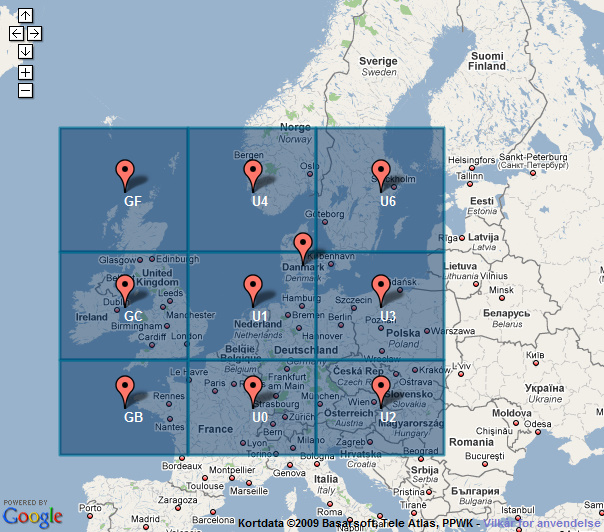
\includegraphics[width=\textwidth]{./Figures/geohash_demo}
  \caption{Geohash grid}
  \label{fig:geohash_demo}
\end{figure}  


The Web Service already supports geohash queries. However, the approach demands
that geohash encoding and grid neighbor finding is also in place at the
client. \citep{geohash:neighbors} is an open source geohash and grid neighbor
finding implementation. We have made the implementation compatible with most
browsers (removing non-standard ECMAscript) and added logic to handle case three
of navigating to neighbors (see Section~\ref{sec:lost}) and included it in the
client.

With geohash in place the client needs a transparent way of handling 1)
downloading points of different types: spots, weather stations, and forecasts
points, and 2) panning of the map which should trigger download of data from
untouched grid boxes. 

The two requirements is accomplished with the publish-subscribe pattern
\citep{Gamma:1995}. A geohash publisher is connected to the map subscribing to
map movement finished events. Upon such events the geohash publisher encodes
the geohash value of the new center, calculates all the neighbors, and publishes
all new geohashes to the subscribers.

We encourage the reader to access
\url{http://www.welovewind.com/examples/geohash/index.html} for a demonstration
of the concept.

\section{Seamless points loading}
With the geohash publisher in place we turn to the problem of seamlessly
downloading points in the published geohash grid cells and displaying the
downloaded points on the map. 

\begin{figure}[htbp]
  \centering
  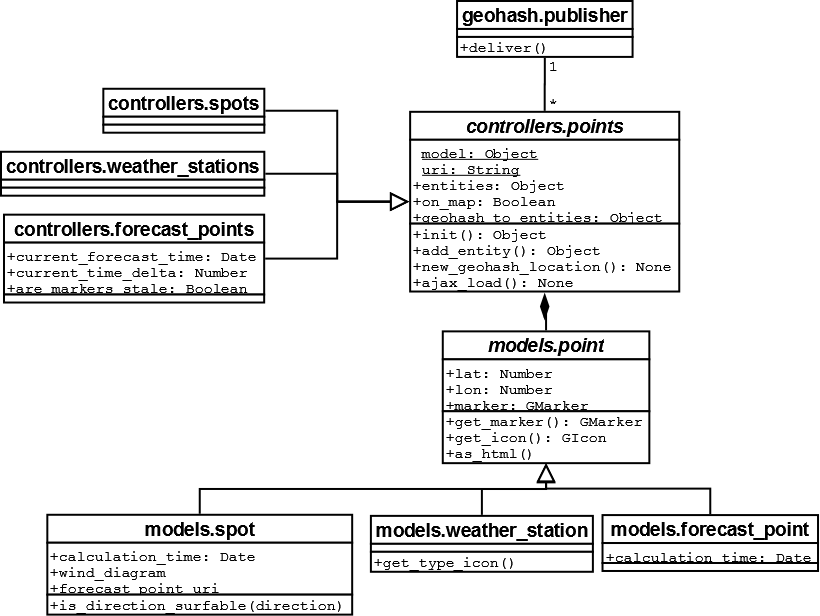
\includegraphics[width=\textwidth]{./Figures/js_model}
  \caption{Client architecture view (UML static structure diagram)}
  \label{fig:js_arch}
\end{figure}

All active geographical points are handled by a points controller, shown in
Figure~\ref{fig:js_arch}. The points controller contains logic to retrieve points
from the server given a geohash. In addition, other objects (not included in the
figure) can subscribe to the points controller, in which case the controller
delivers downloaded points to them. The application currently has three
different types of points: spots, weather stations, and forecast points that all
inherit from the points controller. The ``subclass'' defines the URI of the
concrete Web Service resource, and defines the model for the concrete objects in
the JSON items list (present in all JSON list resources). The model is used to
augment the loaded JSON objects with logic, e.g, to display themselves on a map,
and determine the surfable direction of a spot.

An example of a subscriber of the points controllers is the map controller. The
map controller's responsibility is showing / removing categories of markers on
the map. Figure~\ref{fig:points_loading} shows the runtime architecture of points
loading, and their display on the map. First, all the publish-subscribe
relationships are setup. In addition, a map movement finished subscriber is setup
in the geohash publisher; the subscriber is the source that starts the following process:
\begin{enumerate}
  \item Upon a map movement finished event the geohash for the center of the map
is calculated.
  \item The neighbors are found and subscribers (the points controllers) are
delivered all new touched geohash grid cells.
  \item The points controllers then contact the server for points in the geohash
  cells.
  \item Upon return the points are de-serialized and augmented with logic. The augmented points are delivered
  to the subscribers, in this case, the map controller. 
  \item The map controller adds the points to the map.
\end{enumerate}

The architecture decouples objects and separates concerns. An advantage is that
any other controller interested in points can just add itself as a subscriber to
the different type of points it is interested in. 

\begin{figure}[htbp]
  \centering
  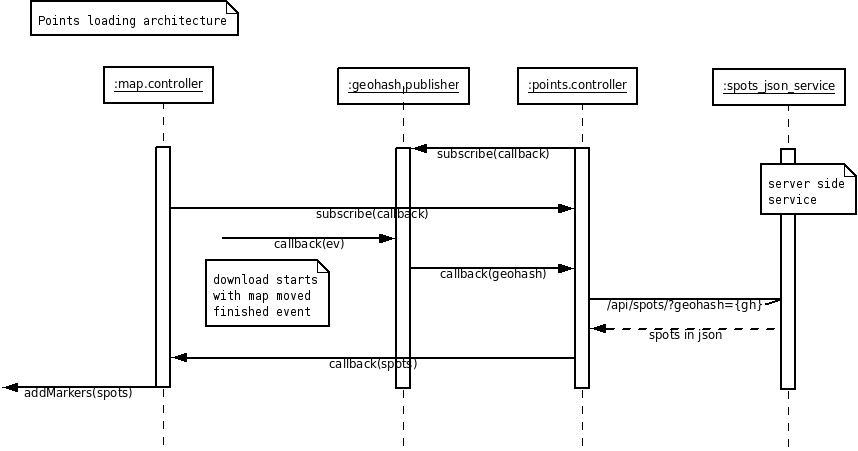
\includegraphics[width=15cm]{./Figures/arch_ajax_points}
  \caption{Points loading architecture view (UML sequence diagram)}
  \label{fig:points_loading}
\end{figure}

\section{Coordination between Ajax calls}
A requirement for the application is visualizing relevant forecasts coupled to
the surfability of spots. We have come up with a graph to visualize the current
and future surfability of spots, shown in Figure~\ref{fig:graph}.\footnote{The
graph is created with the open source jQuery-based graph tool flot:\\
\url{http://code.google.com/p/flot/}} An upward bar in the figure indicates that
the wind is in the correct direction (input by the users), and downward direction
means the wind is in the wrong direction. The colors correspond to the color map
in Figure~\vref{fig:frv}, except that when the wind direction is unsuitable the
color is black.

\begin{figure}[htbp]
  \centering
  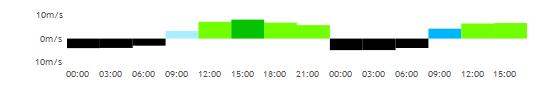
\includegraphics[width=\textwidth]{./Figures/graph}
  \caption{Surfability graph}
  \label{fig:graph}
\end{figure}

The graph demands the presence of both the spot and its corresponding forecast
point. With Ajax the ordering of returned calls is arbitrary. Thus, the client
should somehow coordinate the dependent requests and first when both points are
loaded create the graph.

Every points controller maintain a map from geohash to concrete point
entities. Whenever points from a new geohash are loaded they are inserted into
the map. When controllers subscribe to a points controller they specify a
list of dependencies in the form of references to other points controllers. When
points controllers publish updates to its subscribers the dependencies are
first checked and only if all have downloaded points from the geohash the
callback is triggered. Listing~\ref{lst:points.publish} shows the \verb|publish|
function in the common points controller that handles dependencies.

\begin{lstlisting}[caption=Dependency aware publish function,label=lst:points.publish]
// publish new points loaded
// Args:
//    geohash_prefix: geohash prefix of loaded models
points.publish = function(geohash, the_points){
  // publish points to subscribers
  subscribers_loop: for (var i = 0; i < points.subscribers.length; i++) {
    // check if dependencies are loaded
    for (var j = 0; j < points.subscribers[i].dependencies.length; j++) {
      var controller = points.subscribers[i].dependencies[j];
        
      // if other not loaded continue with next subscriber
      if (!controller.geohash_to_entities[geohash]) {
        continue subscribers_loop;
      }
    }
    // callback(points)
    points.subscribers[i].callback({
      'geohash': geohash,
      'points': the_points
    });
  }
}
\end{lstlisting}

\section{Drawing a circle with Google Maps}
The user interface creates surfability graphs for spots within a certain radius
of the user's location. The user interface needs some component
that indicates this radius to the user and let them adjust it. We apply a
circle as the means to indicate to users the radius of graph creation.

The Google Maps API provides no built-in functionality to draw circles on a
sphere. The API provides a \verb|GPolygon| that can be used to create arbitrary
geometry. There are examples of how to create a circle out of
polygons\footnote{Google Maps circle example:
\url{http://maps.forum.nu/gm_sensitive_circle2.html}}, however, none derive nor
explain the theory of the circle creation. In \citep{haver:veness} many
geographical information systems formulas for JavaScript are presented, however,
it contains no explanation. In the following, we derive the formula behind circle
creation.

\begin{figure}[htbp]
  \centering
  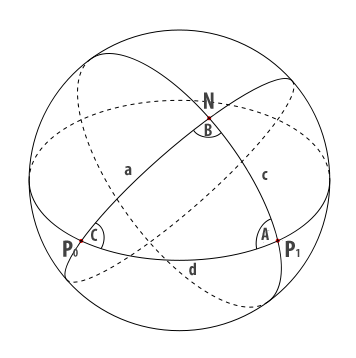
\includegraphics[width=8cm]{./Figures/circle_point}
  \caption{Spherical triangle on sphere} 
  \label{fig:sphere_distance}
\end{figure}

The first requirement is given a point, that will be the center of the circle,
find another point in a certain distance, and bearing from the center point. The
law of cosines, Theorem~\ref{thm:law_of_cosines}, can be used to find points in a
certain distance and bearing from another point. First we find the latitude of
that point.

\subsection*{Latitude}
Given the spherical triangle in Figure~\ref{fig:sphere_distance}, then 
\begin{equation}
  cos(c) = cos(a)cos(d) + sin(a)sin(d)cos(C) \tag{law of cosines}
\end{equation}
Let N be the North Pole, then the distances $a$ and $c$ is given by the
latitudes $P_0$ and $P_1$ respectively. Therefore,
\begin{equation}
  cos(\frac{\pi}{2} - P_{1_{lat}}) = cos(\frac{\pi}{2} - P_{0_{lat}})cos(d) + sin(\frac{\pi}{2} - P_{0_{lat}})sin(d)cos(C) \notag
\end{equation}
Since $cos(\frac{\pi}{2} - \phi) = sin(\phi)$,
\begin{equation}
  sin(P_{1_{lat}}) = cos(P_{0_{lat}})cos(d) + cos(P_{0_{lat}})sin(d)cos(C) \notag
\end{equation}
That is, given a point $P_0$, another point $P_1$ in bearing $C$ and distance $d$
from $P_0$, the latitude of the point $P_1$ is given by
\begin{equation}
  P_{1_{lat}} = asin(cos(P_{0_{lat}})cos(d) + cos(P_{0_{lat}})sin(d)cos(C)) \notag
\end{equation}

% http://en.wikipedia.org/wiki/Spherical_trigonometry
\subsection*{Longitude}
From the last subsection the latitude of the new point is now known. Given that
the angle $B$ on the figure is known, the longitude of the new point,
$P_{1_{lon}}$ is given by
\begin{equation} 
P_{1_{lon}} = P_{0_{lon}} + B \label{eq:longitude_circle}
\end{equation}
We now derive a formula for the angle $B$. Given the spherical triangle in
Figure~\ref{fig:sphere_distance}, then
\begin{equation}
cos(d) = cos(a)cos(c) + sin(a)sin(c)cos(B) \notag
\end{equation}
Let N be the North Pole, then the distances $a$ and $c$ is given by the latitudes
of $P_1$ and $P_0$ respectively. Since $cos(\frac{\pi}{2} - \phi) = sin(\phi)$,
\begin{equation}
cos(d) = sin(P_{0_{lat}})sin(P_{1_{lat}}) + cos(P_{0_{lat}})cos(P_{1_{lat}})cos(B) \notag
\end{equation}
Isolating $B$,
\begin{equation}
cos(B) = \frac{cos(d) - sin(P_{0_{lat}})sin(P_{1_{lat}})}{ cos(P_{0_{lat}})cos(P_{1_{lat}})} \notag
\end{equation}
\begin{equation}
B = acos(\frac{cos(d) - sin(P_{0_{lat}})sin(P_{1_{lat}})}{ cos(P_{0_{lat}})cos(P_{1_{lat}})}) \notag
\end{equation}
The value for $B$ can now be inserted in (\ref{eq:longitude_circle}). Since
$acos$ returns the value in $[0;\pi]$ we have to handle the case when the bearing
is above $\pi$. In that case,
\begin{equation} 
P_{1_{lon}} = P_{0_{lon}} - B
\end{equation}
%
The very observant reader might have noticed something peculiar: the formula
derived does not match with the formulas used in the referred examples and
\citep{haver:veness}. Deriving the formulas used in those are much more
complicated and since they lack explanation it remains uncertain why they did
it that way.

From a mathematical perspective an interesting point is that the whole
theory, both for the distance formulas and the circle formulas breaks
down when one of the points is the North Pole. In that case the
``triangle'' is a line. In practice, however, it is not a problem
since on Google Maps it is not possible to get a point at 90�
latitude. It returns ca. 89.6�.

\subsection*{JavaScript implementation}
With the formulas in place it is easy to implement the function that finds a new
point in a certain bearing and distance from an originating point,
Listing~\ref{lst:javascript_destination} shows how. The function directly
reflects the formulas; because of small rounding errors $cos(B)$ might be larger
than 1, in that case we set it to one to avoid invalid input to $acos$.

\begin{lstlisting}[label=lst:javascript_destination,caption=Finding a point in a certain bearing and distance with JavaScript]
// Calculate a new point in the given bearing and distance
// from the given point
// Args:
//     point: GLatLng to calculate from
//     bearing: bearing in radians  
//     distance: distance to point
function destination(point, bearing, distance){
    var R = 6367; // earth's mean radius in km
    var d = distance / R; // unit sphere distance
    var P0_lon = point.lngRadians();
    var P0_lat = point.latRadians();
    
    var P1_lat = Math.asin(
        Math.sin(P0_lat) * Math.cos(d) + 
        Math.cos(P0_lat) * Math.sin(d) * Math.cos(bearing)
    );
    
    var cos_B = (Math.cos(d) - Math.sin(P0_lat) * Math.sin(P1_lat)) / 
        (Math.cos(P0_lat) * Math.cos(P1_lat));
    
    // secure against rounding errors.
    if(cos_B >= 1){
      cos_B = 1;
    }
  
    if(bearing > Math.PI) {
      var P1_lon = P0_lon - Math.acos(cos_B);
    }else{
      var P1_lon = P0_lon + Math.acos(cos_B);
    }
    // convert to degrees
    P1_lat = P1_lat * (180 / Math.PI);
    P1_lon = P1_lon * (180 / Math.PI);
    return new GLatLng(P1_lat, P1_lon);
};
\end{lstlisting}
Creating the circle on Google Maps is done by iterating from $[0;2\pi]$ creating
a list of points around the center with \verb|destination| and connecting them in
a \verb|GPolygon|.

\section{Summary}
In this chapter we presented the design of the Ajax client and the main
subtleties in the implementation of the client. The subtleties included 1)
loading points on a proximity basis, 2) loading additional points as users pans a
Google Map, 3) coordination of points loading, and 4) drawing a circle with
Google Maps.


\begin{savequote}[10pc]
\sffamily
``Focus on people -- their lives, their work, their dreams.``
\qauthor{Google}
\end{savequote}

\lstset{language=Python}
\chapter{Interface for mobile devices}\label{chap:mobile}
In a context where the users of the application would rather be out surfing than
sitting home by their computer a mobile interface is essential. The application's
interface for mobile devices lets users access the weather service while on the
go. In this chapter, we describe the design and implementation of such an
interface for mobile devices, available at \url{http://m.welovewind.com/}.

In theory the mobile application could be situated at another domain, requesting
the data from the Web service over the network. However, since it is convenient
and faster to directly access the data models of the application we couple the
mobile interface to the Python data models, already presented.

%http://www.codeproject.com/KB/mobile/DeepCast.aspx
%http://www.skyhookwireless.com/devices/devicesupport.php  

\section{Design}
Most mobile devices have small screens, reduced computing power, reduced input
capabilities, and in general fewer functionalities than a standard computer. The
limitations mean that most mobile browsers are unable to render the standard
pages of the application since they rely on JavaScript; in addition, if they
could, the network latency and cost due to the size of the pages would be
significant. Therefore, the mobile version of the weather service calls for a
complete redesign and restructuring of the content, however, the overall
requirement is still the same: to present weather information that assist
practitioners of wind sports.

Figure~\ref{fig:mob_prototype} shows an early manifestation of the mobile user
interface: a user interface paper prototype. The prototype handles
Scenario~\ref{scenario:one} and Scenario~\ref{scenario:two}. Page number 1 on
the figure, is a form where the user must input his location by name. Since the
user most likely need information about the same location on the next visit, the
user's last entered location is automatically set in the form.

Users arrive at page 1 also when accessing the main URI with a mobile
device. Users therefore are relieved of 1) guessing the URI of the mobile page,
or if that is unsuccessful 2) using a search engine to find it.

The main content page of the mobile interface incorporates a concise version of
interesting location-based information, in a wind sports context. The page shows
spots in the proximity, weather observations from weather stations in the
proximity, and the weather forecast from the nearest forecast point. 

Page number 2 gives an all information about the current weather conditions. Page
4 is a map that shows spots and weather stations in the proximity of the
user. The map is important when the user needs to find the way to a new
spot. Page 3 and 5 are pages that show additional information about spots and
weather stations respectively.

\begin{figure}[htbp]
  \centering
  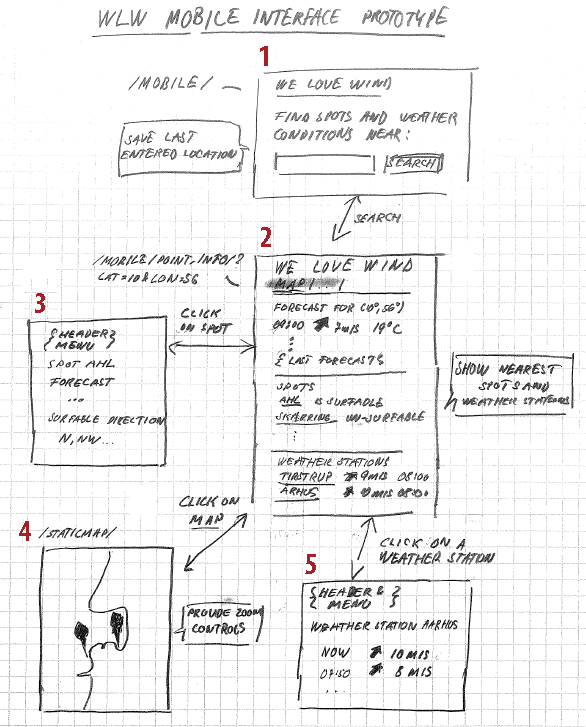
\includegraphics[width=12cm]{./Figures/mobile_prototype}
  \caption{Paper prototype of mobile interface}
  \label{fig:mob_prototype}
\end{figure}

The design discussed in the previous section adds four resources to the
application; the resources are shown in Table~\ref{tab:mobile_resources}. 

\begin{table}[htbp]
\centering \setlength\extrarowheight{3pt}
\begin{tabularx}{\textwidth}{l X X}
\toprule
Resource URI    & Query Parameters & Action\\\midrule
\verb|/mobile/|          & &\verb|GET| search page\\
\verb|/mobile/geo/|      & \verb|location| name &\verb|GET| geocoded location name\\
\verb|/mobile/info/|     & \verb|lat| latitude, 
                           \verb|lon| longitude, 
                           \verb|address| address & \verb|GET| all information for point\\
\verb|/mobile/map/|      & \verb|clat| latitude of center, 
                           \verb|clon| longitude of center,
                           \verb|zoom| zoom level of map,
                           \verb|spots| list of spot keys,
                           \verb|wss| list of weather station keys & \verb|GET| map with spots and weather stations centered around the given point\\
\bottomrule
\end{tabularx}
\caption{Resource view of mobile resources}\label{tab:mobile_resources}
\end{table}

\section{Sorting out the resource requirements}
In the last section we investigated the requirements and pointed out the
additional resources the requirements of the mobile client added to the Web
Service.  Some of the resource content requires somewhat non-trivial processing,
e.g., detecting a mobile client, displaying static maps apt for mobiles without
JavaScript, and converting times to a user relevant timezone. This section
reviews our solutions.

\subsection{Location-based mobile services}
Making a single location-based solution accessible for all browser clients
including mobile ones is impossible at the moment. 

More low level solutions like \citep{sun:lbs} exists, however, they rely on
technologies that are not ubiquitous either. We end up with a solution that rely
on mobile browsers rendering simple HTML pages with no JavaScript. More advanced
solutions could be developed, but the requirement is a widely accessible
solution. In addition, some of the advanced phones, e.g., iphone, are capable of
presenting the main page, see Figure~\ref{fig:iphone}. That is the mobile service
is a lowest common denominator solution.

\begin{figure}[htbp]
  \centering
  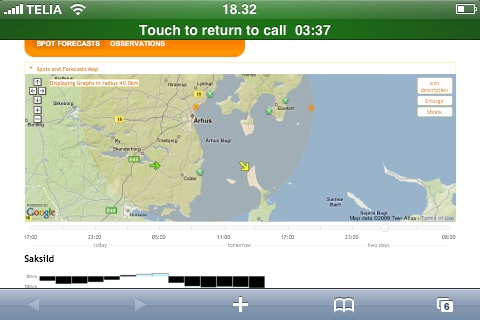
\includegraphics[width=10cm]{./Figures/iphone}
  \caption{Main page on iphone}
  \label{fig:iphone}
\end{figure}

\subsection{Content Negotiation}
Content negotiation is a term defined in \citep[sec.12]{w3:HTTP} which is a
mechanism to serve a representation of a resource based on the capabilities of
the client. In case of the application, users accessing the site with a mobile
should be served representations apt for mobile devices. All browsers populate
the user agent field in HTTP headers; this can be used to decide if the user is
accessing the site from a mobile device.

\begin{lstlisting}[caption=Mobile user agent detection, label=lst:mob_detection]
# special handling of theese
import logging
user_agents = ['ipod', 'android', 'opera mini', (...)]
# mobile user agents trimmed
more_user_agents = ['1207', '3gso', '4thp', '501i', (...)]

def mobile_device(request):
    '''Mobile device detection.
    
    Based on: 
        http://detectmobilebrowsers.mobi/
    Args:
        request: HTTP request
    Returns:
        bool indicating whether the user agent is a mobile device or not.
    '''
    # e.g., User-Agent: Opera/9.60 (J2ME/MIDP; Opera Mini/4.2.13918/422; U; da)
    user_agent = request.META['HTTP_USER_AGENT'].lower()
    logging.info('mobile.mobile_device: user_agent: %s' % user_agent)
    if 'iphone' in user_agent:
        return False
    for ua in user_agents:
        if user_agent.find(ua) != -1:
            return True
    if user_agent[0:4] in more_user_agents:
        return True
    return False
\end{lstlisting}

Listing~\ref{lst:mob_detection} shows the implementation, inspired by a PHP
implementation by \citep{mob:detection}, of user agent detection. The code contains
a list of mobile user agents and detects whether the user agent of the request is
one of them.

When the main page of the application is accessed the content negotiation is
performed. Listing~\ref{lst:cont_negotiation} shows how the root controller take
advantage of the content negotiation.  

HTTP caching is used to bypass the content negotiation on additional accesses to
the page from the same type of user agent.

\begin{lstlisting}[caption=Content negotiating controller,label=lst:cont_negotiation]
from wlw.helpers import mobile

from django import http

def index(request):
    '''Render the index page'''
 
    if mobile.mobile_device(request):
        response = http.HttpResponseRedirect('/mobile/')
    else:
        response = http.HttpResponseRedirect('/observations/')                                      
        response['Vary'] = 'User-Agent' # content varies by user-agent
        response['Cache-Control'] = 'public, max-age=604800' # cache for one week
    return response
\end{lstlisting}

\subsection{Local time}
In the Ajax client, JavaScript converted the UTC times of weather data served from
the Web Service to local times using the timezone of the user's machine. The
mobile interface must work without JavaScript demanding the time conversion to be
done at the server. There are three ways to realize the requirement for serving
time in a sensible timezone format:
\begin{itemize}
  \item let the user input timezone and save it as a cookie;
  \item associate user accounts with timezone information; or
  \item report times in the timezone where it applies.
\end{itemize}
The first and second demands the user to input timezone; whereas, the last
approach totally relieves the user for any input regarding the issue. Picking the
last solution, however, puts forth additional requirements of storing timezone
with all weather data owners: weather stations and forecast points. 

In Chapter~\ref{chap:gae_ws} the Forecast controller and Spot controller
retrieved timezone information from an external Web Service:
\url{http://www.geonames.org/}; it is now evident why: namely to realize option
number three. 

GeoNames is a free database containing extensive geographical
information. GeoNames provide access to its resources through different mainly
RESTful Web Services, and serves representations in XML and JSON formats. The
applied service is the timezone service.

The implementation of code that retrieves a timezone from a point from GeoNames
is shown in Listing~\ref{lst:geonames_tz}. The code uri-encodes the point, fetches
the resource, and handles different failures.

\begin{lstlisting}[caption=Using GeoNames timezone Web Service, label=lst:geonames_tz]
def geonames_timezone(point):
    '''Get timezone information with geonames.org.
    
    Returns:
        json string {'time':..., 'countryName': ..., 'countryCode':..., 'timezoneid': ...}
    '''
    values = {'lat':point.lat, 'lng':point.lon}
    query = http.urlencode(values)
    timezone_uri = 'http://ws.geonames.org/timezoneJSON?%s' % query
    try:
        response = urlfetch.fetch(url=timezone_uri)
        if response.status_code != 200:
            raise WSException('geonames.org not available')
        if 'message' in response.content:
            json = simplejson.decode(response.content)
            raise WSException('ws.geonames.org: %s' % json['status']['message'] )
        return response
    except DownloadError, e:
        raise WSException('geonames.org not available')
\end{lstlisting}

With the timezone in place the times are converted with the logic presented in
Section~\ref{sec:gae_tz}.


\subsection{Geocoding}
Geocoding is applied in order to map from the user input location names to a
latitude and longitude location. There are several geocoding services:
Yahoo\footnote{http://local.yahooapis.com/MapsService/V1/geocode},
GeoNames\footnote{http://www.geonames.org/export/geonames-search.html}, and
\citep{google:geo}.

GeoNames is free, however, the author has experienced low availability of the Web
service. Yahoo, restricts the number of geocoding requests to 5000 pr. day pr. IP
address. Google restricts their service to uses that includes displaying markers
on a Google map. The Google \gls{gls:geocoding} service is chosen, since the mobile
interface presents markers on a Google map. 

Listing~\ref{lst:google_geo} shows how the service is put to use from GAE. The
code takes the following sequence of steps:
\begin{itemize}
  \item Builds an URI to the Google Web service to query. 
  \item Handles different failures, and throw a custom exception if so.
  \item Decodes and inserts the JSON response into a data structure.
  \item Uses memcache to bypass the \gls{gls:geocoding} service, and speed up
additional requests for the same location.
\end{itemize}

\begin{lstlisting}[caption=Google geocoding in Python, label=lst:google_geo]
def google_geocode(location):
    '''Geocode by location name.
    Args:
        location: name of location.
    Returns:
        location info as dictionary {'lat':..., 'lon':...,'address':...}
    '''
    data = memcache.get('/geo/location/%s' % location)
    if data is not None:
        return data 
    else:
        values = {'key': settings.GOOGLE_APP_ID,'q': location, 'output':'json', 'oe':'utf8', 'sensor': 'false'}
        query = http.urlencode(values)
        geocoding_uri = 'http://maps.google.com/maps/geo?%s' % query
        response = urlfetch.fetch(url=geocoding_uri)
        if response.status_code != 200:
            raise WSException('Error finding location')
        json = simplejson.loads(response.content)
        status_code = json['Status']['code']
        if status_code >= 500:
            raise WSException('Could not find location')
        placemark = json['Placemark'][0]
        lat = float(placemark['Point']['coordinates'][1])
        lon = float(placemark['Point']['coordinates'][0])
        address = placemark['address']

        data = {'lat':lat,'lon':lon, 'address':address} 
        if lat and lon and address:
            memcache.add('/geo/location/%s' % location, data)
        return data
\end{lstlisting}

\subsection{Displaying static Google maps}
Google Static
Maps\footnote{\url{http://code.google.com/apis/maps/documentation/staticmaps/}} is a
Web Service that takes an HTTP request generates a static map images and responds
with the image. The service is useful in a context where JavaScript is
unavailable such as our mobile service.

It is easy to put the Static Maps Web Service to use, e.g., retrieving a map of
Denmark is done by issuing a request to the URI:
\begin{verbatim}
http://maps.google.com/staticmap?center=56,10&zoom=6&size=512x512&
        maptype=mobile&sensor=false  
\end{verbatim}
Since the representation format is an image format the URI can be placed in a
usual \verb|img| tag in HTML documents.
\begin{verbatim}
<img src="http://maps.google.com/staticmap?center=56,10&
zoom=6&size=512x512&maptype=mobile&sensor=false />  
\end{verbatim}
Markers on the static map are specified by defining a list of marker descriptors
and setting them as the value of the URI parameter \verb|markers|. A URI
parameter such as
\begin{verbatim}
...&markers=56,10,blue1|57,10,blue2&...
\end{verbatim}
indicates a resource with two marker descriptors that each contains a blue marker
at a specified point. It is possible to suffix marker colors with a single
character that is shown inside the marker, in this case \verb|1| and \verb|2|,

The application dynamically creates the relevant URIs to a static map resource,
and inserts them into the mobile map page. Listing~\ref{lst:gsmaps_creator} shows two
functions: \verb|create_static_markers| and \verb|gsmap_uri|. The former method
takes any list of points and converts them to an appropriate string with a list
of marker descriptors. The latter sets relevant parameters, uri-encodes them, and
returns the URI to the static map resource.

\begin{lstlisting}[caption=Google Static Maps URI creator,label=lst:gsmaps_creator]
def gsmap_uri(center, markers, zoom=8):
    '''Get the URI of the Static Google Map.
    
    Args:
        zoom: the zoom level.
        markers: string with a list of marker descriptors to put on the map.
    Returns:
        the URI of the map resource.
    '''
    values = {
        'size': '200x200',
         # precision of points is 6 decimals
        'center': '%s,%s' % (round(center.lat,6), round(center.lon,6)),
        'maptype':'mobile',
        'markers': markers,
        'key':settings.GOOGLE_APP_ID,
        'sensor':'false',
        'format':'jpg',
        'zoom':zoom
        }
    query = urlencode(values)
    return 'http://maps.google.com/staticmap?%s' % (query)

characters = '123456789abcdefghijklmnopqrstuvwxyz'
   
def create_static_markers(places, color = ''):
    '''Create markers for Google Static Maps API.
    
    Args:
        places: list of points
        color: ('black'| 'brown'| 'green'| 'purple'| (...)
    Returns:
        a string of markers like "10,50,blue1|10,55,blue2".
    '''
    markers = []
    for index, p in enumerate(places):
        marker = '%s,%s,%s' % (round(p.point.lat, 6), round(p.point.lon, 6), color)
        if index < len(characters):
            marker += '%s' % (characters[index])
        markers.append(marker) 
    return '|'.join(markers)
\end{lstlisting}


\section{Implementation}
The implementation is a typical server side Web application: on requests the
server assembles a HTML page and sends it to the client. 

\subsection{Controllers}
The requirements for the mobile application yield four new resources. We skip
presenting the regular expressions, mapping URIs to controller methods, and jump
directly to the implementation of the controllers.

\subsubsection{Search and Geo controller}
The Geo controller handles \gls{gls:geocoding} of the location names
input by the user on the search page. After a successful geocoding the controller
saves the result in a cookie, which enable the last location to automatically be
presented on additional visits to the search page. We skip the code for the
search controller since it only checks for the presence of the cookie, and
renders the search form. 

With the geocoder in place the controller is left off handling exceptions and
setting the cookie. The geocoded address is converted to a byte string before
setting it as a cookie since they can only contain ascii data. After a successful
geocode the controller returns a redirect to the info resource.

\begin{lstlisting}[caption=Geo controller, label=lst:geo_controller]
  def geo(request):
    location = request.GET.get('location', None)
    if location is None:
        http.HttpResponseBadRequest('location must be set')
    try:
        geo = geoinfo.google_geocode(location)
        query = urlencode(geo)
        r = http.HttpResponseRedirect('/mobile/info/?%s' % (query))
        # 2592000 sec. = 1 month
        r.set_cookie('latest_address', smart_str(geo['address']), max_age=2592000)
        return r
    except WSException, e:
        return http.HttpResponse(e)
\end{lstlisting}

\subsection{Map Controller}
Static maps are presented by the map controller. The resource is a typical
algorithmic resource where the uri-parameters can be seen as input into an
algorithm that creates a map. 

The map controller takes as input the latitude and longitude of the center of the
map, and a list of spot and weather station keys, representing points to put on
the map. Point entities are retrieved from the datastore by directly giving them
as a list to the datastore method \verb|get_by_key_name|.

The controller rely on the functions in the \verb|gstaticmaps| module to create
the URI for the static map resource on Google. The controller maintains many
uri-parameters to handle the \textit{\gls{gls:appstate}}, and keeping the server
stateless. An example is the \verb|zoomed| query dictionary that contains a
complete copy of the uri-parameters only deviating on the value of \verb|zoom|.

\begin{lstlisting}
def map(request):
    '''The map page
    
    Args GET:
        clat: center latitude of map
        clon: center longitude of map
        spots: spotkey1;spotkey2;...
        wss: wskey1;wskey2;...
        zoom: the zoom level of the map
    '''
    center_lat = request.GET['clat']
    center_lon = request.GET['clon']
    zoom = int(request.GET.get('zoom', 8))        
    spot_keys = request.GET.get('spots', None)
    wss_keys = request.GET.get('wss', None)
        
    spots, wss = [], []
    if spot_keys:
        spots = Spot.get_by_key_name(spot_keys.split(';'))
    if wss_keys:
        wss = WeatherStation.get_by_key_name(wss_keys.split(';'))

    query_dict = request.GET.copy()
    # zoom in
    query_dict['zoom'] = zoom + 2
    zoomed = query_dict.urlencode()
    # zoom out
    query_dict['zoom'] = zoom - 2 
    zoomed_out = query_dict.urlencode()
    
    spot_markers = gstaticmaps.create_static_markers(spots, 'blue')
    wss_markers = gstaticmaps.create_static_markers(wss, 'green')
    markers = '|'.join([spot_markers, wss_markers])
    
    static_map_uri = gstaticmaps.gsmap_uri(
        db.GeoPt(lat=center_lat, lon=center_lon), markers, zoom)
    
    address = request.GET.get('address')
    
    values = {
        'lat': request.GET.get('lat'),
        'lon': request.GET.get('lon'),
        'address': address}
    
    qs = urlencode(values)
    
    return shortcuts.render_to_response(
        'map_mobile.xhtml',
        {'spots':spots, 'wss':wss, 'static_map_uri':static_map_uri, 'qs': qs,
            'qs_zoomed': zoomed, 'qs_zoomed_out':zoomed_out}        
    )
\end{lstlisting}

\subsection{Info controller}
The info controller provides access to the main mobile content page: page 2 in
the prototype. From a given geographic point the controller retrieves all weather
stations and spots within a 50 km radius, by using the \verb|get_near_point|
method presented in Section~\ref{sec:models}; the method sorts the points by
distance raising the relevance of the first presented points, of each category,
in the user interface. The length of the geohash prefix, input to
\verb|get_by_distance| was chosen on a pure pragmatic basis using the geohash
demonstrator.\footnote{\url{http://www.welovewind.com/examples/geohash/index.html}}

\begin{lstlisting}
def info(request):
    '''Info about a point.
    
    Retrieve spots, weather stations in the proximity, and the forecasts for the point.
    
    Args GET:
        lat: latitude of point
        lon: longitude of point
        address: address of point
    '''
    lat = float(request.GET.get('lat'))
    lon = float(request.GET.get('lon'))
    if lat is None or lon is None:
        http.HttpResponseBadRequest('lat/lon must be set')
    address = request.GET.get('address', '(%s,%s)' % (lat, lon))
    
    center = db.GeoPt(lat=lat, lon=lon)
    
    wss = WeatherStation.get_by_point(center, 50, 3)
    spots = Spot.get_by_point(center, 50, 3)
    forecast_point = ForecastPoint.get_or_init_by_point(center)
    
    spot_keys = [s.key().name() for s in spots]
    wss_keys = [w.key().name() for w in wss]
    
    # the 'list' is just a key string separated by commas in the uri.
    map_values = {
        'clat': lat,
        'clon': lon,
        'spots': ';'.join(spot_keys),
        'wss': ';'.join(wss_keys),
    }
    
    map_uri = '/mobile/map/?%s' % urlencode(map_values)
    
    return shortcuts.render_to_response(
        'info_mobile.xhtml',
        {
            'map_uri':map_uri,
            'spots':spots,
            'wss':wss,
            'fp':forecast_point,
            'qs': request.GET.urlencode(),
            'address': address
        })
\end{lstlisting}


\subsection{Views}
% http://www.w3.org/TR/mobile-bp/
All the views of the mobile interface are valid XHTML Basic 1.1: the W3C
recommendation for content the format for mobile interfaces
\citep{w3c:mobile}. We skip presenting the views of the mobile application. The
interested reader can refer to Appendix~\ref{app:mobile} for the views.

\section{Summary}
In this chapter, we extended the application with a mobile interface, to support
scenarios where the user is on the go. The mobile interface had a significant
impact on the application in terms of complexity. The added complexity stems from
1) a requirement for the mobile application being widely accessible, and 2) the
limit of many mobile browsers. The application could not rely on JavaScript, and
therefore functionality already developed in JavaScript, such as timezone
conversion and display of maps, was implemented on the server side also.


%% I can't change the direction of the wind, but I can adjust my sails to always reach my destination. 
%% Jimmy Dean 

% Chapter Conclusion
\part{Conclusion \& Perspectives}

%% \begin{savequote}[10pc]
%%  \sffamily
%% ``I can't change the direction of the wind, but I can adjust my sails to always reach my destination.''
%% \qauthor{James Dean (1931 -- 1955)}
%% \end{savequote}

%\chapter{Conclusion \& Perspectives} % Write in your own chapter title
\label{Conclusion}
Through three parts in this dissertation, The Foundations, The Web Services, and
The Clients, we have reached the destination, a ``Web-Based Weather Service for
Wind Sports''. The integration of these three parts is a mashup that assists the
practitioners of wind sports.

Our dissertation gives an insight into the course we took to 1) extract data from
external resources (independent of format) and, to 2) create a geographical
information system mashup based on that data. The insight includes:
\begin{itemize}
  \item The theoretical foundations for creating mashups
(Chapter~\ref{chap:web}). The foundations included a presentation of the
architectural style REST, the architecture ROA upon which we based our Web
Services, and an infrastructure to run the mashups: the GAE.
  \item Practices for designing the resources in a Web Services
(Chapter~\ref{chap:resources}) and afterwards practices for implementation of
mashups; in our application, manifested in two Web Services: the We Love Wind Web
Service (Chapter~\ref{chap:gae_ws}) and the DAIMI Forecast Web Service
(Chapter~\ref{chap:ws_daimi}). 
  \item At last the insight includes the theoretical foundations for creating an
  Ajax client (Chapter~\ref{chap:ws_clients}) and a mobile client. In addition,
  concrete practices for implementing such clients (Chapter~\ref{chap:client} and
  Chapter~\ref{chap:mobile})
\end{itemize}

Our thesis was only possible because we had access to public weather information
from the US that use the `open access' model \citep{noaa:datareport} for public
sector information. The European model, known as the `cost recovery' model,
restricts access to public data. During the last half year there have been
European initiatives that argue in favor for open access to public
data. \url{digitaliser.dk}, created by the Danish government, is one of the
front-runners, quoting their Web site:
\begin{quote}
Digitalis�r.dk aims to stimulate development and adoption of digital content and
business models by utilising Web 2.0 technologies and public data and digital
resources. 
\end{quote}
\verb|digitaliser.dk| aspires to create common grounds of how to get access to
public sector information. Times are thus changing in favor of mashups.

%% \begin{quotation}
%% \begin{flushright}
%% \textit{Come senators, congressmen\\
%% Please heed the call\\
%% Don't stand in the doorway\\
%% Don't block up the hall\\
%% For he that gets hurt\\
%% Will be he who has stalled\\
%% There's a battle outside\\
%% And it is ragin'.\\
%% It'll soon shake your windows\\
%% And rattle your walls\\
%% For the times they are a-changin'.\\}
%% Bob Dylan (1941--)
%% \end{flushright}
%% \end{quotation}

\part{Appendix \& Glossary}

%% Chapter 1


\begin{savequote}[10pc]
\sffamily
Smoke whirls\\
After the passage of a train.\\
Young foliage.
\qauthor{Shiki Masaoka (1867-1902)}
\end{savequote}
\chapter{\LaTeX{} info} % Write in your own chapter title

\label{Info}

\section{Examples of \LaTeX{} Typeset eBooks}

You can see (and download and read) examples of eBooks typeset by \LaTeX{} in a small library here:\\
\href{http://www.sunilpatel.co.uk/typesetting.html}{\texttt{http://www.sunilpatel.co.uk/typesetting.html}}

The books are available for you to download for free. They were originally plain text files but were quickly and easily converted into beautifully typeset and well presented eBooks through \LaTeX{} for you to enjoy.


\section{Learning \LaTeX{}}

\LaTeX{} is not a WYSIWYG (What You See is What You Get) program, unlike word processors such as Microsoft Word or Corel WordPerfect. Instead, a document written for \LaTeX{} is actually a simple, plain text file that contains \emph{no formatting}. You tell \LaTeX{} how you want the formatting in the finished document by writing in simple commands amongst the text, for example, if I want to use \emph{italic text for emphasis}, I write the `$\backslash$\texttt{emph}\{\}' command and put the text I want in italics in between the curly braces. This means that \LaTeX{} is a ``mark-up'' language, very much like HTML.

\subsection{A (not so short) Introduction to \LaTeX{}}

If you are new to \LaTeX{}, there is a very good eBook -- freely available online as a PDF file -- called, ``The Not So Short Introduction to \LaTeX{}''. The book's title is typically shortened to just ``lshort''. You can download the latest version (as it is occasionally updated) from here:\\
\href{http://www.ctan.org/tex-archive/info/lshort/english/lshort.pdf}{\texttt{http://www.ctan.org/tex-archive/info/lshort/english/lshort.pdf}}

It is also available in several other languages. Find yours from the list on this page:\\
\href{http://www.ctan.org/tex-archive/info/lshort/}{\texttt{http://www.ctan.org/tex-archive/info/lshort/}}

It is recommended to take a little time out to learn how to use \LaTeX{} by creating several, small `test' documents. Making the effort now means you're not stuck learning the system when what you \emph{really} need to be doing is writing your thesis.

\subsection{A Short Math Guide for \LaTeX{}}

If you are writing a technical or mathematical thesis, then you may want to read the document by the AMS (American Mathematical Society) called, ``A Short Math Guide for \LaTeX{}''. It can be found online here:\\
\href{http://www.ams.org/tex/amslatex.html}{\texttt{http://www.ams.org/tex/amslatex.html}}\\
under the ``Additional Documentation'' section towards the bottom of the page.

\subsection{Common \LaTeX{} Math Symbols}
There are a multitude of mathematical symbols available for \LaTeX{} and it would take a great effort to learn the commands for them all. The most common ones you are likely to use are shown on this page:\\
\href{http://www.sunilpatel.co.uk/latexsymbols.html}{\texttt{http://www.sunilpatel.co.uk/latexsymbols.html}}

You can use this page as a reference or crib sheet, the symbols are rendered as large, high quality images so you can quickly find the \LaTeX{} command for the symbol you need.


\section{Thesis Features and Conventions}\label{ThesisConventions}

To get the best out of this template, there are a few conventions that you may want to follow.

One of the most important (and most difficult) things to keep track of in such a long document as a thesis is consistency. Using certain conventions and ways of doing things (such as using the Todo list) makes the job easier. Of course, all of these are optional and you can adopt your own method.

\subsection{References}

The `\texttt{natbib}' package is used to format the bibliography and inserts references such as this one.\citep{Reference3} The options used in the `\texttt{Thesis.tex}' file mean that the references are listed in numerical order as they appear in the text. Multiple references are rearranged in numerical order\citep{Reference2, Reference1} and multiple, sequential references become reformatted to a reference range.\citep{Reference2, Reference1, Reference3} This is done automatically for you. To see how you use references, have a look at the `\texttt{Chapter1.tex}' source file.

References should come \emph{after} the punctuation mark if there is one (such as a comma or full stop). On the other hand, footnotes\footnote{Such as this footnote, here down at the bottom of the page.} come \emph{before} the punctuation mark. You can swap these around but the most important thing is to keep the convention consistent throughout the thesis. Footnotes themselves should be full, descriptive sentences (beginning with a capital letter and ending with a full stop).

To see how \LaTeX{} typesets the bibliography, have a look at the very end of this document (or just click on the reference number links).

\subsection{Figures}

There will hopefully be many figures in your thesis (that should be placed in the `Figures' folder). The way to insert figures into your thesis is to use a code template like this:
\begin{verbatim}
\begin{figure}[htbp]
  \centering
    
\includegraphics{./Figures/Electron.pdf}
    \rule{35em}{0.5pt}
  \caption[An Electron]{An electron (artist's impression).}
  \label{fig:Electron}
\end{figure}
\end{verbatim}
Also look in the source file. Putting this code into the source file produces the picture of the electron that you can see in the figure below.

\begin{figure}[htbp]
	\centering
		
\includegraphics{./Figures/Electron.pdf}
		\rule{35em}{0.5pt}
	\caption[An Electron]{An electron (artist's impression).}
	\label{fig:Electron}
\end{figure}

Sometimes figures don't always appear where you write them in the source. The placement depends on how much space there is on the page for the figure. Sometimes there is not enough room to fit a figure directly where it should go (in relation to the text) and so \LaTeX{} puts it at the top of the next page. Positioning figures is the job of \LaTeX{} and so you should only worry about making them look good!

Figures usually should have labels just in case you need to refer to them (such as in figure \ref{fig:Electron}). The `$\backslash$\texttt{caption}' command contains two parts, the first part, inside the square brackets is the title that will appear in the `List of Figures', and so should be short. The second part in the curly brackets should contain the longer and more descriptive caption text.

The `$\backslash$\texttt{rule}' command is optional and simply puts an aesthetic horizontal line below the image. If you do this for one image, do it for all of them.

The \LaTeX{} Thesis Template is able to use figures that are either in the PDF or JPEG file format. It is recommended that you read this short guide on how to get the best out of figures in \LaTeX{}, available here:\\
\href{http://www.sunilpatel.co.uk/texhelp5.html}{\texttt{http://www.sunilpatel.co.uk/texhelp5.html}}

Though it is geared more towards users of Mac and OS X systems, much of the advice applies to creating and using figures in general. It also explains why the PDF file format is preferred in figures over JPEG.

\subsection{Typesetting mathematics}

If your thesis is going to contain heavy mathematical content, be sure that \LaTeX{} will make it look beautiful, even though it won't be able to solve the equations for you.

The ``Not So Short Introduction to \LaTeX{}'' (available \href{http://www.ctan.org/tex-archive/info/lshort/english/lshort.pdf}{here}) should tell you everything you need to know for most cases of typesetting mathematics. If you need more information, a much more thorough mathematical guide is available from the AMS called, ``A Short Math Guide to \LaTeX{}'' and can be downloaded from:\\
\href{ftp://ftp.ams.org/pub/tex/doc/amsmath/short-math-guide.pdf}{\texttt{ftp://ftp.ams.org/pub/tex/doc/amsmath/short-math-guide.pdf}}

There are many different \LaTeX{} symbols to remember, luckily you can find the most common symbols \href{http://www.sunilpatel.co.uk/latexsymbols.html}{here}. You can use the web page as a quick reference or crib sheet and because the symbols are grouped and rendered as high quality images (each with a downloadable PDF), finding the symbol you need is quick and easy.

You can write an equation, which is automatically given an equation number by \LaTeX{} like this:
\begin{verbatim}
\begin{equation}
E = mc^{2}
  \label{eqn:Einstein}
\end{equation}
\end{verbatim}

This will produce Einstein's famous energy-matter equivalence equation:
\begin{equation}
E = mc^{2}
\label{eqn:Einstein}
\end{equation}

All equations you write (which are not in the middle of paragraph text) are automatically given equation numbers by \LaTeX{}. If you don't want a particular equation numbered, just put the command, `$\backslash$\texttt{nonumber}' immediately after the equation.


\section{Sectioning and Subsectioning}

You should break your thesis up into nice, bite-sized sections and subsections. \LaTeX{} automatically builds a table of Contents by looking at all the `$\backslash$\texttt{chapter}$\{\}$', `$\backslash$\texttt{section}$\{\}$' and `$\backslash$\texttt{subsection}$\{\}$' commands you write in the source.

The table of Contents should only list the sections to three (3) levels. A `$\backslash$\texttt{chapter}$\{\}$' is level one (1). A `$\backslash$\texttt{section}$\{\}$' is level two (2) and so a `$\backslash$\texttt{subsection}$\{\}$' is level three (3). In your thesis it is likely that you will even use a `$\backslash$\texttt{subsubsection}$\{\}$', which is level four (4). Adding all these will create an unnecessarily cluttered table of Contents and so you should use the `$\backslash$\texttt{subsubsection$^{*}\{\}$}' command instead (note the asterisk). The asterisk ($^{*}$) tells \LaTeX{} to omit listing the subsubsection in the Contents, keeping it clean and tidy.


\section{In Closing}

You have reached the end of this mini-guide. You can now rename or overwrite this pdf file and begin writing your own `\texttt{Chapter1.tex}' and the rest of your thesis. The easy work of setting up the structure and framework has been taken care of for you. It's now your job to fill it out! If you use this Thesis template and this mini-guide helps you, please let me know\footnote{Email: \href{mailto:web@sunilpatel.co.uk}{web@sunilpatel.co.uk} all comments and suggestions, questions and errata are welcome.}.

Good luck and have lots of fun!

\begin{flushright}
Sunil Patel: \href{http://www.sunilpatel.co.uk}{www.sunilpatel.co.uk}
\end{flushright}


%% ----------------------------------------------------------------
% Now begin the Appendices, including them as separate files

\addtocontents{toc}{\vspace{2em}} % Add a gap in the Contents, for aesthetics

\appendix % Cue to tell LaTeX that the following 'chapters' are Appendices

%\chapter{Glossary}
%\label{Glossary}

\printglossary
\addcontentsline{toc}{chapter}{Glossary}

% Appendix A

\chapter{Appendix A}
\label{AppendixA}

\section{Rejseplanen.dk screenshots}
When polite search engines, like Googlebot, access pages they first check the
rules in the server's \verb|robots.txt|. In
Figure~\ref{app:fig:rejseplanen_robots} \url{http://www.rejseplanen.dk/robots.txt} is shown;
all crawling is disabled, since \verb|Disallow| is set to \verb|/| for all agents.

\begin{figure}[htbp]
  \centering
  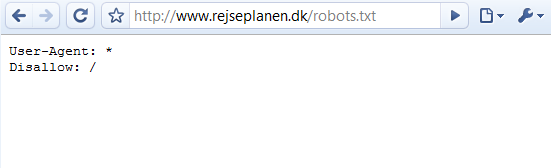
\includegraphics[width=14cm]{./Figures/rejseplanen_robots_110309}
  \rule{\textwidth}{0.005in}
  \caption{{\tt robots.txt} at \url{www.rejseplanen.dk}; [accessed 11-March-2009]}
  \label{app:fig:rejseplanen_robots}
\end{figure}

\begin{lstlisting}[caption=\url{http://www.rejseplanen.dk/},label=lst:rejseplanen.dk]
<!DOCTYPE HTML PUBLIC "-//W3C//DTD HTML 4.01 Frameset//EN">
<html>
  <head>
    <meta http-equiv="Content-Type" content="text/html; charset=ISO-8859-1">
      <title>Rejseplanen</title>
  </head>
  <frameset rows="100%">
    <frame name="rejseplanen" src="/bin/query.exe/mn">
      <noframes>
        <body>
          <a href="/bin/query.exe/mn">Videre</a> til Rejseplanen. L&#230;s mere om
          <a href="http://tog-bus.rejseplanen.dk">rejseplanl&#230;gning med kollektiv trafik</a>.
        </body>
      </noframes>
  </frameset>
</html>
\end{lstlisting}

\section{Cross-site scripting with eval}\label{sec:xss}
Imagine a site where user entered JSON data is de-serialized using the JavaScript
\verb|eval|
function\footnote{\url{https://developer.mozilla.org/en/Core_JavaScript_1.5_Reference/Global_Functions/eval}},
e.g., a site with user entered surf spots. 

Listing~\ref{lst:xss} shows how executing \verb|eval| on the user input --
hardcoded in the site in this example -- executes injected JavaScript. When the
data is evaled, the entered data is executed as if it were JavaScript. This is
used in Listing~\ref{lst:xss} to inject an extra field in the evaled data
structure. The interesting line is this:
\begin{verbatim}
{
	"name": "Ahl", attack: alert('attack'), after:""
}  
\end{verbatim}
Because the value in the \verb|attack| field is not surrounded by "", the command
\verb|alert()| is executed. We notice that this line comes from entering the
following as surf spot name:
\begin{verbatim}
  Ahl'', attack: alert('attack'), after:''
\end{verbatim}

Since it is valid JavaScript syntax, but not JSON syntax the attack is realizable
only if the response is not parsed as JSON. The attack can be tried out in action
by going to \url{http://welovewind.appspot.com/examples/xss.html}.

\begin{lstlisting}[caption=xss.html,label=lst:xss]
<!DOCTYPE html PUBLIC "-//W3C//DTD XHTML 1.0 Strict//EN"
    "http://www.w3.org/TR/xhtml1/DTD/xhtml1-strict.dtd">
<html xmlns="http://www.w3.org/1999/xhtml">
  <head>
    <meta http-equiv="content-type" content="text/html; charset=utf-8"/>
	<title>JSON eval() issues</title>
    
    <script type="text/javascript">
    //<![CDATA[
		function run(id) {
			json = document.getElementById(id).innerHTML;
			res = eval('(' + json + ')');
			return res;
		}
    //]]>
    </script>
  </head>
  <body>
  	<h1>JSON eval() issues</h1>
		<h2>Example</h2>
		<pre id="ex1">
{
	"name": "Ahl", attack: alert('attack'), after:""
}
		</pre>
		<button onclick="run('ex1');">eval it!</button>
  </body>
</html>
\end{lstlisting}	% Appendix Title

%\chapter{Appendix}
\label{app:ws_imp}

\section{Python Implementation of Unique Datastore Property}
Listing~\ref{lst:unique_prop_model} shows the implementation and an example of
the usage of a unique property model. The class is inspired by a method to
retrieve or create an object by its unique
properties\footnote{http://appengine-cookbook.appspot.com/recipe/get-or-insert-entity-by-unique-properties/}.
As the listing shows the unique property model is used by inheriting from it; the
sub model gets an extra classmethod, the \verb|update_or_init_by| method. The
method updates or initializes a model depending on the existence of the unique
properties given as arguments. The model does not guarantee uniqueness in a
concurrent environment.

It is not possible to run the code in a transaction since it does queries, which
are prohibited in transactions; the constraints of transactions are described
in~\cite{Google:transactions}. 

\begin{lstlisting}[label=lst:unique_prop_model,caption=Unique property model]
  
class UniquePropertyModel(db.Model):
    
    @classmethod
    def update_or_init_by(cls, unique_props={}, **kwargs):
        '''Update / initialize an entity.
                
        The entity is not saved in the datastore by this method.
        
        Args:
            unique_props: dict with string / object pairs to apply filters on
            kwds: properties to initialize / update
        Returns:
            the updated / new entity
        '''
        query = db.Query(cls)
        # find the entity by the unique props
        for p in unique_props:
            query.filter("%s =" % p, unique_props[p])
        entity = query.get()
        # if entity exist, update it
        if entity is not None:
            for kw in kwds:
                setattr(entity, kw, kwds[kw])
            return entity
        # init the entity, add props from unique props
        kwds.update(unique_props)
        entity = cls(**kwds)
        return entity

class ExampleModel(UniquePropertyModel):
  name = db.StringProperty()
  email = db.StringProperty()

instance = ExampleModel.update_or_init_by(
  {'email':'test@example.com'}, 
  name='test name')
instance.put()
\end{lstlisting}     
        



% Appendix 

\chapter{Appendix B}
\label{app:mobile}

\section{Implementation of Views for Mobile Devices}
\subsection{Base mobile template}
\lstinputlisting[caption=Base mobile user interface template, label=lst:mob_base_ui]{code/base_mobile.xhtml}

\subsection{Search template}
\lstinputlisting[caption=Search template, label=lst:mob_search]{code/search_mobile.xhtml}

\subsection{Info template}
\lstinputlisting[caption=Info template, label=lst:mob_info]{code/info_mobile.xhtml}

\subsection{Map template}
\lstinputlisting[caption=Map template, label=lst:mob_info]{code/map_mobile.xhtml}





\chapter{Appendix C}
\label{AppendixHaversine}

\section{Comparing Distances Calculated with Haversine and Cosines}

\begin{lstlisting}
def distance_cosines_relation(point1, point2):
    '''Calculates the distance between two points, using the spheric cosines formula.
    '''
    lat1,lon1 = to_radians(point1)
    lat2,lon2 = to_radians(point2)
    a = sin(lat1) * sin(lat2)
    b = cos(lat1) * cos(lat2) * cos(lon2 - lon1)
    c = acos(a + b)
    d = earth_radius * c
    return d  
\end{lstlisting}

\begin{lstlisting}
class Point:
    def __init__(self,lat,lon):
        self.lat = lat
        self.lon = lon

def compare():
    class Point:
        def __init__(self,lat,lon):
            self.lat = lat
            self.lon = lon
    aarhus = Point(56.0,10.0)
    aalborg = Point(57.0, 10.0)
    for i in range(25):
        # distances in m
        cosines_distance = distance_cosines_relation(aarhus, aalborg)
        haversine_distance = distance(aarhus, aalborg)
        difference = cosines_distance - haversine_distance
        print 'P2: (%s,%s)\nHDist: %sm\tCDist:%sm\nDiff:%sm' % \
            (aalborg.lat, aalborg.lon, 
            haversine_distance * 1000, cosines_distance * 1000, difference * 1000)
        print '---------'
        # half distance
        aalborg.lat = aarhus.lat + (aalborg.lat - aarhus.lat) / 2      
\end{lstlisting}

\begin{lstlisting}
P2: (57.0,10.0)
HDist: 111125.113474m	CDist:111125.113474m
Diff:-1.12549969344e-008m
---------
P2: (56.5,10.0)
HDist: 55562.5567372m	CDist:55562.5567371m
Diff:-9.63567003964e-008m
---------
P2: (56.25,10.0)
HDist: 27781.2783686m	CDist:27781.2783686m
Diff:-5.07327513333e-009m
---------
P2: (56.125,10.0)
HDist: 13890.6391843m	CDist:13890.6391843m
Diff:3.37667671602e-008m
---------
P2: (56.0625,10.0)
HDist: 6945.31959215m	CDist:6945.31959159m
Diff:-5.66108049327e-007m
---------
P2: (56.03125,10.0)
HDist: 3472.65979608m	CDist:3472.65979594m
Diff:-1.33233424293e-007m
---------
P2: (56.015625,10.0)
HDist: 1736.32989804m	CDist:1736.32989803m
Diff:-7.03592739626e-009m
---------
P2: (56.0078125,10.0)
HDist: 868.164949019m	CDist:868.164945702m
Diff:-3.31756488947e-006m
---------
P2: (56.00390625,10.0)
HDist: 434.08247451m	CDist:434.082477783m
Diff:3.27316213022e-006m
---------
P2: (56.001953125,10.0)
HDist: 217.041237255m	CDist:217.041228492m
Diff:-8.76289446561e-006m
---------
P2: (56.0009765625,10.0)
HDist: 108.520618627m	CDist:108.520583137m
Diff:-3.54903024608e-005m
---------
P2: (56.0004882813,10.0)
HDist: 54.2603093133m	CDist:54.2602708314m
Diff:-3.84819070012e-005m
---------
P2: (56.0002441406,10.0)
HDist: 27.1301546566m	CDist:27.1301354156m
Diff:-1.9241015066e-005m
---------
P2: (56.0001220703,10.0)
HDist: 13.565077328m	CDist:13.5649018138m
Diff:-0.0001755141407m
---------
P2: (56.0000610352,10.0)
HDist: 6.78253866398m	CDist:6.78211910881m
Diff:-0.00041955517375m
---------
P2: (56.0000305176,10.0)
HDist: 3.39126933199m	CDist:3.39039587702m
Diff:-0.000873454969691m
---------
P2: (56.0000152588,10.0)
HDist: 1.69563466564m	CDist:1.69453406618m
Diff:-0.00110059946489m
---------
P2: (56.0000076294,10.0)
HDist: 0.847817332821m	CDist:0.848593998715m
Diff:0.000776665893623m
---------
P2: (56.0000038147,10.0)
HDist: 0.423908666057m	CDist:0.413553559386m
Diff:-0.0103551066715m
---------
P2: (56.0000019073,10.0)
HDist: 0.211954333029m	CDist:0.212148499679m
Diff:0.000194166650125m
---------
P2: (56.0000009537,10.0)
HDist: 0.105977166514m	CDist:0.0948756933212m
Diff:-0.0111014731931m
---------
P2: (56.0000004768,10.0)
HDist: 0.0529885829037m	CDist:0.0m
Diff:-0.0529885829037m
---------
P2: (56.0000002384,10.0)
HDist: 0.0264942914519m	CDist:0.0m
Diff:-0.0264942914519m
---------
P2: (56.0000001192,10.0)
HDist: 0.0132471457259m	CDist:0.0m
Diff:-0.0132471457259m
---------
P2: (56.0000000596,10.0)
HDist: 0.00662357286296m CDist:0.0m
Diff:-0.00662357286296m
---------
\end{lstlisting}

\addtocontents{toc}{\vspace{2em}}  % Add a gap in the Contents, for aesthetics
\backmatter

%% ----------------------------------------------------------------
\label{Bibliography}
\bibliography{Bibliography}  % The referen (bibliography) information are stored in the file named "Bibliography.bib"

\end{document}
